%% -*- fill-column: 80; comment-column: 50; -*-
\documentclass[a4paper]{report}
% \VignetteIndexEntry{Introduction to Renext}
% \VignetteDepends{Renext}
% \VignetteKeyword{extreme values}
\usepackage{amsmath, amsfonts, amssymb, amsthm}
\usepackage[english]{babel}

\usepackage{url}
\usepackage{fullpage}
\usepackage{boxedminipage}
\usepackage{booktabs}
\usepackage{hyperref}
\usepackage{makeidx}
\usepackage{titlesec}
\usepackage{color}
\usepackage{afterpage}
\usepackage[utf8]{inputenc}

\newcommand\blankpage{%
    \null
    \thispagestyle{empty}%
    \addtocounter{page}{-1}%
    \newpage}

%% bibliography
\if@shortnames
  \usepackage[authoryear,round]{natbib}
\else
  \usepackage[authoryear,round,longnamesfirst]{natbib}
\fi
\bibpunct{(}{)}{;}{a}{}{,}
\bibliographystyle{jss}

\makeindex

%% \parskip=1.5ex plus 1.5ex minus 1.25ex
%% \titleformat{\section}[block]{\normalfont\large\bfseries}{\thesection}{1em}{}
%% \titlespacing{\section}{0em}{2em plus 3em minus 0.5em}{0.15em plus 0.15em
%%   minus 0.125em}
%% \titleformat{\subsection}[block]{\normalfont\large\itshape}{\thesubsection}{1em}{}
%% \titlespacing{\subsection}{0em}{1em plus 2em minus 0.5em}{-0.15em plus 0.15em
%%   minus 0.125em}

%%======================================================== 
\newcommand{\pkg}[1]{\textbf{#1}}
\newcommand{\Esp}{\mathbb{E}}
\newcommand{\Cov}{\textrm{Cov}}
\newcommand{\Corr}{\textrm{Corr}}
\newcommand{\Var}{\textrm{Var}}
\newcommand{\m}{\mathbf}   
\newcommand{\bs}{\boldsymbol}
\newcommand{\pCond}[2]{\left( #1 \;\middle\vert\; #2 \right)}
\newcommand{\bCond}[2]{\left[ #1 \;\middle\vert\; #2 \right]}
\newcommand{\Cond}[2]{\left. #1 \;\middle\vert\; #2 \right.}
%%========================================================= 
%% Changed in 1.5.0
%%\definecolor{InputColor}{rgb}{0.600,0.060,0.360} 
\definecolor{InputColor}{rgb}{0.300,0.060,0.660}
\definecolor{OutputColor}{rgb}{0.133,0.543,0.133}
\definecolor{Gray}{rgb}{0.5,0.5,0.5}
%%=========================================================
\newenvironment{Prov}
   {\medskip \par \noindent%
    \sf \color{blue} }%
  {\medskip \par}

\title{
  %% \rule{0pt}{3cm}
  %%\begin{tabular}{c}
  %%  \noalign{\hrule height 1pt}
  %%\Huge \ 
  the Renext package
  user guide 
}

\author{Yves Deville\rule{0pt}{140pt}}


\usepackage{Sweave}
\begin{document}

\setkeys{Gin}{width=7cm}

\pagenumbering{roman}   % i, ii, iii, iv, ...

%%\maketitle
\thispagestyle{empty}

\begin{center}
  \rule{0pt}{200pt}
  \begin{tabular}{c}
    \noalign{\hrule height 1pt}
    {\Huge \sf the \textbf{Renext} package}\rule{0pt}{24pt}\\
    {\huge \sf user guide} \rule[-12pt]{0pt}{32pt}\\ 
    \noalign{\hrule height 1pt}
  \end{tabular}
  
 
  \begin{tabular}{c}
    {\Large \sf Yves Deville}\rule{0pt}{5cm}\\
    {\large \sf \today, Renext version 3.1.2} \rule{0pt}{5cm}\\
  \end{tabular}

\end{center}

\pagebreak

%% first page: copyright only
\thispagestyle{empty}
\rule{0pt}{\textheight}
\begin{tabular}{l}
  %%\hline
  \noalign{\hrule height 2pt}
  Copyright \copyright \: 2010, 2011, 2012, 2013, 2015 IRSN-Yves Deville\rule{0pt}{12pt}
\end{tabular}

\pagebreak
\setcounter{page}{1}
\tableofcontents

%%\DefineVerbatimEnvironment{Sinput}{Verbatim} {xleftmargin=2em}
%%\DefineVerbatimEnvironment{Soutput}{Verbatim}{xleftmargin=2em}
%%\DefineVerbatimEnvironment{Scode}{Verbatim}{xleftmargin=2em}

%% Customisation as suggested by Ross Ihaka: indent, etc.

\fvset{listparameters={\setlength{\topsep}{0pt}}}
\renewenvironment{Schunk}{\vspace{\topsep}}{\vspace{\topsep}}

\DefineVerbatimEnvironment{Sinput}{Verbatim}{framesep=2pt, %
  xleftmargin=1.5em, %
  formatcom = {\color{InputColor}\small}%
}%
\DefineVerbatimEnvironment{Soutput}{Verbatim}{framesep=2pt, %
  %frame=lines,
  xleftmargin=1.5em, %
  formatcom = {\color{OutputColor}\small}%
}%

\begin{abstract}
  
  The \verb@Renext@ package has been specified by IRSN.  The main goal
  is to implement the statistical framework known as "m\'ethode du
  renouvellement".  This is similar to the Peaks Over Threshold (POT)
  method but the distribution of the excesses over the threshold is
  not restricted to GPD. Data Over Threshold can be completed by
  historical data.  Some utility functions of the package are devoted
  to event analysis or to graphical analysis.

\end{abstract}

\pagebreak
%%\afterpage{\blankpage}

\pagenumbering{arabic}  % 1, 2, 3, 4, ...
\setcounter{page}{1}

\chapter{Introduction}
%%======================
\label{Chap-Intro}

\begin{Prov}
  This document was produced using  \textbf{Renext 3.1.2}
  with \textbf{R~3.6.1}. 
  Function calls may have changed in subsequent versions of the package.
  More information on the \textbf{Renext} project can found at the 
  URL \url{https://gforge.irsn.fr/gf/project/renext}.
\end{Prov}

\section*{Acknowledgments}
%%---------------------------
%%The \textbf{Renext} package has been specified and implemented by the 
%%french \textit{Institut de Radioprotection et de S\^uret\'e Nucl\'eaire} 
%%(IRSN).
 
We gratefully acknowledge the BEHRIG\footnote{IRSN \textit{Bureau
    d'Expertise Hydrog\'eologique, Risques d'inondation et
    g\'eotechnique}.} members for their major contribution to
designing, documenting and testing programs or datasets: Claire-Marie
Duluc, Lise Bardet, Laurent Guimier and Vincent Rebour. We also
gratefully acknowledge Yann Richet who encouraged this project from
its beginning and provided assistance and useful advice.

\section{Goals}
%%-------------
The \textbf{Renext} package has been specified and implemented by the
french \textit{Institut de Radioprotection et de S\^uret\'e
  Nucl\'eaire} (IRSN).  The main goal is to implement in the R
environment~\citep{RMANUAL} the statistical framework known within the
community of french-speaking hydrologists as \textit{M\'ethode du
  Renouvellement} and partly devoted to Extreme Values (EV) problems.  This
methodology appeared during the years 1980 and was well-accepted both
by practitioners and researchers. The lack of freely
available software may have limited its applicability, but this method is
still in use or referred to.  The book in french by \citet{MIQUELBOOK}
is a frequently cited reference, while~\cite{PARENTBOOK} give a more
recent presentation.  Although some connections exist with the theory
of Renewal Processes~\citep{COXRENEWAL}, it must be said that the
standard application of the "Renouvellement" relies on the much
simpler Homogeneous Poisson Process (HPP)~\citep{COXISHAM}, and is
then similar to the famous Peaks Over Threshold (POT) method
\citep{DAVSMITH}.

POT methods are widespread and are described e.g. in the book
of~\citet{COLES} or that of~\citet{EKM}. There are several nice
R~packages devoted to POT or extreme values:
\verb@extRemes@~\citep{PACKextRemes}, \verb@ismev@~\citep{PACKismev},
\verb@evd@~\citep{PACKevd}, \verb@POT@~\cite{PACKPOT}, \verb@evir@~\cite{PACKevir},
\verb@evdbayes@~\citep{PACKevdbayes} among others.  The package
\verb@nsRFA@~\citep{PACKnsRFA} also contains useful functions for
Extreme Values modelling.

\smallskip
Yet Another POT package?
\begin{list}{$\bullet$}{
    \setlength{\itemsep}{2pt} 
    \setlength{\topsep}{2pt} 
  } 
\item Contrary to most POT packages, the distribution of the excesses
  over the threshold is not in \pkg{Renext} restricted to be in the
  Generalised Pareto Distributions (GPD) family and can be chosen
  within half a dozen of classical distributions including Weibull or
  gamma. Though theory says that GPD will be adequate for large enough
  thresholds, this is not a counter indication to the use of other
  distributions.  Fitting e.g. Weibull or gamma excesses might seem
  preferable to some practitioners and give good results for
  reasonably large return levels. 
  
\item The package allows the use of \textit{historical data} as
  explained in section~\ref{SECHISTORY}. Such data can have
  considerable importance in practical contexts since fairly large
  periods can be concerned.
\end{list}

Unlike most R~packages, \textbf{Renext} was not designed to implement
innovative techniques arising from recent research in statistics but
rather well accepted ones, as used by practitioners. The present
document is not intended to be a manual of extreme values modelling
but a presentation of the implemented tools with a limited statistical
description of these.

The general framework for estimation is \textit{Maximum Likelihood}
(ML) and a black-box maximisation can be used with a quite arbitrary
distribution of excesses. For the sake of generality, the inference
mainly relies on the approximate \textit{delta method}.  
\index{delta method} 
The present version does not allow the use of covariables.
The package allows extrapolation to fairly large return periods
(centuries). Needless to say, such extrapolations must be handled with
great care.

\section{Context and assumptions}
%%=====================================
\subsection{Assumptions}
%%-----------------------
\label{ASSUMPTIONS}
The general context is the modelling of a \textit{marked point process}
$[T_i,\,X_i]$.  \index{marked point process} Events (e.g. floods)
occur at successive random times $T_i$ when a random variable
"level"~$X_i$ is observed (e.g. flow).  We assume that only
\textit{large} values of the level~$X$ are of interest. Thus even if
the data are recorded on a regular basis (e.g. daily) the data can be
soundly pruned to remove small or even moderately large values of~$X$.

\begin{figure}
  \centering
  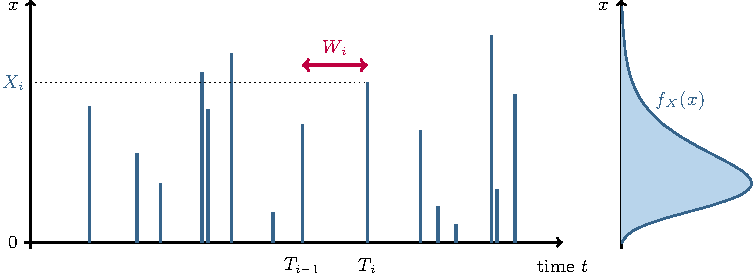
\includegraphics[width=12cm]{images/POT.pdf}
  \caption{\label{POT} Events and levels. The random variable.
    $W_i=T_i-T_{i-1}$ can be called interevent.}
\end{figure}

Under some general assumptions the times $T_i$ corresponding to
large enough levels $X_i$ should be well described by an
\textit{Homogeneous Poisson Process}.  Recall that for HPP events the
number $N$ of events on a time interval of length~$w$ has a Poisson
distribution with mean $\mu_N=\lambda \times w$. Moreover the numbers
of $T_i$ corresponding to disjoint intervals are independent.  The
parameter $\lambda>0$ is called the \textit{rate} 
\index{rate, Poisson process} and has the physical dimension of an inverse time: it will
generally be given in inverse years or events by year. Another
important property of the HPP is that the interevent random
variables~$W_i=T_i-T_{i-1}$ are independent with the same exponential
distribution with mean $1/\lambda$.  \index{interevent}


Unless explicitly stated otherwise, we will make the following
assumptions about the marked process.
\begin{enumerate}
\item Events $T_i$ occur according to a Homogeneous Poisson Process
  with rate $\lambda$.
\item Levels $X_i$ form a sequence of independent identically
  distributed random variables with continuous distribution
  function~$F_X(x)$, survival function $S_X(x)= 1-F_X(x)$ and density
  $f_X(x)$.
\item The levels sequence and events sequence are independent.
  \index{survival function}
\end{enumerate}
The distribution $F_X(x)$ will be chosen within a parametric family
and depends on a vector of parameters $\bs{\theta}_X$. This dependence
can be enlightened using the notation~$F_X(x;\,\bs{\theta}_X)$ when
needed, the same convention applying to the density and the survival
functions.  The survival function can often in POT be preferred to the
distribution function.  The parameters of the whole model consist in
$\lambda$ and a vector $\bs{\theta}_X$.


\subsection{Return period, return level}
%%---------------------------------------------
\label{RETPERLEV}
The \textit{return period} \index{return period!in POT} 
of a given level~$x$
is the mean time between two events $T_i$ with levels exceeding~$x$,
that is with $X_i > x$. Under the assumptions above, it is given by
\begin{equation}
  \label{eq:RETPER}
  T(x) = \frac{1}{\lambda \,S_X(x)}.
\end{equation}
Indeed the probability of $\{X_i>x\}$ is $S_X(x)$, and the events
with level exceeding~$x$ also form an HPP\footnote{The is due to the
  independence of the two sequences $X_i$ and $T_i$.}  (thinned HPP)
with rate $\lambda \,S_X(x) $.  
\index{thinning (Poisson Process)}%
The mean interevent is the inverse rate.

Conversely, for a given period $T>0$ the \textit{return level} $x(T)$
is the level value $x$ having the return period $T$. It is given by
\begin{equation}
  \label{eq:RETLEV}
  x(T) = q_X(p),\quad p := 1 - \frac{1}{\lambda T}
\end{equation}
\index{return level!in POT}%
\noindent
where $q_X$ is the quantile function. The period $T$ must be greater
than $1/\lambda$. The limit of $x(T)$ for large periods is the upper
end-point of the distribution, which can be finite in some cases.
\index{end-point} 

In practice, the interest is often focused only on
large return levels or periods.


\subsection{Peaks Over Threshold  (POT)}
%%-------------------------------------
\index{POT (Peaks Over Threshold)|(}

\subsubsection*{The POT framework}
%%---------------------------------------
In the POT approach, only the upper part of the distribution $F_X(x)$
is modelled. More precisely, the interest is on the part $X > u$ where
$u$ is a \textit{threshold}.  The steps are 

\index{threshold!in POT}

\begin{list}{$\bullet$}{
  \setlength{\itemsep}{0pt} 
  \setlength{\topsep}{2pt}
  }
\item Fix a suitable threshold $u$,
\item Consider only the observations with level $X_i$ greater than $u$
  i.e. with $X_i>u$,
\item Estimate the rate of the events $X_i>u$ and fit a distribution 
  for the \textit{excesses} $Y_i = X_i -u$.
  \index{excess}
\end{list}
The distribution of $X$ conditional on $X>u$ is deduced from that of
the excess~$Y$ by translation.

\begin{figure}
  \centering
  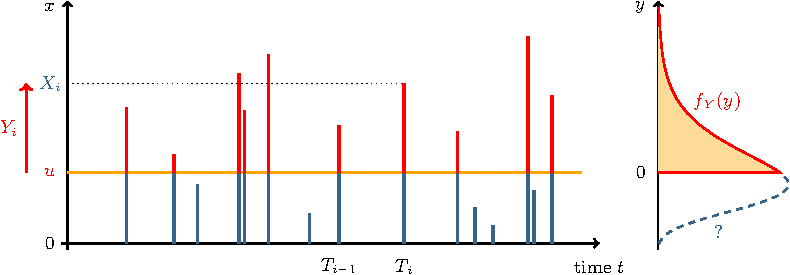
\includegraphics[width=12cm]{images/POTu.pdf}
  \caption{\label{POTu} In POT, only the levels $X_i$ with $X_i>u$
    are modeled through the excesses $Y_i=X_i-u$. The lower part $x <u$
    of the distribution $F_X(x)$ remains unknown.}
\end{figure}

The threshold will often be chosen above the mode of~$X$, leading to a
decreasing density for the excess~$Y$ as suggested on
figure~\ref{POTu}. The distribution of $Y$ typically has two
parameters.

\subsubsection*{Generalised Pareto Distribution}
%%----------------------------------------
The POT approach usually retains a GPD for the excess $Y$ or
equivalently a GPD for the level $X$ conditional on the exceedance $X
> u$. This choice is supported for a large threshold~$u$ by the
Pickands-Balkema-de Haan theorem
\index{Pickands-Balkema-de~Haan~theorem} (see~\ref{GEVGPD}) or by the
related \textit{POT-stability} property of the GPD
(see~\ref{GPDPROP}).  \index{POT stability} The family of GPDs with a
given shape parameter $\xi$ can be said to be POT-stable: if for a
given threshold $u$ the distribution of $X$ conditional on $X >u$ is a
GPD with shape $\xi$, then for any another threshold $v>u$ the
distribution of $X$ conditional on $X>v$ is still a GPD with the same
shape~$\xi$.  By selecting a threshold $v > u$ in POT, the estimation
will use a smaller set of $X_i$ but the underlying distribution of $X$
conditional on exceedance is the same in the two cases.
\index{exceedance}

\index{threshold!choice}
The choice of the threshold is a well-known difficulty in
classical POT where only GPD excesses are used~\citep{DAVSMITH}. 
The situation is much more complex with non-GPD excesses, because POT
stability no longer holds.
%% The family of GPDs with a given
%% shape parameter $\xi$ can be said "POT stable".  \index{POT stability}
%% With another threshold $v>u$ the estimation will use a smaller set of
%% $X_i$ but the underlying distribution of $X$ conditional on $X > v$ is
%% the same in the two cases.  
For instance if the excesses over
$u$ are Weibull with shape $\alpha>0$ and scale~$\beta = 1$ i.e.
$$
   \Pr\left\{\Cond{X>x}{X>u} \right\} =  \exp\left\{ - (x-u)^\alpha \right\} 
   \qquad x > u
$$
\index{Weibull distribution}%
%% then the conditional distribution over a higher threshold $v>u$ is
%% given by
%% $$
%%    \Pr\left\{\Cond{X>x}{X>v} \right\} = 
%% \exp\left\{ - \left[ (x-u)^\alpha -(v-u)^\alpha \right]\right\}   \qquad x > v > u
%% $$
then the conditional distribution of the excess $\Cond{X-v}{X>v}$ \textit{is not}
Weibull; it is a shifted version of the \index{left truncated Weibull}
\textit{Left Truncated Weibull} (LTW), see~\ref{SLTW}.

\index{POT (Peaks Over Threshold)|)}

\subsection{Link with Block Maxima}
%%---------------------------------------------
\index{block maxima|(} \index{rlargest@{$r$~largest}|(}%
\index{blocks}%

Alternative approaches to POT for univariate Extreme Values modelling
use time \textit{blocks} 
of, say, one year and related by-block data. Numerous
observations of the variable of interest $X$ are assumed to exist in
each block, and only the largest of them are retained in the
analysis. Popular examples are

\begin{list}{$\bullet$}{\setlength{\itemsep}{2pt}\setlength{\topsep}{2pt}}
  
\item \textbf{block maxima}: for each block, only the maximal value is
  used in the analysis.

\item \textbf{ $r$~largest}: for each block the largest~$r$
  observations (i.e. the $r$ largest order statistics) are recorded.
  The number~$r$ may vary across the blocks.  

\end{list}
Block maxima is the special case of $r$~largest for $r=1$, and using
$r>1$ largest observations when available leads to a better
estimation. The $r$~largest analysis is described in chap.~3 of the
book of \citet{COLES}. The distribution retained for the maxima or the
$r$~largest is based on asymptotic considerations. The block maxima
are usually assumed independent and to follow a Generalised Extreme
Value (GEV) distribution. From the Fisher-Tippett-Gnedenko theorem, 
this corresponds to the situation where $n$
independent and identically distributed $X_i$ are found in each block,
the number~$n$ being large --~see section~\ref{ASYMPTGEV}.



%% Underlying the block data, one would generally find a continuous time
%% process (e.g. temperature, sea surge), possibly observed at fixed
%% times (e.g. high tide). The time-length of the blocks is generally
%% chosen in order to reach a limit behaviour ignoring autocorrelation or
%% seasonality in the continuous process.

\begin{figure}
  \centering
  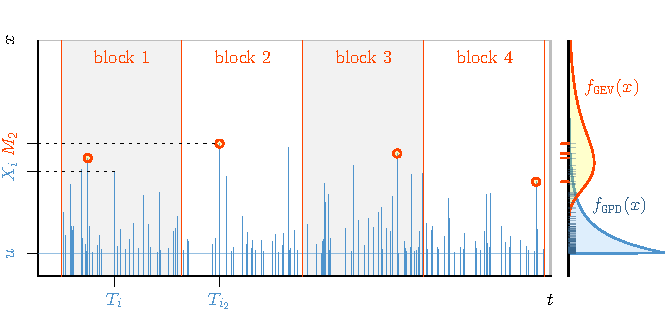
\includegraphics[width=12cm]{images/RenouvAgc.pdf}
  \caption{\label{RenouvAg} Block maxima for the marked
    process. If the marks $X_i$ follow a GPD, then for a constant block duration
    the block maxima $M_b:=X_{i_b}$ follow a GEV distribution
    (provided that they exist).  
  }
\end{figure}

Interestingly, the assumptions concerning the marked point process as
stated before in~\ref{ASSUMPTIONS} provide a framework to derive the
distribution of the maxima or that of the $r$~largest observations
over non-overlapping blocks, without any asymptotic consideration.
Given $B$ such blocks $b=1$, $2$, $\dots$, $B$ with known duration~$w_b$, 
the maximum $M_b$ for block $b$ is the maximum of $N_b$ levels
$X_i$ with $T_i$ falling in that block, where $N_b$ has a Poisson
distribution with mean $\lambda w_b$.  Moreover the maxima $M_b$ are
independent across blocks. The distribution of the $M_b$ can be
related to the distribution of the marks: see appendix
page~\pageref{COMPOUND}.  Note however that the marked process can
lead to blocks $b$ with no observation, especially when the block
duration $w_b$ is not large relative to the mean interevent
$1/\lambda$.  Similarly, the joint distribution of the $r$~largest in
a block is easily derived, see section~\ref{SECHISTORY} later.

When the distribution of the marks $X_i$ is assumed to be GPD and the
blocks have the same duration $w_1$ (e.g. one year), the block maxima
$M_b$ are independent and follow a GEV distribution, as is usually
assumed for block maxima. It can be shown as well that the
distribution of the $r$~largest observations $X_i$ is then the distribution
used in the $r$~largest analysis Coles~\citep[chap.~3]{COLES},
provided that at least $r$ observations~$X_i$ exist. The notion of
\emph{return period} for the blocks framework differs from the one
given above see discussion~\ref{TWORL} page~\pageref{TWORL}.  However,
the difference between the two notions is confined to the small return
periods context.

To summarise:  maxima or $r$~largest observations can be viewed as
\textit{partial observations} \index{partial observation} of the
marked process, or as the result of a \textit{temporal aggregation}
\index{aggregation, temporal} of this process. When the result of such
an aggregation (i.e.  maxima or $r$~largest) is known for one or
several blocks with large duration, say decades or centuries, we may
speak of \textit{historical data}.  
\index{historical data}%

Although \textbf{Renext} primarily uses the original data
$[T_i,\,X_i]$ as described in~\ref{ASSUMPTIONS} above, it is possible
to make use of supplementary block data in a quite flexible
fashion. Maxima and $r$~largest observations within block(s) can also
be used, as well as the marks exceeding some known auxiliary threshold
as sometimes called a \textit{perception threshold}. A typical use of
these possibilities is for historical data.
\index{threshold!perception}%
\index{block maxima|)}
\index{rlargest@{$r$~largest}|)}%

\subsection{Declustering}
%%--------------------------------
\index{declustering}
Most of Extreme Values problems concern a continuous time process:
discharge flow, temperature, sea surge, etc.
POT modelling most often requires a \textit{declustering} step leading to
independent events: floods, heat or cold waves,
storms, etc. \pkg{Renext} does not currently provide any declustering
function, which can be found in the other POT packages cited above. 



\section{Heterogeneous data}
%%==============
\subsection{Remarks}
%%-----------------
Model fitting functions in~R usually have a formal argument specifying
data with a \textit{data frame} object, the model being typically
given by a \textit{formula}. Due to the presence of heterogeneous
types of data within a given ``dataset'', the arguments of
\textbf{Renext} functions will take a slightly more complex form. For
instance, it will generally be necessary to specify a duration or
several block durations in complement to the vector of levels, to specify
where missing periods (gaps) occurred, etc.

Some of the package functions require the use of \verb@POSIX@ objects
representing date and time. R~base package provides versatile
functions to manage date/time or timestamps. See for instance the help
of the \verb@strptime@ function.  
\index{POSIX objects@{\texttt{POSIX} objects}}

As most R~packages do, \textbf{Renext} comes with a few datasets taken
from relevant literature or from real data examples. These datasets
are given as lists objects with hopefully understandable element
names. Some datasets have an S3 class named \verb@"Rendata"@ and can
as such be used as the first formal argument of popular S3 methods: 
\verb@plot@, \verb@summary@ and more.

\subsection{OT data}
%%-----------------
\index{OTdata@{\texttt{OTdata}}|(}% 

The data used in POT will mainly consist in recorded levels $X_i$ or
levels exceeding a reasonably low known threshold~$u_\star$, with possibly
$u_\star=-\infty$. Such data will be called \textit{OT data} for
``Over Threshold''. The POT modelling will typically use a higher
suitably chosen threshold $u>u_\star$.

\index{Brest data@{\texttt{Brest} data}|(}
The data \verb@Brest@ contain sea surge heights at high
tide for the Brest gauging station. Only values exceeding $u_\star=30$\,cm
are retained. More details about these data are provided in the
package manual. The data are provided as a list with several parts.

\begin{Schunk}
\begin{Sinput}
> library(Renext)
> names(Brest)
\end{Sinput}
\begin{Soutput}
[1] "info"      "describe"  "OTinfo"    "OTdata"    "OTmissing"
\end{Soutput}
\end{Schunk}

\noindent
As their names may suggest the list elements contain Over Threshold
(OT) data and information.

\begin{Schunk}
\begin{Sinput}
> head(Brest$OTdata, n = 4)
\end{Sinput}
\begin{Soutput}
        date  Surge comment
1 1846-01-14 35.989        
2 1846-01-21 59.987        
3 1846-01-24 45.986        
4 1846-01-28 39.985        
\end{Soutput}
\begin{Sinput}
> str(Brest$OTinfo)
\end{Sinput}
\begin{Soutput}
List of 4
 $ start      : POSIXct[1:1], format: "1846-01-01"
 $ end        : POSIXct[1:1], format: "2009-01-01"
 $ effDuration: num 148
 $ threshold  : num 30
\end{Soutput}
\end{Schunk}

\noindent
The \verb@OTdata@ element is a data frame giving the $T_i$ (in time
order) and the corresponding levels~$X_i$.  Note that the time part of
the \verb@POSIX@ object may not be relevant. Here only the date part
makes sense and the time part is by convention \verb@"00:00"@ with the
time zone set to \verb@"GMT"@ to use Coordinated Universal Time (UTC).
Of course, the observations were made at a different time.
\index{Coordinated Universal Time (UTC)}

%% However
%% on such a large period of time, it can be affected by \textit{leap seconds}, and
%% \verb@"00:00"@ might appear as \verb@"23:59"@ the day
%% before. 
%% \index{leap seconds}%

The \verb@OTinfo@ list mentions an \textit{effective duration}. This
is less than the time range which can be computed using the methods
\verb@range@ and \verb@diff@ from the \textbf{base} package
%% ## as.numeric(diff(range(Brest$OTdata$date), units= "days"))/365.25

\begin{Schunk}
\begin{Sinput}
> End <- Brest$OTinfo$end; Start <- Brest$OTinfo$start
> Dur <- as.numeric(difftime(End,  Start, units = "days"))/365.25
> Dur
\end{Sinput}
\begin{Soutput}
[1] 162.9979
\end{Soutput}
\begin{Sinput}
> Dur - as.numeric(Brest$OTinfo$effDuration) 
\end{Sinput}
\begin{Soutput}
[1] 15.37795
\end{Soutput}
\end{Schunk}

\noindent
The difference --~more than 15 
years~-- is due to gaps or \textit{missing periods}. 
\index{missing periods!description}%
The missing periods are described in the element \verb@OTmissing@.
%%The \verb@MAXdata@ and \verb@MAXinfo@ are here \verb@NULL@ but could 
%%contain data as in \verb@Garonne@ example described below.

The \verb@Brest@ dataset has class \verb@"Rendata"@. This is an S3 
class defined in \textbf{Renext} to describe objects containing
\verb@OTdata@ and possibly some extra information on missing periods
or historical data. It has a \verb@summary@ method 
\index{Rendata class@{\texttt{Rendata} class}|(}

\begin{Schunk}
\begin{Sinput}
> class(Brest)
\end{Sinput}
\begin{Soutput}
[1] "Rendata"
\end{Soutput}
\begin{Sinput}
> summary(Brest)
\end{Sinput}
\begin{Soutput}
o Dataset Surge Heights at Brest (France)
   data 'Brest', variable 'Surge' (cm) 

o OT data (main sample) from  1846-01-01  to  2009-01-01  (eff. dur. 147.62 years)
 
         n       Min.    1st Qu.     Median       Mean    3rd Qu.       Max. 
1289.00000   30.02200   33.64700   38.30600   41.76007   46.58100  143.94900 

o missing 'OT' periods, total 15.38 years 

           n         Min.      1st Qu.       Median         Mean      3rd Qu. 
43.000000000  0.002737851  0.016427105  0.038329911  0.357639718  0.086242300 
        Max. 
 8.418891170 

o no 'MAX' historical data 

o no 'OTS' historical data 
\end{Soutput}
\end{Schunk}

\noindent
The displayed information concerns the levels in the main OT sample
and the possible gaps in this sample: number, duration (in years).
A \verb@plot@ method also exists

\begin{Schunk}
\begin{Sinput}
> plot(Brest)
\end{Sinput}
\end{Schunk}

\noindent
which produces the plot on the left of figure~\ref{RENPLOTS}.

\index{Brest data@{\texttt{Brest} data}|)}
\index{OTdata@{\texttt{OTdata}}|)}%

\subsection{Missing periods or gaps}
%%--------------------------------
\index{missing periods!description}% 
\index{gaps|see{missing periods}}%
A common problem in POT modelling is the existence of gaps within the
observation period. These can result from many causes: damage or
failure of the measurement system, human errors, strikes, wars, ...

\textbf{Renext} uses a natural description of the gaps within a
dataset. They are stored as rows of a data.frame with two \verb@POSIX@
columns \verb@start@ and \verb@end@

\begin{Schunk}
\begin{Sinput}
> head(Brest$OTmissing, n = 4)
\end{Sinput}
\begin{Soutput}
       start        end comment
1 1846-01-01 1846-01-04        
2 1847-01-01 1847-01-21        
3 1852-01-21 1852-02-08        
4 1857-05-31 1859-11-24        
\end{Soutput}
\end{Schunk}

\noindent
Missing periods must be taken into account in the analysis. They
should be displayed on timeplots showing events, since it is
important to make a distinction between periods with no events and
gaps, see figure~\ref{RENPLOTS}. An important prerequisite to modelling
is to ensure that the gaps occur independently from measured
variables. For instance, storms can damage gauging systems for wind or
sea level thus leading to \textit{endogenously missing} observations forming an 
endogenous gap. This may be considered as a form of censoring.

\index{missing periods!endogenous}
\index{censoring}

\subsection{Aggregated (block) data}
%%------------------------
\index{historical data}% 
\label{HistoricalData}
\index{block data|(}%

\subsubsection*{Motivation}
%%-------------------------
In a \verb@Rendata@ object, the ordinary data provided in the
\verb@OTdata@ element can be completed by some data observed in
blocks with known duration. This possibility is often
required to use historical information.  Two types of block data are
currently supported under the names "MAX" and "OTS" data.  These 
can be regarded as the two types of censored data: type~I
for OTS and type~II for MAX, and are described more precisely
in section~\ref{TwoTypes}
page~\pageref{TwoTypes}.

\subsubsection*{MAXdata}
%%----------------------------
\index{MAXdata@{\texttt{MAXdata}}}%
As a first possible complement to \verb@OTdata@, we may have \verb@MAXdata@ that
is: $r$~largest observations over one or several blocks. Such
data require a complementary information: the block duration(s) which
must be given in years.

\index{Garonne data@{\texttt{Garonne} data}|(}
The dataset \verb@Garonne@ is taken from~\citet{MIQUELBOOK} where
it is described.  The data concern the french river \textit{La
  Garonne} at the gauging station named \textit{Le Mas d'Agenais}
where many floods occurred during the past centuries.  The data
consist in both OT data and historical data. The variable is the river
discharge flow in $\textrm{m}^3/\textrm{s}$ as estimated from the river level
using a rating curve. The precision is limited and many ties are
present among the flow values.  The OT data contain flow values over
the threshold $u = 2500~\textrm{m}^3/\textrm{s}$. 

The historical data in \verb@Garonne@ are simply the~$12$ largest
flows for a period of about $143$~years and will be used later.

\begin{Schunk}
\begin{Sinput}
> names(Garonne)
\end{Sinput}
\begin{Soutput}
[1] "info"      "describe"  "OTinfo"    "OTdata"    "OTmissing" "MAXinfo"  
[7] "MAXdata"  
\end{Soutput}
\begin{Sinput}
> Garonne$MAXinfo
\end{Sinput}
\begin{Soutput}
       start        end duration
1 1770-01-01 1913-01-01   143.09
\end{Soutput}
\begin{Sinput}
> head(Garonne$MAXdata, n = 4)
\end{Sinput}
\begin{Soutput}
  block date Flow  comment
1     1 <NA> 7500 1 (1875)
2     1 <NA> 7400 2 (1770)
3     1 <NA> 7000 3 (1783)
4     1 <NA> 7000 4 (1855)
\end{Soutput}
\end{Schunk}

\noindent
The \verb@Garonne@ dataset has class \verb@"Rendata"@. The \verb@plot@
method for this class

\begin{Schunk}
\begin{Sinput}
> plot(Garonne)
\end{Sinput}
\end{Schunk}

\noindent
produces a graphic displaying the historical period as on the right
panel of figure~\ref{RENPLOTS}. Here the dates of the historical
events are not known exactly and thus are provided here as \verb@NA@
\verb@POSIXct@ objects. The historical levels are thus displayed as
horizontal segments, while vertical segments would be used for known
dates.  The \verb@plot@ method for the class \verb@Rendata@ has a
\verb@showHist@ logical formal argument telling that historical
periods should be shown (default value \verb@TRUE@) or not.


Note that the function \texttt{OT2MAX} can be used to compute the
$r$~largest values in blocks of one year from observations
$[T_i,\,X_i]$ of a marked process. This function can be used to
compare a POT approach to block maxima or $r$~largest,
see~\ref{OT2MAX}.

\begin{figure}
   \centering
   \begin{tabular}{c c} 
     \includegraphics[width=7cm]{Rgraphics/fig-RenplotBrest.pdf} &
     \includegraphics[width=7cm]{Rgraphics/fig-RenplotGaronne.pdf} 
   \end{tabular}
   \caption{\label{RENPLOTS} Graphics produced using the \texttt{plot}
     method of the \texttt{"Rendata"} class. On the left, the
     \texttt{Brest} object contains missing periods that are shown.
     On the right, the \texttt{Garonne} dataset contains information
     about an \textit{historical period}, displayed as a green rectangle.  }
\end{figure}
\index{Garonne data@{\texttt{Garonne} data}|)}

It can be remarked here that working with the original unit leads to
observations with a quite large order of magnitude. This can be a
problem in some numerical evaluations such as the determination of a
hessian.  \index{hessian} Although the \verb@Renouv@ function used
later internally scales the data, it could be preferable to rescale
the data e.g. by dividing them by $1000$.
\index{rescaling (data)}
\index{scale of data|see{rescaling (data)}}

\subsubsection*{OTSdata}
%%----------------------------
\index{OTSdata@{\texttt{OTSdata}}}%

The other type of block data involves a number of $B$ non-overlapping
blocks.  For each block $b=1$, $2$, $\dots$, $B$ the duration $w_b$ is
assumed to be known as well as a threshold $u_b$. We then assume to be
given all the observations with level $X_i$ exceeding the threshold
$u_b$ i.e. with $X_i > u_b$.  It is assumed that no OTS threshold
$u_b$ is smaller than the OT threshold~$u$. In some cases the
times $T_i$ are known and can be provided in the \verb@date@ column
of the data frame \verb@OTSdata@.  Unlike with \verb@MAXdata@, one
block can be empty because no level $X_i$ exceeding $u_b$ was
found. The block will then appear in the \verb@OTSinfo@ data frame
but not in~\verb@OTSdata@.

\subsection{Overview}

The general structure of a \verb@Rendata@ object is described in
table~\ref{RENDATATAB}.

\begin{table}
  \centering
  \begin{tabular}{l l l }
    \toprule
    \multicolumn{1}{c}{element} & 
    \multicolumn{1}{c}{class} & 
    \multicolumn{1}{c}{content} \\ \toprule
    \texttt{info} $(\star)$   & \texttt{list}     & 
    general information: variable name, units, ...
    \\
    \texttt{describe}       & \texttt{character}  & optional description\\  \hline
    \texttt{OTinfo} $(\star)$ & \texttt{list}     & 
    \texttt{start}, \texttt{end}, \texttt{duration} $w$, \texttt{threshold} $u$\\
    \texttt{OTdata} $(\star)$ & \texttt{data frame} & 
    \texttt{date} $T_i$, \textit{level} $X_i$ and \texttt{comment} \\
    \texttt{OTMissing}      & \texttt{data frame} & 
     \texttt{start}, \texttt{end}, \texttt{comment} \\ \hline 
    \texttt{MAXinfo}        & \texttt{data frame} & 
    \texttt{start}, \texttt{end}, \texttt{duration} $w_b$\\
    \texttt{MAXdata}        & \texttt{data frame} & 
    \texttt{block}, \texttt{date}, \textit{level}, \texttt{comment}\\ \hline
    \texttt{OTSinfo}        & \texttt{data frame} & 
    \texttt{start}, \texttt{end}, \texttt{duration} $w_b$, \texttt{threshold} $u_b$
    \\
    \texttt{OTSdata}        & \texttt{data frame} & 
    \texttt{block}, \texttt{date}, \textit{level}, \texttt{comment}\\ \toprule
  \end{tabular}
  \caption{\label{RENDATATAB}
    Structure of a \texttt{Rendata} object. The required elements are marked 
    with a star $(\star)$. The threshold in \texttt{OTinfo} can be set to \texttt{-Inf},
    thus allowing the computations of the excesses $X - u$ for any threshold $u$.}
    
\end{table}

The \verb@readXML@ function (still experimental) can be used to read
such heterogeneous data from an XML file and possibly linking to csv files. Some
examples are shipped with the package, see help with \verb@?readXML@.
\index{XML}
\index{readXML function@{\texttt{readXML} function}}
  
\subsection{Simulating heterogeneous data}
%%-------------------------------
\index{simulation} 
\index{rRendata function@{\texttt{rRendata} function}|(}
Heterogeneous data generated by a Monte-Carlo simulation are of great
help in POT-based analysis. For instance, simulated data can be used
to assess the bias of an estimate, or to compare several plotting
positions. It also helps in getting familiar with the random
variations in the estimates or in the return level plots.  The
\verb@rRendata@ function can be used to generate a \verb@RenData@
object with a specific design: duration of the main sample, number and
durations of MAX data or OTS blocks.

Suppose that we use a main sample of (default) duration $100$ years
and the default distribution the standard exponential. We can enhance
the data by adding three MAX blocks of say $40$, $50$ and $30$
years. By default, only the maximum observation will be kept in each
block.

\begin{Schunk}
\begin{Sinput}
> set.seed(1234)
> RD1 <- rRendata(MAX.effDuration = c(40, 50, 30))
> plot(RD1)
\end{Sinput}
\end{Schunk}

\noindent
See left of figure~\ref{RRENDATA}. The three MAX blocks are by
convention located before the start of the main sample since in
practice such blocks often represent historical data. We can similarly
add $3$ OTS blocks with $3$ choosen durations and thresholds.

\begin{Schunk}
\begin{Sinput}
> RD2 <- rRendata(effDuration = 30,
                  distname.y = "GPD",
                  par.y = c(scale = 1, shape = 0.1),
                  OTS.effDuration = c(40, 50, 30), OTS.threshold = c(3, 4, 2))
> plot(RD2)
\end{Sinput}
\end{Schunk}

\noindent
Note that we used here a non-default \texttt{"GPD"} distribution for
the excesses $Y_i$, and we gave the values of the parameters. For now,
the \verb@rRendata@ function can not generate random missing periods.

\begin{figure}
   \centering
   \begin{tabular}{c c} 
     \includegraphics[width=7cm]{Rgraphics/fig-rRendata1.pdf} &
     \includegraphics[width=7cm]{Rgraphics/fig-rRendata2.pdf} 
   \end{tabular}
   \caption{\label{RRENDATA} 
     Two randomly generated \texttt{Rendata}
     objects. The distribution of the marks is exponential on the
     left, and GPD on the right. Three MAX blocks are used on the 
     left, and three OTS blocks are used on the right.
   }
\end{figure}
\index{rRendata function@{\texttt{rRendata} function}|)}
\index{Rendata class@{\texttt{Rendata} class}|)}
\index{block data|)}%

\subsection{Aggregated  data and gaps} 
%%----------------------------------
A difficulty with aggregated data such as block data concerns the
treatment of missing data or gaps. There is usually no reason that
missing periods should correspond to full blocks (e.g. years), and
most often a fraction of some blocks is missing. Excluding all blocks
with missing data leads to a severe loss of information, while
ignoring gaps in blocks may cause a bias.  The use of aggregated data
will be illustrated later in the section~\ref{CountData}
about \verb@barplotRenouv@. The problem of gaps in blocks will be also be
discussed when describing the \verb@OT2MAX@ function in
section~\ref{OT2MAX} p.~\pageref{OT2MAX}.
  

\chapter{Descriptive  tools}
%%============================
\label{Chap-DescriptiveTools}

Some functions of \pkg{Renext} have been designed to check the
assumptions relative to the stationnarity of the events or to the
distribution of the levels.  The analysis of the events can cope with
gaps as are often met in practice. Although of less importance, the
case where counts are used in place of events is also considered.

\section{Functional plots}
%%---------------------------
\subsection{Principles}
%%----------------------------
\label{FUNCPLOTS}
\index{Gumbel plot}\index{exponential plot}%
Widespread graphical tools in statistics are \textit{functional
  plots}, such as exponential plot, Weibull or Gumbel plots. In all
cases, the plot is designed so that the theoretical distribution curve
(exponential/Weibull/Gumbel) shows as a straight line. For instance
the relations for distribution functions $F$
\begin{align*}
  -\log\left[1-F(x) \right] &= (x-\mu)/\sigma     \quad \textrm{(exponential)}\\
  \qquad
  -\log\left[-\log F(x) \right] &= (x-\mu)/\sigma \quad \textrm{(Gumbel)}
\end{align*}
both show a linear relation between $x$ and a transformed version
$\phi(F)$ of~$F(x)$, e.g. $\phi(F)= -\log\left[1-F \right]$ for the
exponential case.  The functional plots are obtained by plotting
$[x,\,\phi(F)]$ still using the values of the probability $F$ to
display the unevenly spaced graduations on the $y$-axis. The Weibull
plot is similar but also uses a (log) transformation of~$x$.

With a sample $X_i$ of size $n$ one uses non-parametric estimates
$\widetilde{F}_i$ of the values $F(Z_{i})$ of the distribution
function at the order statistics $Z_{i}$ with $Z_1> Z_2 > \dots >
Z_n$. The~$n$ resulting points with ordinates $\widetilde{F}_{i}$ can
be plotted with the transformed scale on the $y$-axis. A classical
choice for the plotting positions is implemented in the \verb@ppoints@
function of the \pkg{stats} package \index{plotting positions}%
\begin{equation}
  \label{eq:CUNNAME}
  \widetilde{F}(Z_{n+1-i}) = \frac{i-a}{n -2a + 1},
\end{equation}
where $a$ is a parameter typically in the interval $[0,\,1]$.  The
right hand side is the expectation of the random variable
$F(Z_{n+1-i})$ for $a=0$ and an approximation of its median for
$a=0.3$. 
\index{ppoints function@{\texttt{ppoints} function}}

As some other packages do, \textbf{Renext} provides exponential and
Weibull plotting functions, namely \verb@expplot@ and \verb@weibplot@

\begin{Schunk}
\begin{Sinput}
> expplot(x = Brest$OTdata$Surge, main = "expplot for \"Brest\"")
\end{Sinput}
\end{Schunk}
\vspace{-13pt}
\begin{Schunk}
\begin{Sinput}
> weibplot(x = Brest$OTdata$Surge-30, main = "weibplot for \"Brest\" (surge - 30)")
\end{Sinput}
\end{Schunk}

\noindent
producing the two plots on figure~\ref{FUNG}.

Note that the transformation $\phi(F)$ must not depend on unknown
parameters. Therefore the Weibull plot produces a theoretical line
only for the version with two parameters (shape and scale), and not
for the three parameter one (with location).
\begin{figure}
   \centering
   \begin{tabular}{c c} 
     \includegraphics[width=7cm]{Rgraphics/fig-exppBrest.pdf} &
     \includegraphics[width=7cm]{Rgraphics/fig-weibpBrest.pdf} 
   \end{tabular}
   \caption{\label{FUNG} Exponential and Weibull plot for the Brest
     data. The variable \texttt{Surge} is used for the exponential
     plot. The threshold $30$~cm is subtracted from \texttt{Surge} for
     the Weibull plot. The later uses a log-scale for \texttt{x}.  }
\end{figure}

\subsection{Exponential vs Gumbel}
%%---------------------------------

While hydrologists often favour Gumbel plots, the exponential plot may
also be used. The latter is better suited to the use of "OTdata"
i.e. data where only values over a threshold~$u$ are kept. Even if
the original observations $X_i$ are Gumbel, the conditional
distribution $\Cond{X_i}{X_i>u}$ will be close to an exponential for
$u$ large enough, see~\ref{GEVGPD}. This can be illustrated with a
few simple R commands \label{GUMBEXP}

\begin{Schunk}
\begin{Sinput}
> library(evd); set.seed(136)
> X <- rgumbel(400); X <- X[X > 0.6]           ## X is truncated Gumbel
> n <- length(X); 
> Zrev <- sort(X); F <- (1:n) / (n + 1)           ## distribution function
> y.exp <- -log(1 - F); y.gum <- -log(-log(F))   
> plot(Zrev, y.exp, col = "red3", main = "exponential plot")
\end{Sinput}
\end{Schunk}
\vspace{-13pt}
\begin{Schunk}
\begin{Sinput}
> plot(Zrev, y.gum, col = "SteelBlue3", main = "Gumbel plot")
\end{Sinput}
\end{Schunk}

\noindent
The two plots are shown on figure~\ref{EXPGUM}. The difference
between exponential and Gumbel plots is restricted to the small values.

\begin{figure}
   \centering
   \begin{tabular}{c c} 
     \includegraphics[width=7cm]{Rgraphics/fig-ExpPlot.pdf} &
     \includegraphics[width=7cm]{Rgraphics/fig-GumPlot.pdf} 
   \end{tabular}
   \caption{\label{EXPGUM} Truncated or "thresholded" Gumbel random
     sample.  Due to the truncation, the sample distribution is close
     to an exponential.  The graduations for the $y$-axis are not in
     probability-scale.}
\end{figure}

\section{Events and stationarity}
%%===================================

\subsection{Simple plots}
%%---------------------------
The simplest plot for checking stationarity has points $[T_i, \, X_i]$
and can be obtained with R~functions of the \verb@graphics@
package. The $T_i$ and $X_i$ will typically be available as two
vectors of the same length or as two columns of a same data.frame
object. For the example datasets of \textbf{Renext}, the $T_i$ and
$X_i$ are given as two columns of the \verb@OTdata@ data frame

\begin{Schunk}
\begin{Sinput}
> plot(Flow ~ date, data = Garonne$OTdata, type = "h", main = "Flows > 2500 m3/s")
\end{Sinput}
\end{Schunk}

\noindent
The graphic shows that several successive years had no exceedance
over $2500~\textrm{m}^3/\textrm{s}$ during the second half of the
1940-1950 decade. This could lead to further investigations using the
\verb@subset@ function

\begin{Schunk}
\begin{Sinput}
> subset(Garonne$OTdata, date >= as.POSIXct("1945-01-01") & date <= as.POSIXct("1950-01-01"))
\end{Sinput}
\begin{Soutput}
         date Flow comment
96 1945-01-29 3200        
\end{Soutput}
\end{Schunk}

\index{subset method@{\texttt{subset} method}}

\noindent
The graphics can be enhanced using the \verb@text@ function in the
\verb@graphics@ package to annotate special events or periods.

\begin{figure}
   \centering
   \begin{tabular}{c c} 
     \includegraphics[width=7cm]{Rgraphics/fig-spGaronne.pdf} & 
   \end{tabular}
   \caption{\label{SpGar} Simple plot of events for the \texttt{Garonne} data.}
\end{figure}

\subsection{Uniformity}
%-------------------------
The \verb@gof.date@ function performs some tests to check the
(conditional) uniformity of the events $T_i$ as implied by the HPP
assumption. It is based on the fact that for a given interval of time
$(s,\,t)$ the events $T_i$ falling in the interval are jointly
distributed as are the order statistics of a sample of the uniform
distribution on $(s,\,t)$. The sample size~$n$ is then
random. Alternatively, the $n$ events falling in an interval
$(T_k,\,T_{n+k+1})$ also have this joint conditional distribution. In
both cases a Kolmogorov-Smirnov (KS) test is well suited to check the
uniformity.
\index{Kolmogorov-Smirnov test}

The \verb@gof.date@ function mainly works with a \verb@POSIX@ object
containing the events~$T_i$ as in

\begin{Schunk}
\begin{Sinput}
> gof.date(date = Garonne$OTdata$date)
\end{Sinput}
\end{Schunk}

\noindent
which produces the plot on the left of figure~\ref{KSEVT}. The
empirical cumulative distribution function (ECDF) is compared to the
uniform and the KS distance $D_n$ is shown as a vertical segment.
The displayed KS $p$-value tells that uniformity should be rejected at
the significance level of $0.1\%$. Though less clearly than above, the
plot points out that the years 1940-1950 had fewer events.

The \verb@gof.date@ function has optional args \verb@start@ and
\verb@end@ to specify (and possibly restrict) the period on which the 
test is performed.
By default these are taken as the first and last event in \verb@date@
and therefore only inner events are used in the ECDF.

\subsection{Interevents}
%-------------------------
\index{interevent|(}% 
An important property of the HPP concerns the interevents 
$W_i = T_i-T_{i-1}$: the $W_i$ are independent and have exponential 
distribution 
\index{exponential distribution}%
with rate~$\lambda$. Thus an exponentiality test might be performed
to check the HPP assumption for observed data.

The \verb@interevt@ function computes the interevents $W_i$ as numbers of days. The
function returns a list with a \verb@interevt@ data.frame element containing
the $W_i$ in the \verb@duration@ column which can be used to check exponentiality.
This can be done either with a plot -~see figure~\ref{KSEVT} or 
with the test of exponentiality  of the function \verb@gofExp.test@
%%Since these are of class \verb@"difftime"@, they must be coerced 
%%to numeric before using exponential plot or a test.

\begin{Schunk}
\begin{Sinput}
> ie <- interevt(date = Garonne$OTdata$date)
> names(ie)
\end{Sinput}
\begin{Soutput}
[1] "interevt" "noskip"  
\end{Soutput}
\begin{Sinput}
> d <- ie$interevt$duration
> expplot(d, main = "Exponential plot for interevents")
> bt <- gofExp.test(d) 
> bt
\end{Sinput}
\begin{Soutput}
$statistic
[1] 193.9517

$df
[1] 149

$p.value
[1] 0.01560322

$method
[1] "Bartlett gof for exponential"
\end{Soutput}
\end{Schunk}

\noindent
It seems unlikely to obtain a good exponential fit
as far as events occurrence shows seasonality as is the case here.
A seasonality can no longer result from another distribution of 
interevents --~that is from a non-Poisson stationary renewal process.
Increasing the threshold might improve the adequacy with the 
assumptions.

\begin{figure}
  \centering
  \begin{tabular}{c c} 
    \includegraphics[width=8cm]{Rgraphics/fig-gdGaronne.pdf} &
    \includegraphics[width=8cm]{Rgraphics/fig-ieGaronne.pdf} 
  \end{tabular}
  \caption{\label{KSEVT} Analysis of the events for the
    \texttt{Garonne} data set (OTdata).  Left panel: test for the
    uniformity of events with the KS distance shown as a
    vertical segment.  Right panel : exponential plot for the
    interevents.}
\end{figure}
\index{interevent|)}

\subsection{Missing periods or gaps}
%%---------------------------------
\index{missing periods!in interevents}% 
In practice the situation is somewhat more
complex due to the possible existence of missing (or skipped) periods
where no events have been recorded.  Event rates should then be
computed using \textit{effective duration} 
\index{effective duration}%
that is: the total duration of measurement \textit{ignoring missing
  periods}.

The functions \verb@gof.date@ and \verb@interevt@ can take this
problem into consideration. The \verb@gof.date@ plot can display the
missing periods or "gaps" provided that a suitable \verb@skip@ arg is
given. For instance the following commands produce the plot on the
left of figure \ref{gofBREST}

\begin{Schunk}
\begin{Sinput}
> gof.Brest  <- gof.date(date = Brest$OTdata$date, skip = Brest$OTmissing,
                         start = Brest$OTinfo$start, end = Brest$OTinfo$end)
> print(names(gof.Brest))
\end{Sinput}
\begin{Soutput}
 [1] "effKS.statistic" "effKS.pvalue"    "KS.statistic"    "KS.pvalue"      
 [5] "effnevt"         "nevt"            "rate"            "effrate"        
 [9] "duration"        "effduration"     "noskip"         
\end{Soutput}
\end{Schunk}

\noindent
As their name may suggest, the returned list elements give the
effective duration 
\index{effective duration}%
and the effective rate based on the true non-missing periods. The 
\verb@noskip@ element contains detailed information about each non-skipped
period

\begin{Schunk}
\begin{Sinput}
> head(gof.Brest$noskip, n = 2)
\end{Sinput}
\begin{Soutput}
       start        end duration nevt      rate        Dn         KS
1 1846-01-04 1847-01-01 0.991102   17 17.152624 0.2586935 0.17172882
2 1847-01-21 1852-01-21 4.999316   48  9.601314 0.2057777 0.02929104
\end{Soutput}
\end{Schunk}

\noindent
For each period the rate has been computed as well as a KS test of
uniformity.  The power of the test is obviously limited for periods
containing only a few events.  \index{Kolmogorov-Smirnov test}

The preceding call to \verb@gof.date@ corresponded to the default
value of \verb@plot.type@, namely \verb@"skip"@. A drawback of the plot
and KS test is that the comparison with the uniform is biased by the
gaps.  The KS distance~$D_n$ between the empirical and theoretical
distributions can be amplified by the gaps when there are too few
events or, on the contrary, be reduced by gaps when there are too much
events. These two phenomena can be seen by comparing the two plots of
figure~\ref{gofBREST} although the two KS statistics and $p$-value are
here nearly identical. The right panel plot was produced using the
non-default choice for the \verb@plot.type@ arg i.e.  
\verb@plot.type= "omit"@, missing periods can be omitted on the plot and in the KS
test computation.

\begin{Schunk}
\begin{Sinput}
> gof.Brest2  <- gof.date(date = Brest$OTdata$date, 
                          skip = Brest$OTmissing, plot.type = "omit",
                          start = Brest$OTinfo$start, end = Brest$OTinfo$end)
\end{Sinput}
\end{Schunk}

\noindent
The time axis now has \textit{unevenly} spaced ticks since it is
obtained by concatenating the successive non-missing periods. More
precisely, each retained time interval $k$ begins at the first event
$T_{f_k}$ of a continuous observation period and ends at its last
event $T_{\ell_k}$. Each of the vertical lines shows an
interval $(T_{\ell_k},\,T_{f_{k+1}})$, which covers a missing period
and is cut out as shown on figure~\ref{KSomit}.  The displayed
information on the right panel of figure~\ref{gofBREST} concerns
\verb@effKS.pvalue@ and \verb@effKS.statistic@ of an "effective" KS
test performed on non-missing periods.  Provided that observation gaps
occur independently from the events $T_i$, the interevents for couples
of successive events falling in the same non-missing period can be
used in a modified KS test. In the HPP case, these interevents should
be independent and identically distributed with exponential
distribution, thus concatenating them should produce an HPP hence an
uniform conditional distribution of events.

For the \verb@Brest@ example, the test tells us that the uniformity of
events should be rejected while the plot indicates that there were
more events during the XIXth century than during the XXth
(the events have been shown on the left of figure~\ref{RENPLOTS}). Since
large surges tend to occur more frequently in winter, further
investigation of the gaps distribution would be useful. The
\verb@OT2MAX@ function can help, see section~\ref{DiagGaps}
page~\pageref{DiagGaps}. Since the interest in on high surge levels,
we can select the events exceedances over the threshold $u:=50$~cm.
\index{subset method@{\texttt{subset} method}}

\begin{Schunk}
\begin{Sinput}
> gof.Brest3 <- gof.date(date = subset(Brest$OTdata, Surge > 50)$date, 
                         skip = Brest$OTmissing, plot.type = "omit",
                         start = Brest$OTinfo$start, end = Brest$OTinfo$end)
> c(gof.Brest3$KS.pvalue,  gof.Brest3$effKS.pvalue)                     
\end{Sinput}
\begin{Soutput}
[1] 0.6017242 0.1963612
\end{Soutput}
\end{Schunk}

\noindent
The test now tells that the uniformity is accepted; the second $p$-value
$\approx 0.2$
is computed by omitting the gaps and is thus more reliable than the first.
The plot is not shown.

\index{OT2MAX function@{\texttt{OT2MAX} function}}


\begin{figure}
  \centering
  \begin{tabular}{c c} 
    \includegraphics[width=8cm]{Rgraphics/fig-gdBrest.pdf} &
    \includegraphics[width=8cm]{Rgraphics/fig-gdBrest2.pdf} 
  \end{tabular}
  \caption{\label{gofBREST} Using the \texttt{plot.type} arg of
    \texttt{gof.date} leads to the left panel (default value or
    \texttt{"skip"}), or the right one (value \texttt{"omit"}).  Each
    missing period appears as a grey rectangle on the left, and is
    flattened as a line on the right. Though graphically unevenly
    spaced, the tickmarks of time axis on the right show the beginning of 
    years.  }
\end{figure}

\begin{figure}
  \centering
  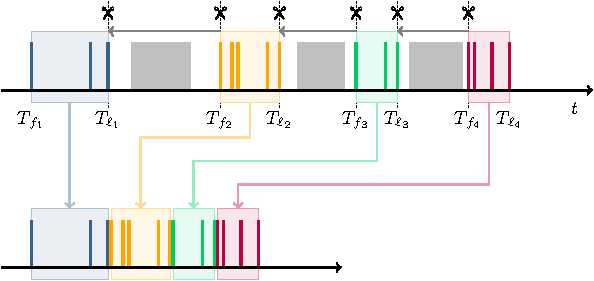
\includegraphics[width=10cm]{images/KSomit.pdf}
  \caption{\label{KSomit} With \texttt{plot.type = "omit"}, the plot
    of \texttt{gof.date} only considers interevents for couples
    falling in the same non-missing period and concatenates them. The
    time interval $(T_{\ell_k},\,T_{f_{k+1}})$ between the last event
    $T_{\ell_k}$ of the non-missing period $k$ and the first event
    $T_{f_{k+1}}$ of the following non-missing period is "cut
    out". The two events $T_{\ell_k}$ and $T_{f_{k+1}}$ collapse into
    \textit{one} event of the new Point Process. Note that a
    non-missing period with less than two events is cut out since it
    contains no valid interevent.  }
\end{figure}

\section{Aggregated (counts) data}
%%------------------------------------------
\label{CountData}

\subsection{Counts}

The \verb@barplotRenouv@ function draws a barplot for counts data and
performs a few tests adapted to this context where events are unknown,
or when interevents can no longer be used.  The data used are $n$ counts $N_i$
for $i=1$, $2$, $\dots$, $n$. These counts must be on \textit{disjoint
  intervals} or "blocks" 
\index{blocks}%
with the \textit{same duration}, e.g.  one year. If events occur
according to an HPP the $N_i$ form a sample of a Poisson
distribution. The barplot compares the empirical (or observed)
frequencies to their theoretical counterparts i.e. the
expectations. The theoretical distribution is estimated using the
sample mean as Poisson parameter (Poisson mean).

The \verb@Brest.years@ object contains aggregated data for one-year blocks. 
Some blocks are incomplete and are listed in \verb@Brest.years.missing@
which can be used in \verb@barplotRenvouv@
\begin{Schunk}
\begin{Sinput}
> data(Brest.years); data(Brest.years.missing)
> bp40 <- barplotRenouv(data = Brest.years, threshold = 40,
             na.block = Brest.years.missing, main = "threshold = 40 cm")
\end{Sinput}
\end{Schunk}
produces the graphic at the left of figure~\ref{BPS}. Increasing the threshold
\begin{Schunk}
\begin{Sinput}
> bp50 <- barplotRenouv(data = Brest.years, threshold = 50,
             na.block = Brest.years.missing, main = "threshold = 50 cm")
\end{Sinput}
\end{Schunk}
we get a barplot for the smaller sample at the right of
figure~\ref{BPS}.  Note that the function guesses that the first
column represents a block indication which may not be true with other
data. Therefore the normal use would specify the \verb@blockname@ and
\verb@varname@ formal arguments of~\verb@barplotRenouv@.

\begin{figure}
  \centering
  \begin{tabular}{c c} 
     \includegraphics[width=8cm]{Rgraphics/fig-bp40.pdf} &
     \includegraphics[width=8cm]{Rgraphics/fig-bp50.pdf} 
\end{tabular}
\caption{\label{BPS}The two barplots produced with
  \texttt{barplotRenouv}. A bar height represents a number of blocks
  (here years) with the number of events given in abscissa.}
\end{figure}

Great care is needed when the data contain missing periods since the 
number of events is then biased downward.

\subsection{Goodness-of -fit}
%%-----------------------------
\index{goodness-of-fit|(}
A popular test for Poisson counts is called \textit{overdispersion test}.
\index{overdispersion index, test}
It is based on the fact that expectation and variance are equal in 
a Poisson distribution. The test statistic is
$$
    I = (n-1)\,S^2/\bar{N}
$$
where $\bar{N}$ and $S^2$ are the sample mean and variance.  Under the
null hypothesis $I$ is approximately distributed as $\chi^2(n-1)$. The
statistic~$I$ tends to take large values when the observations~$N_i$
come from an overdispersed distribution such as the negative
binomial. A one-sided test can therefore be used for a negative
binomial alternative.

A Chi-square Goodness-of-fit 
\index{chi-square goodness-of-fit test}%
test is also available to check the goodness-of-fit of the $N_k$ to a
Poisson distribution. In this test, the counts values $N_k$ are
summarized in a tabular format retaining $m$~distinct values or group
of adjacent values, together with the corresponding frequencies. The
test statistic is
$$
   D^2 = \sum_{k=1}^m \left({O_k-E_k}\right)^2/E_k 
$$
where $O_k$ and $E_k$ are the observed and expected frequencies for
the class $k$. For instance, the first class $k=1$ can be~$N=0$
meaning that $O_1$ and $E_1$ are the number of intervals with no
events recorded. Asymptotically (for large $n$)
$$
   D^2 \sim \chi^2(m-p-1)
$$
where $p$ is the number of parameters estimated from data, here $p=1$
(for the mean of~$N$).  A one-sided test will reject the Poisson
hypothesis when $D^2$ is too large\footnote{That is:
  $D^2>\chi^2_\alpha$}.

A classical drawback
of this test is that classes with a small expected count~$E_i$ 
should be grouped, in order to reach a minimal total of (say) $5$.
\begin{Schunk}
\begin{Sinput}
> bp40$tests
\end{Sinput}
\begin{Soutput}
     statistic  df      p.value
disp  181.4726 113 4.652672e-05
chi2   21.5105   5 6.485040e-04
\end{Soutput}
\begin{Sinput}
> bp50$tests
\end{Sinput}
\begin{Soutput}
      statistic  df   p.value
disp 131.022727 113 0.1181542
chi2   5.722912   3 0.1258975
\end{Soutput}
\end{Schunk}

\noindent
For the dataset \verb@Brest.years@, using a threshold of $50$~cm leads to
acceptable tests (at the $10\%$ level), while $40$~cm seems too small. 
For the chi-square test, more details (e.g. grouping) are available. 

\begin{Schunk}
\begin{Sinput}
> bp50$freq
\end{Sinput}
\begin{Soutput}
  obs.      theo. group
0   31 24.3452997     1
1   27 37.5857258     2
2   31 29.0135427     3
3   18 14.9309460     4
4    4  5.7628213     5
5    1  1.7793974     5
6    2  0.4578567     5
7    0  0.1244104     5
\end{Soutput}
\end{Schunk}

\noindent
The values of $N$ have been grouped in odrer to reach a minimal expected
number of~$5$ for each group.

Note that for a fairly high threshold, the statistic~$N$ will
generally take only the two values $0$ and $1$. Then the chi-square
test which requires at least three classes will not be available.
\index{goodness-of-fit|)}
\chapter{\texttt{Renouv} objects}
%%=================================

\label{Chap-Renouv}
  
Fitted POT models are in \pkg{Renext} considered as objects of a
\verb@"Renouv"@ S3 class, and can be used with methods \verb@coef@,
\verb@vcov@, \verb@plot@, \verb@predict@, $\dots$ Such models are
usually created by a ML estimation using the creator function
\verb@Renouv@. This function can carry out the usual estimation from
observations $X_i$ of the marked process. It can also cope with
heterogeneous data including blocks such as \verb@MAXdata@ or
\verb@OTSdata@ described in previous chapters, e.g. to use historical
information. In some rare cases, a \verb@Renouv@ object can also be
created with \verb@RenouvNoEst@ if all coefficients are known.

\index{Renouv class@{\texttt{Renouv} class}|(}

%%\section{First example: high tide surge heights at Brest}
%%================================================================
  
\section{Fitting POT for La Garonne}
%%========================================
\label{FitGaronne}
\index{Garonne data@{\texttt{Garonne} data}|(}
For the dataset \verb@Garonne@, the OT data contain flow values over
the threshold $u_\star = 2500~\textrm{m}^3/\textrm{s}$. We can fit a POT
model with any threshold $u \geqslant 2500$. As in~\citet{MIQUELBOOK}
we fit an exponential and a two-parameter Weibull distribution using
OT data only.  The \verb@Renouv@ function needs on input the \textit{levels}
given in a vector \verb@x@, the \textit{effective duration} \verb@effDuration@
--~normally in years~-- and the \textit{threshold}

\index{exponential distribution}
\begin{Schunk}
\begin{Sinput}
> fit.exp <- Renouv(x = Garonne$OTdata$Flow, effDuration = 65, threshold = 3000,
                    distname.y = "exponential", main = "exponential")
\end{Sinput}
\begin{Soutput}
Special inference for the exponential case without history
\end{Soutput}
\begin{Sinput}
> class(fit.exp)
\end{Sinput}
\begin{Soutput}
[1] "Renouv"
\end{Soutput}
\end{Schunk}

\noindent
The result is an object with (S3) class \verb@"Renouv"@. A few S3 
methods are available for this class:

\begin{Schunk}
\begin{Sinput}
> methods(class = "Renouv")
\end{Sinput}
\begin{Soutput}
 [1] AIC     anova   BIC     coef    lines   logLik  nobs    plot    PPplot 
[10] predict print   QQplot  summary vcov   
see '?methods' for accessing help and source code
\end{Soutput}
\end{Schunk}

\noindent
The method \verb@coef@ extracts the vector of estimated coefficients
\begin{Schunk}
\begin{Sinput}
> coef(fit.exp)
\end{Sinput}
\begin{Soutput}
      lambda         rate 
1.5076923077 0.0009695003 
\end{Soutput}
\end{Schunk}

\noindent
The first element named \verb@"lambda"@
is the event rate expressed in \textit{events by year}. The other elements are the ML
estimates of the distribution for excesses, with names
corresponding to the probability functions --~here one name
\verb@"rate"@ for the exponential distribution parameter.
The ubiquitous
\verb@plot@ method can be used to re-draw a return level plot 
from the fitted object. The \verb@summary@ method can be used to display the results.
The \verb@predict@ method can be used to compute
return levels corresponding to given return periods as illustrated later.
\index{return level!in POT}
\index{predict method@{\texttt{predict} method}}


A \verb@Renouv@ object is mainly a list within which the
\verb@estimate@ element gives the maximum likelihood estimates
returned by \verb@coef@. Many other results are returned.

\begin{Schunk}
\begin{Sinput}
> head(names(fit.exp), n = 24)
\end{Sinput}
\begin{Soutput}
 [1] "call"        "x.OT"        "y.OT"        "nb.OT"       "effDuration"
 [6] "threshold"   "distname.y"  "p.y"         "parnames.y"  "fixed.y"    
[11] "trans.y"     "est.N"       "cov.N"       "est.y"       "cov.y"      
[16] "corr.y"      "estimate"    "fixed"       "df"          "nobs"       
[21] "p"           "opt"         "logLik"      "logLikFun"  
\end{Soutput}
\end{Schunk}

\noindent
This shows the $24$ first elements in the list. The \verb@sigma@ element gives the
vector of standard deviations for the estimates.

The \verb@distname.y@ formal in \verb@Renouv@ 
is used to change the distribution for the excesses~$Y_i=X_i-u$.
\begin{Schunk}
\begin{Sinput}
> fit.weibull <- Renouv(x = Garonne$OTdata$Flow, effDuration = 65, threshold = 3000,
                        distname.y = "weibull", main = "Weibull")
> coef(fit.weibull)
\end{Sinput}
\begin{Soutput}
     lambda       shape       scale 
   1.507692    1.063710 1057.298215 
\end{Soutput}
\begin{Sinput}
> fit.weibull$sigma
\end{Sinput}
\begin{Soutput}
      lambda        shape        scale 
  0.15229992   0.08451114 106.04186243 
\end{Soutput}
\end{Schunk}
\index{Weibull distribution}

\noindent
The estimated parameters of the Weibull distribution and their
\index{Weibull distribution} standard deviation (list item
\verb@sigma@) show that the shape is close to~$1.0$, which corresponds
to the exponential distribution. The two fits produced return level
plots shown on figure~\ref{RLP1}.


\begin{figure}
   \centering
   \begin{tabular}{c c} 
     \includegraphics[width=8cm]{Rgraphics/fig-feGaronne.pdf} &
     \includegraphics[width=8cm]{Rgraphics/fig-fwGaronne.pdf} 
   \end{tabular}
   \caption{\label{RLP1}Return level plots for the example 
     \texttt{Garonne} with two distributions
     for the excesses.}
\end{figure}


\section{Return level plot}
%%============================
\subsection{Description} 
%%----------------------
\index{return level!plot|(} 
\index{Gumbel plot}% 
\textbf{Renext} uses a
return level plot which may be qualified as \textit{exponential}, and
differs from the usual one which uses \textit{Gumbel} scales.  The
main difference is that the exponential plot uses a log scale for
return periods while the Gumbel plot uses a log-log scale.  In both
cases, the theoretical return level curve (exponential/Gumbel) shows
as a straight line.

The difference between the two plots is restricted to the small
levels/return periods, since the exponential and Gumbel distribution
functions are close for large values.  As it was advocated in the
discussion about functional plots page~\pageref{FUNCPLOTS}, the
exponential return level plot is better suited to the use of "OTdata"
i.e. data where only values over a threshold are kept, even if
the the original observations $X_i$ are Gumbel see~\ref{GEVGPD}.

The return level plot is similar to the classical exponential plot of
the previous chapter, \index{exponential plot}%
\textit{but with the two axes $x$, $y$ exchanged}. A concave
(downward) RL plot indicates a distribution with a tail "lighter than
the exponential" or even with finite end-point such as GPD with
$\xi<0$.

The displayed confidence limits are in all cases pointwise and
bilateral, and correspond to the confidence percents displayed which
can be changed in the call. In most cases the confidence limits are
approximate and obtained by using the \textit{delta method} briefly 
described later. 
\index{delta method}%
For some special cases with exponential distribution an exact
inference is possible and used. The \verb@infer.method@ element in the
list returned by \verb@Renouv@ provides information about this.

\subsection{Plot method for \texttt{Renouv} objects} 
%%-----------------------------------------------
\label{plot.Renouv}
Once created with the \verb@Renouv@ function, an object of class
\verb@"Renouv"@ can be used to (re)draw a return level plot and change
some options. Useful changes concern the main title using the
\verb@main@ argument, or axes labels \verb@xlab@, \verb@ylab@.  Axis
limits can also be set.  For the return levels, this is done using the
usual \verb@ylim@ argument.  For the return periods, the limits are
set using \verb@Tlim@ or \verb@problim@.  The first possibility works
with a vector containing two return periods (in years); the second
possibility requires a vector with two probabilities.

\index{axes limits in return level plot}

The two following code chunks produce the return level plots shown on
figure~\ref{RLP2}.  On left panel, we change the return periods axis
limits.

\begin{Schunk}
\begin{Sinput}
> plot(fit.weibull,  Tlim = c(1, 100), main = "return periods from 0 to 100 years")
\end{Sinput}
\end{Schunk}

\noindent
On the right panel we change both axes and the confidence level.

\begin{Schunk}
\begin{Sinput}
> plot(fit.weibull, Tlim = c(1, 100), ylim = c(3000, 10000), pct.conf = 95,
       main = "return levels and 95% limits")
\end{Sinput}
\end{Schunk}

\index{confidence limits!level choice}
\noindent
The chosen percentage for the confidence limits \verb@pct.conf = 95@
must correspond to a value available in the object description.
Otherwise, it is necessary to force a new prediction by passing a
suitable \verb@pct.conf@ argument along with \verb@predict = TRUE@ in
the call to the \verb@plot@ method.  The shown elements of the
\verb@Renouv@ object can be selected, see
chapter~\ref{Chap-RenextGraphics} p.~\pageref{Chap-RenextGraphics} for
more details.

\begin{figure}
   \centering
   \begin{tabular}{c c} 
     \includegraphics[width=8cm]{Rgraphics/fig-rlGaronneOpt1.pdf} &
     \includegraphics[width=8cm]{Rgraphics/fig-rlGaronneOpt2.pdf} 
   \end{tabular}
   \caption{\label{RLP2}Changing the settings of the return level plot. 
     Left and right: the limits of the $x$-axis are set using \texttt{Ylim}. 
     Right: \texttt{ylim} and \texttt{pdc.conf} are used and only the 
     specified $0.95$ confidence level is shown.}
\end{figure}

\index{plotting positions|(} 

When only OT data are used as here, the default plotting positions use
a return period at the order statistics $Z_1 > Z_2 > \dots > Z_n$ estimated by $1 /
\widehat{T}(Z_i) = \widehat{\lambda} \,\widetilde{S}(Z_i)$, where
$\widehat{\lambda}$ is the natural estimate of the rate (see below)
and $\widetilde{S}(Z_i) = 1 - \widetilde{F}(Z_i) = i / (n +1)$. 
Alternatively, the \verb@ppoints@ formula~(\ref{eq:CUNNAME}) for $a \neq 0$ or Nelson's 
formula \citep{Nelson} can be specified with \verb@plotOptions@ passed
to the \verb@SandT@ function. The difference between the different choices
can be important for the largest order statistics (i.e. for small $i$).

\index{return level!plot|)}
\index{plotting positions|)} 

%% Most are transformations of one another so that choice is partly
%% a matter of taste.


\section{Computational details}
%%==================================
\subsection{Maximum Likelihood theory}
%%--------------------------------
\index{maximum likelihood|(} 
Estimation and inference in \textbf{Renext} mainly
rely on the Maximum Likelihood (ML) theory. A relevant presentation can be found
in \citet[chap.~2]{COLES} or in the \textit{Further reading}
references given there.

The standard application context of ML is when an ordinary sample i.e. 
$n$ independent random variables $X_i$ with the same distribution depending 
of an unknown vector $\bs{\theta}_X$ with density $f_X(x;\bs{\theta}_X)$. 
The likelihood function~$L$ is the joint density of the sample i.e.
$$
   L = \prod_{i=1}^n f_X(X_i;\,\bs{\theta}_X)
$$
and the estimator $\widehat{\bs{\theta}}_X$ is the value of~$\bs{\theta}_X$ 
maximising~$L$.
In some special cases the maximisation of~$L$ can have an explicit solution,
but a numerical optimisation will generally be required. The ML theory
warrants\footnote{Under suitable \textit{regularity conditions}.} the
\textit{asymptotic unbiasedness} and \textit{asymptotic normality}: 
when $n$ is large $\widehat{\bs{\theta}}_X$ has its expectation approximately 
equal to the true unknown $\bs{\theta}_X$, and it is approximately normally distributed.    

The ML theory applies to more general situations where observations are
no longer independent or can have different marginal distributions. This 
occurs when order statistics are used in the estimation, e.g. with 
historical data.
\index{historical data}%

The general principle of the \verb@Renouv@ function is to allow a large choice
of distributions, yet trying to take advantage of the specific distribution/independence 
when possible. In most cases the maximisation of the likelihood is obtained using 
\verb@optim@ function of the \verb@stats@ package. When historical data are used
they are considered as a complement to the ordinary data (excesses) 
and two optimisations might be used. 
\index{optim function@{\texttt{optim} function}}
\index{maximum likelihood|)}

\subsection{Estimation and inference}
%%--------------------------------
The model uses a parameter vector $\bs{\theta} =
[\lambda,\,\bs{\theta}_X^\top ]^\top$ of length~$p$ formed with the
HPP rate~$\lambda$ and the parameter vector $\bs{\theta}_X$ for the
levels distribution.

\textit{When only OT data are used}, the observed data consist in $N$ events 
$[T_i,\,X_i]$ on a given period. Since events $T_i$
and levels~$X_i$ are independent the likelihood is
$$
   L_{\texttt{OT}} = 
   \underset{\mathrm{events}}{\underbrace{\frac{(\lambda w)^N}{N!} e^{-\lambda w}}}
   \times 
   \underset{\mathrm{levels}}{\underbrace{\prod_{i=1}^N f_X(X_i;\,\bs{\theta}_X)}}
$$
where $w$ is the time-length (i.e. the effective duration), and the log-likelihood is
\begin{equation}
  \label{eq:LLstand}
  \log L_{\texttt{OT}}  = N\log(\lambda w) - \lambda w 
    - \log(N!)+ \sum_{i=1}^N \log f_X(X_i;\,\bs{\theta}_X). 
\end{equation}
The ML estimation consists in two simple ML estimations: one for the events 
(rate estimation) and the other for levels. The ML estimate of the unknown rate $\lambda$ is
$$
     \widehat{\lambda} = \frac{N}{w}= \frac{\textrm{number of events}}{\textrm{duration}},
$$
its variance is $\Var[\widehat{\lambda}]= \lambda/w \approx
\widehat{\lambda}/w$.  Note that the number of events $N$ is a
\textit{sufficient statistic} for $\lambda$: the events $T_i$ are not
used and the whole information they provide about~$\lambda$ is
contained in~$N$.  The "$X$-part" of ML concerns an ordinary
sample. The ML estimate $\widehat{\bs{\theta}}_X$ is available in
closed form in some cases (e.g. exponential) or can be computed by
using a specific method (e.g.  GPD, Weibull, gamma), see
\citet{RenCompDet}.

\textit{When only OT data are used}, it can be said that $\lambda$ and
$\bs{\theta}_X$ are orthogonal parameters.  This is no longer true
when block data (e.g. historical data) are also used: the likelihood
then takes a slightly more complex form given below.
\index{orthogonal parameters}

In a few cases with only OT data and favourable distribution
(e.g. Weibull), it is possible to use the \textit{expected}
information matrix. But the general treatment in \textbf{Renext} is
based on the \textit{observed} information and the numerical
derivatives. More precisely, the information matrix is obtained as the
\index{hessian}%
\index{information matrix!observed}%
numerical hessian at convergence. The hessian can either be the
element \verb@hessian@ returned by the \verb@optim@ function, or
result from the use of the \verb@hessian@ function from
the \verb@numDeriv@ package: see the manual for more details.


\subsection{Delta method}
%%--------------------------
\index{inference!delta method}
The \textit{delta method}
\index{delta method}% 
can be used to infer about a  function\footnote{Smooth enough.}
$\psi = \psi(\bs{\theta})$ of the parameter $\bs{\theta}$. For instance 
$\psi(\bs{\theta})$ can be the return period of a given level~$x$
%%, which depends on $\lambda$ and $\bs{\theta}_X$
(see~\ref{eq:RETPER}).  The transformed parameter estimate is
$\widehat{\psi} = \psi(\widehat{\bs{\theta}})$.  As a general result
in the ML framework, the transformed parameter estimate is
asymptotically unbiased $ \Esp[\widehat{\psi}] \approx
\psi(\bs{\theta}) $ and asymptotically normal with variance
$$
     \Var[\widehat{\psi}] \approx 
     \bs{\delta}^\top \,\Var[\widehat{\bs{\theta}}]\,\bs{\delta}     
$$
where $\bs{\delta}$ is the gradient vector 
$$
  \bs{\delta} = \frac{\partial \psi}{\partial \bs{\theta}} =  
  \left[\frac{\partial \psi}{\partial \theta_1}, \,
        \frac{\partial \psi}{\partial \theta_2}, \, \dots, \, 
      \frac{\partial \psi}{\partial \theta_p}\right]^\top
$$
evaluated at $\widehat{\bs{\theta}}$, see~\citet[chap. 2]{COLES}. 

\pkg{Renext} uses this approach\footnote{In the \texttt{predict} method for 
\texttt{Renouv} objects.}
with $\psi$ taken as the level (or
quantile)~$x(T)$ corresponding to a given return period~$T$, given by
(\ref{eq:RETLEV}) in section~\ref{RETPERLEV}. Using chain rule, the
derivative with respect to the rate $\lambda$ is
\begin{equation*}
  \frac{\partial}{\partial \lambda} x(T) = \frac{1}{\lambda^2 T f_X}
\end{equation*}
where the density $f_X$ is evaluated at $x(T)$. In practice, the
uncertainty on $\lambda$ has a minor impact for large return periods
and can optionally be ignored in the computations. The
gradient of the quantile function with respect to $\bs{\theta}_X$ is
computed numerically using a finite difference approximation.


\subsection{Goodness-of-fit}
%%------------------------
\index{goodness-of-fit|(}
As a general tool to assess the fit, the Kolmogorov-Smirnov (KS) test
is computed in all cases. 

\index{Kolmogorov-Smirnov test}
The KS test normally requires a \textit{completely specified} distribution 
for the null hypothesis while the \textit{fitted} distribution is used here 
--~thus generating a bias. In some special cases (normal, exponential) the bias 
could be corrected using an adaptation depending on the distribution as in
Lilliefors test for the normal. However since the number of estimated parameters 
is small (usually $1$ or $2$ for the "excesses part") the bias will be small 
provided that the number of exceedances is large enough, say $50$ or more. 

For some distributions such as exponential a specific test may be
available.  In the current version distribution-specific tests are in
\verb@Renouv@ limited to Bartlett's test of exponentiality.

Rounded measurements often lead to ties in the sample, which
\index{ties} \index{jitter} 
would without precaution generate a warning in the KS test.
This can be avoided by "jitterising" i.e. adding a small random noise
to the observed values.

The  graphical analysis of the fit using the return level plot is generally 
instructive. For  exponential or Weibull excesses, classical exponential or
Weibull plot can also be drawn using the~\verb@expplot@ and~\verb@weibplot@ functions. 
\index{Weibull plot}%
\index{exponential plot}

When block data (e.g. historical data) are given, they are used during
the estimation but not included in the empirical distribution in the
KS test. In this case, the interpretation of the test needs further
investigations.  \index{goodness-of-fit|)}

% On an exponential plot
% $$
%    - \log \left[1 - F(y) \right] 
% $$


\section{Using heterogeneous data}
%%---------------------------------
\label{SECHISTORY}
\index{heterogeneous data|(}
\index{historical data|(}
\index{block data|(}

\subsection{Two types of block data}
%%-----------------------------------------
\label{TwoTypes}
Beside OT data, \verb@Renouv@ and other \pkg{Renext} functions can use
two other sorts of data: MAX data which are $r$ largest, and OTS data
for ``Over Threshold Supplementary'' data\footnote{Or Over
  ThresholdS.}.  In both cases, the data are structured in blocks and
can be used only as complement to the main OT data.
%% which must continue to be provided.

\begin{description}
  
\item[MAX data] contain $r$~largest blocks. Each block corresponds to
  a time interval of known duration $w$ during which the $r$ largest
  values are available. Blocks are assumed to be mutually disjoint and
  disjoint from the OT period. Neither the duration of blocks nor the
  number $r$ of observations are assumed to be constant; hence each
  block~$b$ has a specified duration $w_b$ and a number $r_b$ of
  largest values.

%%so the  
%%observations random vectors for blocks and over the OT period
%%are mutually independent.

\item [OTS data] contain Over Threshold blocks with known duration, 
  exceedances and levels (or excesses). Again, blocks are assumed to be mutually
  disjoint and disjoint from the OT period and other 
  blocks. For each such block $b$ with known duration $w_b$, we must
  have a threshold $u_b$ and all observations with levels exceeding
  $u_b$. The number $r_b$ of such observations may be zero, in which
  case we may say that $u_b$ is an \textit{unobserved level}. The
  threshold~$u_b$ can not be smaller than the main threshold.

  \index{threshold!perception}

\end{description}
\index{unobserved level}

In the context of historical information, the threshold $u_b$ of an
OTS block can be called a \textit{perception} threshold.  Unobserved
levels (empty OTS blocks) occur when it is granted, or at least
believed, that $u_b$ was never exceeded during a period of time. For
instance it can be granted that a river never flooded over a given
benchmark level during the last five centuries, or that the arch of a
bridge was never reached since its construction. Such information has
obviously a great potential impact on the estimation since it
typically concerns very long periods, much longer than the observation
period. Note that the unobserved level can concern missing periods for
OT data: although no data are available we may still know that no very
high level occurred, see figure~\ref{UNOBSERVED}.
  
\begin{figure}
  \centering
  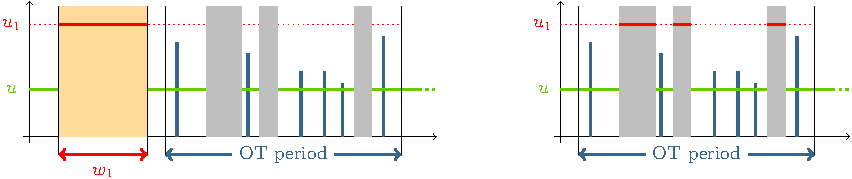
\includegraphics[width=14cm]{images/unobserved.pdf}
  \caption{\label{UNOBSERVED} An unobserved level can provide
    information on an historical period (left) or on missing periods
    (right). In the second case, one would use a virtual block with
    its duration $w_1$ set to the sum of all gaps lengths.}
\end{figure}


\subsection{Likelihood}
%%--------------------

\subsubsection{Global likelihood}
%% ------------------
In the general setting of heterogeneous data described above, the log-likelihood
takes the form
$$
\log L = \log L_{\texttt{OT}} + \log L_{\texttt{MAX}} + \log L_{\texttt{OTS}}, 
$$
because the OT period and MAX or OTS blocks are assumed to correspond
to disjoint time intervals and hence to independent observations. Similarly
the log-likelihood for MAX or OTS data are sums of contributions arising from independent 
blocks, so
$$
\log L =  \log L_{\texttt{OT}} + 
\sum_{b \in \{\texttt{MAX blocks}\} } \log L_b + \sum_{b \in \{\texttt{OTS blocks}\}} 
\log L_b.
$$ 
The log-likelihood for a MAX or OTS block is given below.

\subsubsection{MAX data}
%%------------------
\index{MAXdata@{\texttt{MAXdata}}|(}%
Consider a MAX block $b$ with duration $w_{b}$. 
Let $Z_{b,1} \geqslant Z_{b,2} \geqslant \dots \geqslant Z_{b,r_b}$ 
be the~$r_b$ largest observations. The log-likelihood for the block can be proved to be 
\index{rlargest@{$r$~largest}}
\begin{equation}
  \label{eq:LLH1}
  \log L_b  = r_b  \log(\lambda w_{b}) + \sum_{i=1}^{r_b} \log f_X(Z_{b,i};\,\bs{\theta}_X)  
  -\lambda w_{b} \, S_X(Z_{b,r};\,\bs{\theta}_X)
\end{equation}
up to an unimportant additive constant.

%% When several blocks exist, they provide independent random vectors 
%% of observations with possibly different~$r_b$ and the log-likelihood
%% is obtained by summing over blocks.
\index{MAXdata@{\texttt{MAXdata}}|)}%

\subsubsection{OTS data}
%%------------------
\label{LOTSdata}
\index{OTSdata@{\texttt{OTSdata}}|(}%
The likelihood for an OTS block with threshold $u_{b}$ is simpler
to derive. According to the POT assumptions\footnote{See section~\ref{ASSUMPTIONS}
page~\pageref{ASSUMPTIONS}.}, 
the levels greater than $u_{b}$ occur
according to an HPP \textit{thinning} the 
original HPP%
\index{thinning (Poisson Process)}. 
This thinned process has rate $\lambda S_X(u_{b})$ because at
each OT event, the level~$u_{b}$ can be exceeded with
probability~$S_X(u_{b})$. Let $w_{b}$ be as before the block duration,
and let $Z_{b,1} \geqslant Z_{b,2} \geqslant \dots \geqslant
Z_{b,r_b}$ be the~$r_b$ observations, with possibly $r_b=0$. Up to an
additive constant, the log-likelihood is
\begin{equation}
  \label{eq:LLH_OTS}
  \log L_b  = r_b  \log(\lambda w_{b}) 
    + \sum_{i=1}^{r_b} \log f_X(Z_{b,i};\,\bs{\theta}_X)  
  -\lambda w_{b} \,S_X(u_{b};\,\bs{\theta}_X).
\end{equation}
This expression is identical to~(\ref{eq:LLH1}) with the block
threshold $u_{b}$ replacing the minimum observed value~$Z_{b,r_b}$.

When an OTS block~$b$ contains no observation i.e. when $r_b=0$,
the log-likelihood~(\ref{eq:LLH_OTS}) is simply
\begin{equation}
  \label{eq:LLH2}
     \log L_b =  - \lambda w_{b} \, S_X(u_{b};\,\bs{\theta}_X).
\end{equation}
This is easily checked: on a period of length $w_{b}$, the
number of levels $>u_{b}$ is Poisson with mean $\mu :=
S_X(u_{b}) \times \lambda w_{b}$.  Hence the probability to observe no
level~$>u_{b}$ is: $ e^{-\mu} \mu^0/0!= e^{-\mu}$.  

\index{OTSdata@{\texttt{OTSdata}}|)}%


\subsubsection{Remarks}
%%------------------
Assume that we have OT data, and consider the impact of using
one extra block. Some special cases arise.

\begin{enumerate}
\item When only one OTS block with no observation and with
  $u_{b}$ equal to the main threshold, its contribution to the global
  log-likelihood is $-\lambda w_{b}$ since then $S_X(u_{b})=1$
  in~\ref{eq:LLH2}).  Up to an unimportant constant, the resulting
  global log-likelihood is identical to the one which would result from
  simply adding~$w_{b}$ to the effective duration $w$ of the main OT sample
  in (\ref{eq:LLstand}).
  
\item Assume that we have only one historical MAX block which only
  contains the maximum $Z_{b,1}$ i.e. has $r_b=1$.  The contribution
  of the block to the log-likelihood~(\ref{eq:LLH1}) is
  $$
  \log L_b = \log(\lambda w_{b}) + \log f_X(Z_{b,1};\,\bs{\theta}_X)
  -\lambda w_{b} \, S_X(Z_{b,1};\,\bs{\theta}_X).
  $$
  At the right hand side, the third term is identical to~(\ref{eq:LLH2})
  with an unobserved level $u_{b}=Z_{b,1}$ and a period length
  $w_{b}$. The sum of the two first terms at right hand side is the extra
  contribution that would be added to the log-likelihood of the OT data
  if a new OT observation with level~$Z_{b,1}$ had been added without
  changing the main OT period duration. Therefore, the same
  likelihood/results are obtained in the two following approaches.
  \begin{list}{$\bullet$}{ \setlength{\itemsep}{2pt}
      \setlength{\topsep}{2pt} }
  \item Specify an historical MAX block of length $w_{b}$ with $r_b=1$
    and level $Z_{b,1}$.
  \item Join the observed maximum~$Z_{b,1}$ to the OT levels $X_i$, and
    specify that the level $u_{b}:=Z_{b,1}$ was never reached during a
    OTS block of length $w_{b}$.
  
  \end{list}
  The second approach might seem natural to practitioners.
  
\end{enumerate}

\subsubsection*{Likelihood maximisation}
%%------------------
\index{constraint!inequality in MLE}
\index{optim function@{\texttt{optim} function}}
When heterogeneous data are used, the ML estimators of $\lambda$ and
~$\bs{\theta}_X$ are found by numerically maximising the log-likelihood.
It can be shown that this likelihood function can be concentrated with
respect to the rate $\lambda$, thus 
\index{concentration, likelihood}
leading to the maximisation of a function $\log
L_{\textrm{c}}(\bs{\theta}_X)$ depending on~$\bs{\theta}_X$ only,
see~\citet{RenCompDet}. 

The numerical maximisation relies on the~\verb@optim@ function. Like
most EV packages do, \pkg{Renext} uses an unconstrained optimisation,
while most distributions would normally require the use of inequality
constraints. For instance with GPD excesses, constraints should be
imposed because the maximal likelihood is otherwise infinite,
see~\ref{GPDdist}. In practice, this is not really a concern because
the log-likelihood will take the value \verb@NA@ or \verb@NaN@ rather
than a large value near the boundary of the parameter domain, and
\verb@optim@ copes quite well with a \verb@NA@ value of the objective.

By default, the initial values for the estimation with heterogeneous
data are obtained as the ML estimates based on the OT data only. The
reason is that MAX or OTS data were regarded as complementary
data in the initial conception of \pkg{Renext}. Moreover, the ML
estimation based on OT data is simplified for most of the
distributions used in practice.


\index{initial values}


\subsection{Example: using Garonne historical MAX data}
%%-------------------------------------  
As seen in chapter~\ref{Chap-Intro}, the \verb@Garonne@ dataset
contains historical data of type MAX, which can be used in the
estimation. The data are described in the section~\ref{HistoricalData}
page~\pageref{HistoricalData}.  The historical part corresponds here
to one block, and the following levels

\begin{Schunk}
\begin{Sinput}
> Garonne$MAXdata$Flow
\end{Sinput}
\begin{Soutput}
 [1] 7500 7400 7000 7000 7000 6600 6500 6500 6400 6300 6300 6200
\end{Soutput}
\end{Schunk}

\noindent
The duration is given in \verb@Garonne$MAXinfo$duration@
with value 143.09~years.

As a general rule, the MAX or OTS data must in \verb@Renouv@ be passed
as a \textit{list} of numeric vectors, each vector corresponding to
one block. The (effective) durations are given as a numeric vector
with the \textit{same length as the list}. For the MAX case, the
formal arguments to use are \verb@MAX.data@ (list) and
\verb@MAX.effDuration@ (numeric vector).

Since the data corresponds here to one block, the list \verb@MAX.data@
contains only one vector and the vector \verb@MAX.effDuration@
is of length one. The two following fits produce the return level plots shown 
in figure~\ref{FIGHIST}.

\begin{Schunk}
\begin{Sinput}
> fit.exp.H <- Renouv(x = Garonne$OTdata$Flow,
                      effDuration = 65, threshold = 3000,
                      MAX.data = list(Garonne$MAXdata$Flow),
                      MAX.effDuration = Garonne$MAXinfo$duration,
                      distname.y = "exponential",
                      main = "Garonne data, \"exponential\" with MAXdata")
\end{Sinput}
\end{Schunk}

\begin{Schunk}
\begin{Sinput}
> fit.weib.H <- Renouv(x = Garonne$OTdata$Flow,
                       effDuration = 65, threshold = 3000,
                       MAX.data = list(Garonne$MAXdata$Flow),
                       MAX.effDuration = Garonne$MAXinfo$duration,
                       distname.y = "weibull",
                       main = "Garonne data, \"Weibull\" with MAXdata")
\end{Sinput}
\end{Schunk}

\noindent
The exponential fit is only slightly modified by the use of historical data. 
As said before, the parameter $\lambda$ and $\bs{\theta}_X$ are no longer
orthogonal when historical data are used

\begin{Schunk}
\begin{Sinput}
> fit.exp.H$corr
\end{Sinput}
\begin{Soutput}
          lambda      rate
lambda 1.0000000 0.2054784
rate   0.2054784 1.0000000
\end{Soutput}
\end{Schunk}


\begin{figure}
   \centering
   \begin{tabular}{c c} 
     \includegraphics[width=8cm]{Rgraphics/fig-feGaronneH.pdf} &
     \includegraphics[width=8cm]{Rgraphics/fig-fwGaronneH.pdf} 
   \end{tabular}
   \caption{
     \label{FIGHIST}
     Return level plots for the example \texttt{Garonne} with two
     distributions for the excesses and historical data. Specific
     plotting positions are used to take into account the historical
     observations. The twp plots can be compared to those of
     figure~\ref{RLP1}.}
\end{figure}

\subsection{Plotting positions}
%%-----------------------------
\label{MAXPLOTPOS}
\index{plotting positions|(}
\index{censoring|(}
To be displayed on the return level plot (see figure~\ref{FIGHIST}),
MAX or OTS data require suitable plotting positions. Naive
plotting positions based on predictions where used in former
versions of \pkg{Renext}. They are now replaced by more elaborated
ones arising from some relevant literature on censored data~\citep{EnvStat}. 
The principle is most easily understood for OTS data. 
\begin{itemize}
\item If there is only one OTS block with threshold $u_1>u$ and
  duration $w_1$, then we can easily estimate the return period of the
  level $u_1$ by counting the total number of exceedances over $u_1$
  (including those during the OT period). The product $\lambda
  S_X(u_1) = 1/T(u_1)$ is estimated as the number of exceedances
  divided by the duration $w + w_1$. The plotting positions for the 
  observations above $u_1$ are determined as usual, see 
  section~\ref{plot.Renouv} above, with the estimated rate $\widehat{\lambda}$ 
  replaced by $1 / \widehat{T}(u_1)$.  The number of
  exceedances over $u$ is then estimated by assuming that the
  observations with levels in $(u, \,u_1)$ occurred in the $w_b$ 
  years of the block with the known rate for the $w$ years of the
  OT data. We thus can estimate the return period $T(u)$ 
  of $u$ and then those of the observations with level
  between $u$ and $u_1$ using an interpolation.

\item When $B$ OTS blocks exist, the threshold $u$ and the $B$
  thresholds $u_b$ can without loss of generality be assumed to be
  ordered as $u_{0} < u_{1} < \dots < u_{B}$ with $u_{0} := u$, and
  thus define $B +1$ slices of levels $(u_{b},\,u_{b+1})$ for $0
  \leqslant b \leqslant B$ with $u_{B+1} := \infty$. The previous
  computation still applies for the upper slice which correspond to
  levels in $>u_{B}$.  Starting from this highest slice, one can
  then estimate by recursion the number of observations falling in
  each of the slices $(u_{b},\,u_{b+1})$ for $b=B$, $B-1$, $\dots$,
  $0$, and thus the return periods $T(u_{b})$.  The computation is
  similar to that described by~\citet{HirschStedinger} for the
  survival. The plotting positions for the observations in a slice
  result from an interpolation.
\end{itemize}


For MAX blocks, the plotting positions are computed by considering a
MAX block as an OTS block with it its threshold set near to the
smallest observation in the block, i.e. $u_b:= Z_{b,r_b} - \epsilon$
in the notations used in~(\ref{eq:LLH1}) where $\epsilon$ is
small. The chosen value of $\epsilon$ depends on the data.

For instance, for the data \verb@Garonne@ with $B=1$, the MAX block
can be considered as an OTS block with threshold 
$u_1 = 6200-\epsilon = 6195~\textrm{m}^3/\textrm{s}$.  The total number of
observations in the upper slide $(u_1, \,\infty)$ is $3 + 12 = 15$
(in the OT sample and the MAX block), during 
$w + w_1 = 65 + 143.09 = 208.09$~years. 
So the return period of $u_1$ is
$208.09/15 = 13.9$~years.
Now the number of observations in the next slide 
$(u_0,\,u_1)$ is estimated by using the rate of such observations
during the OT period.

The computations are carried out by the \verb@SandT@ function which estimates both the
survival $S$ and the return periods $T$. Details are provided in
\cite{RenCompDet}.

\index{plotting positions|)}
\index{censoring|)}

\index{historical data|)}
\index{heterogeneous data|)}
\index{block data|)}

\subsection{Fitting from Rendata objects}
%%----------------------------------------
\index{Rendata class@{\texttt{Rendata} class}|(} 

Recall that a S3 class \verb@"Rendata"@ is defined in \textbf{Renext}
in order to represent heterogeneous data with optional block or historical
data. An object of class \verb@"Rendata"@ contains an OT sample, but
also embeds useful pieces of information such as the effective
duration for the OT sample or the variable name.  It seems sensible to
use these indications in a POT model by simultaneously passing them as
formal arguments to the fitting function.  For instance, when the OT
sample of a \verb@"Rendata"@ object is used in a fit, the effective
duration could consistently be taken from this object.  \verb@Renouv@
can indeed be used by giving an \verb@x@ formal with class
\verb@"Rendata"@ instead of a numeric vector.

\begin{Schunk}
\begin{Sinput}
> fitWithObj <- Renouv(x = Garonne)
\end{Sinput}
\end{Schunk}

\noindent
Note that the threshold is taken from the \verb@Rendata@ object's \verb@OTdata@ part, and
will generally be too small for a POT modelling. It can be changed
simply

\begin{Schunk}
\begin{Sinput}
> fitWithObj1 <- Renouv(x = Garonne, threshold = 3000)
\end{Sinput}
\end{Schunk}

\noindent
Similarly, the effective duration of the object can
be shortcut by providing the \verb@effDuration@ formal argument 
in the call. The distribution of the excesses can be set in the usual way.
In all cases, the \verb@summary@ method should be invoked on the fitted 
object.

Using \verb@"Rendata"@ objects passed as \verb@x@ formals can simplify the task 
of fitting many datasets files if these are read with the \verb@readXML@ function.
\index{readXML function@{\texttt{readXML} function}}
\index{Rendata class@{\texttt{Rendata} class}|)}

\section{GPD excesses}
%%===============================

\subsection{Standard POT}
%%----------------------------
Of course, the \verb@Renouv@ function can be used with a GPD for the excesses.

\begin{Schunk}
\begin{Sinput}
> fit.GPD <- Renouv(x = Garonne$OTdata$Flow, effDuration = Garonne$OTinfo$effDuration, 
                    threshold = 3000, distname.y = "GPD",
                    main = "Garonne data, \"GPD\"")
> coef(fit.GPD)
\end{Sinput}
\begin{Soutput}
      lambda        scale        shape 
   1.5076923 1160.1536041   -0.1226653 
\end{Soutput}
\end{Schunk}

\noindent
The fitted distribution has a negative shape 
$\widehat{\xi} = -0.12$, hence
has a finite upper end-point, which makes a major difference with the 
Weibull fit. The maximal level is thus estimated
as $u - \widehat{\sigma}/\widehat{\xi} =   
12458$. 

As before, we can use the historical information in \verb@Garonne@

\begin{Schunk}
\begin{Sinput}
> fit.GPD.H <- Renouv(Garonne, threshold = 3000, distname.y = "GPD",
                      main = "Garonne data, \"GPD\" with MAXdata")
> coef(fit.GPD.H)
\end{Sinput}
\begin{Soutput}
      lambda        scale        shape 
   1.5547065 1321.6227580   -0.1853906 
\end{Soutput}
\end{Schunk}
The maximal level is now estimated
as  $10129$. 

\begin{figure}
   \centering
   \begin{tabular}{c c} 
     \includegraphics[width=8cm]{Rgraphics/fig-fGPDGaronne.pdf} &
     \includegraphics[width=8cm]{Rgraphics/fig-fGPDGaronneH.pdf} 
   \end{tabular}
   \caption{
     \label{FIGGPD} Using GPD excesses for \texttt{Garonne}.
   }
\end{figure}

\subsection{Several parameterisations}
%%-------------------
\index{Lomax distribution|(}
\index{maxlo distribution|(}
The Lomax and maxlo\footnote{We use this new name for
  an important yet apparently unnamed distribution. While 
  the Lomax distribution is named after K.S. Lomax, no
  Mrs or Mr Maxlo seems famous yet for having used it, hence the name does not require
  a capital letter.
}
distributions are re-parameterisations of the GPD with shape $\xi > 0$ and
$\xi <0$ respectively, see~\ref{LOMAX} and \ref{MAXLO}. In both cases,
the distribution involves a scale parameter $\beta>0$ and a shape
parameter $\alpha>0$. The exponential corresponds to a limit when $\alpha
\to \infty$ and $\beta \to \infty$ while $\beta / \alpha$ tends to a
finite limit $\sigma>0$.

\begin{Schunk}
\begin{Sinput}
> fit.maxlo <- Renouv(x = Garonne$OTdata$Flow,
                      effDuration = Garonne$OTinfo$effDuration, 
                      threshold = 3000, distname.y = "maxlo")
> coef(fit.maxlo)
\end{Sinput}
\begin{Soutput}
     lambda       shape       scale 
   1.507692    8.152266 9457.880896 
\end{Soutput}
\end{Schunk}

\noindent
The scale parameter of the maxlo distribution is upper end-point for the excess, hence
the upper end-point for the level is estimated as 
$u + \widehat{\beta} = 12458$ as it was with the \verb@GPD@ distribution.

Choosing the Lomax distribution would here give an error

\begin{Schunk}
\begin{Sinput}
> trylomax <- try(Renouv(x = Garonne$OTdata$Flow,
                         effDuration = Garonne$OTinfo$effDuration,
                         threshold = 3000, distname.y = "lomax"))
> class(trylomax)
\end{Sinput}
\begin{Soutput}
[1] "try-error"
\end{Soutput}
\begin{Sinput}
> cat(trylomax)
\end{Sinput}
\begin{Soutput}
Error in flomax(x = y, info.observed = info.observed) : 
  CV < 1. Estimation impossible for "lomax"
\end{Soutput}
\end{Schunk}

\index{coefficient of variation} 
\noindent
When only OT data are used in the
estimation, only one of the two distributions Lomax and maxlo can be
fitted with \verb@Renouv@ without producing an error. Indeed, a
finite ML estimator exists for the Lomax distribution if and only if the empirical
coefficient of variation $\widehat{\mathrm{CV}}$ is greater
than~$1$, while a finite ML estimator exists for the maxlo
if and only~$\widehat{\mathrm{CV}} < 1$. Note that for a
sample of size $n$ of a GPD with $\xi >0$ small, the probability that
$\widehat{\mathrm{CV}} < 1$ hence that the ML estimation of the Lomax
is impossible is not always negligible. For $\xi = 0$ the probability
that $\widehat{\mathrm{CV}} < 1$ is computed by the \verb@pGreenwood1@
function.

Again, when MAX or OTS data are used only one of the two distributions
Lomax and maxlo can be fitted

\begin{Schunk}
\begin{Sinput}
> fit.maxlo.H <- Renouv(Garonne, threshold = 3000, distname.y = "maxlo")
> coef(fit.maxlo.H)
\end{Sinput}
\begin{Soutput}
     lambda       shape       scale 
   1.554721    5.391524 7126.255255 
\end{Soutput}
\end{Schunk}

\noindent
The situation can be quite confusing  when MAX or OTS data are
used because it is possible then that the sign of the ML estimator of
the GPD shape~$\xi$ differs depending on whether the block data (MAX
and OTS) are used or not.  In such a case, it is simpler to directly use
\verb@GPD@.

\index{predict method@{\texttt{predict} method}}
The return levels for the GPD or its re-parameterisation as Lomax or
maxlo are identical. Inasmuch the delta method is used, the confidence
intervals on the RL are identical as well, up to small 
numerical differences.

\begin{Schunk}
\begin{Sinput}
> predict(fit.GPD, newdata = c(100, 200))
\end{Sinput}
\begin{Soutput}
    period    quant     L.95    U.95     L.70     U.70
100    100 7345.885 6018.570 8673.20 6643.998 8047.772
200    200 7762.568 6073.465 9451.67 6869.367 8655.769
\end{Soutput}
\begin{Sinput}
> predict(fit.maxlo, newdata = c(100, 200))
\end{Sinput}
\begin{Soutput}
    period    quant     L.95     U.95     L.70     U.70
100    100 7345.885 6018.570 8673.200 6643.998 8047.772
200    200 7762.568 6073.466 9451.669 6869.367 8655.768
\end{Soutput}
\end{Schunk}

\index{Lomax distribution|)}
\index{maxlo distribution|)}


\section{Fixing parameter values}
%%======================================

\index{fixed parameter values|(}

\subsection{Problem}
%%---------------
In some situations one may want to fix one or several parameters in the
distribution of excesses and still perform a ML estimation for
the remaining parameters. For instance, the \verb@shape@ of a Weibull 
distribution can be fixed while the \verb@scale@ is to be estimated.
%% This can be viewed as a radical bayesian scheme with the fixed parameters
%% receiving an 'ultra-informative' Dirac prior.  

The \verb@Renouv@ function supports fixed parameters, with some limitations. 
In the current version, the HPP rate parameter \textit{$\lambda$ can not
be fixed}, and \textit{at least one parameter must be estimated
in the excesses part}. Thus the full model must have at least two
non-fixed parameters.

The specification of the fixed parameter is done using the 
\verb@fixed.par.y@ formal argument in \verb@Renouv@. Its value
must be a named vector list with names in the distribution parnames.
As a general rule\footnote{In some special cases, this is unnecessary
but harmless.}, 
the non-fixed (estimated) parameters must
be given using the \verb@start.par.y@ arg with a similar
list value.
\index{initial values}

\subsection{Example}
%%--------------------
The fixed parameter option can work with or without 
historical data in the same manner.

\begin{Schunk}
\begin{Sinput}
> fit.weib.fixed.H <- 
    Renouv(x = Garonne$OTdata$Flow,
           effDuration = 65, threshold = 3000,
           MAX.data = list(Garonne$MAXdata$Flow),
           MAX.effDuration = Garonne$MAXinfo$duration,
           distname.y = "weibull",
           fixed.par.y = c(shape = 1.4),
           start.par.y = c(scale = 2000),
           trace = 0,
           main = "Garonne data, \"Weibull\" with MAXdata and fixed shape")
\end{Sinput}
\end{Schunk}
\begin{Schunk}
\begin{Sinput}
> fit.weib.fixed.H$estimate
\end{Sinput}
\begin{Soutput}
     lambda       shape       scale 
   1.579748    1.400000 1326.602872 
\end{Soutput}
\end{Schunk}

\noindent
With some distributions such as the SLTW some parameters \textit{must}
be fixed.  Here the shift parameter \verb@delta@ is fixed 
to~$\delta =2800~\textrm{m}^3/\textrm{s}$ meaning that we 
believe that excesses over~$u-\delta=500$ are Weibull, 
even if we only know excesses over the 
threshold~$u=3000~\textrm{m}^3/\textrm{s}$.
\index{SLTW distribution}

\begin{Schunk}
\begin{Sinput}
> fit.SLTW.H <- 
    Renouv(x = Garonne$OTdata$Flow,
           effDuration = 65, threshold = 3000,
           MAX.data = list(Garonne$MAXdata$Flow),
           MAX.effDuration = Garonne$MAXinfo$duration,
           distname.y = "SLTW",
           fixed.par.y = c(delta = 2800, shape = 1.4),
           start.par.y = c(scale = 2000),
           main = "Garonne data, \"SLTW\" with MAXdata, delta and shape fixed")
\end{Sinput}
\end{Schunk}

\noindent
When some parameters are fixed the covariance contains structural
zeros, and consequently the correlation matrix contains non-finite coefficients.

\begin{Schunk}
\begin{Sinput}
> fit.SLTW.H$cov
\end{Sinput}
\begin{Soutput}
            lambda delta shape       scale
lambda  0.02270571     0     0   -2.950236
delta   0.00000000     0     0    0.000000
shape   0.00000000     0     0    0.000000
scale  -2.95023609     0     0 9881.428891
\end{Soutput}
\end{Schunk}

\begin{figure}
   \centering
   \begin{tabular}{c c} 
     \includegraphics[width=8cm]{Rgraphics/fig-fixweibGaronneH.pdf} &
     \includegraphics[width=8cm]{Rgraphics/fig-fixSLTWGaronneH.pdf} 
   \end{tabular}
   \caption{Return level plots for the example \texttt{Garonne} with two distributions 
     with \textbf{fixed parameters} (and historical data).}
\end{figure}

\subsection{All parameters known}
%%--------------------------------------
\index{RenouvNoEst@{\texttt{RenouvNoEst}}}
Using \verb@Renouv@ with its \verb@fixed.par@ argument is possible  when
some of the parameters are known, but not all of them.
The \verb@RenouvNoEst@ function can be used to create a \verb@Renouv@
object with all its parameters known, including the Poisson 
rate~$\lambda$. This can be useful to use \verb@plot@ or \verb@predict@
with known parameters. See the help \verb@?RenouvNoEst@ for 
an example.

\index{fixed parameter values|)}


\section{Likelihood Ratio tests}
%%=======================================
\index{Likelihood Ratio test|(}

\subsection{Using the \texttt{anova} method}
%%----------------------
In section~\ref{FitGaronne}, two POT models were fitted using the same
\verb@Garonne@ data with exponential and Weibull distributions for the
excesses. The ML estimate for the Weibull shape was $\widehat{\alpha} =
1.06$, and since the
exponential distribution corresponds to Weibull with shape $\alpha =
1$, it seems natural to test the hypothesis $H_0:\,\alpha=1$ against
the alternative $H_1:\,\alpha \neq 1$.

\index{constraint!equality (test of)} 
More generally, we can consider
two \textit{nested models}: the null hypothesis $H_0$ imposes some
restrictions\footnote{Equality constraints.}  on the parameter
vector~$\bs{\theta}$ which is unrestricted under the alternative
$H_1$. The Likelihood Ratio (LR) statistic is obtained by maximising
the restricted and unrestricted likelihoods as 
\index{nested models}%
$$
\textrm{LR} :=
%%\frac{L(\widehat{\bs{\theta}}_0)}{L(\widehat{\bs{\theta}}_1)} =
\frac{\textrm{maximal likelihood under }H_0}{\textrm{maximal
    likelihood under }H_1},
$$
with values $\textrm{LR} \leqslant 1$. It is often convenient to use
the test statistic $W := - 2 \log \textrm{LR}$, which takes values
$W\geqslant 0$ and is the difference of the \textit{deviances} $D :=
-2 \log L$.  \index{deviance} A large value for $W$ tells that
$H_0$ should be rejected.  Under some general conditions, it
can be proved that $W$ has asymptotic distribution $\chi^2(r)$ where
$r$ is the number of independent scalar restrictions imposed by the
null hypothesis, so $r=1$ in the exponential vs Weibull case.

LR tests are often made available in R packages through the
\verb@anova@ method which must be implemented for the class of fitted
models that we wish to test. The \verb@anova@ methods compare nested
models fitted \textit{with the same data}.  In a general context, it
is enough to extract the log-likelihood and the number of parameters
for each model. The  statistic $W$ above is computed and compared to its
asymptotic distribution.  In \pkg{Renext}, the \verb@anova@ method was
implemented for the \verb@Renouv@ class. For instance using two
\verb@Renouv@ objects created before 
\begin{Schunk}
\begin{Sinput}
> anova(fit.exp, fit.weibull)
\end{Sinput}
\begin{Soutput}
Models: 
  o 'fit.exp' with exceedances dist. "exponential"
  o 'fit.weibull' with exceedances dist. "weibull"

Method used:  asymptotic approximation 

Analysis of Deviance Table

            df deviance       W Pr(>W)
fit.exp      2   1556.0               
fit.weibull  3   1555.4 0.58725 0.4435
\end{Soutput}
\end{Schunk}

\index{Weibull distribution}%

\noindent
which tells that the null hypothesis of an exponential distribution
must here be rejected at any level $\alpha \leqslant
0.44$ and
accepted for larger values of $\alpha$. So in practice we would here
accept~$H_0$.

Note that the same test statistic $W$ could have been used to test
$H_0$ against the thin-tailed Weibull alternative $H_1: \alpha >1$,
which seems in better accordance with the data. But the asymptotic
distribution of $W$ would then no longer be $\chi^2$, and be that of
the product $BC$ of two independent random variables with Bernoulli
and chi-square distributions $B \sim \texttt{Ber}(1/2)$ and $C \sim
\chi^2(1)$.
%% \citep{Kozubowski}. 
The reason is that the tested value of the parameter is now on the
boundary of parameter domain, and the statistic $W$ takes the value
$0$ when $\widehat{\alpha}<1$.  For $w >0$ we have $\Pr\{BC > w\} =
\Pr\{ B=1 \} \Pr\{ C > w \}$, so the $p$-value for $H_1: \alpha <1$ is
about 
$0.22$ 
and the exponentiality would thus still be rejected.

%% <<>>=
%% pchisq(4.02, df = 1, lower.tail = FALSE) 
%% @ 

\subsection{LR test for the GPD family}
%%----------------------
\index{Lomax distribution|(}
\index{maxlo distribution|(}
\index{exponential distribution|(}
In the standard POT framework, excesses are assumed to follow a GPD, say
$\texttt{GPD}(0,\,\sigma,\,\xi)$. Depending on the sign of $\xi$, very
different tail behaviour and return levels will be obtained.  Not
infrequently, the ML estimate $\widehat{\xi}$ is close to zero 
thus suggesting to test the null hypothesis~$\xi = 0$ corresponding to
the exponential distribution.  Three (composite) alternative
hypotheses are often of interest
$$
   \textrm{H}_0: \: \xi = 0 \: (\textrm{exponential}) \quad 
   \textrm{against} \qquad  \textrm{H}_1:
   \begin{cases} 
     \xi \neq 0 & \textrm{(GPD)},\\
     \xi > 0    & \textrm{(Lomax)},\\
     \xi < 0    & \textrm{(maxlo)}.\\
   \end{cases}
$$  
The LR still can be used as test statistic. However, a well-known
problem is that the distribution of the LR ratio has a \textit{very
  slow convergence} to its asymptotic distribution in the present
context\footnote{See e.g. \cite{Kozubowski}}.  More than $100$ excesses
are typically needed to obtain a $p$-value with a two-digit
precision. For instance, with the Lomax alternative, the probability
to obtain $W=0$ under $H_0$ is the probability that
$\widehat{\mathrm{CV}}<1$ and is given by the \verb@pGreenwood1@
function related to the Greenwood's statistic. For $n=50$, we get
$\Pr\{W = 0\} \approx 0.6$
while the asymptotic probability mass is $0.5$.  
\index{Greenwood's statistic}

To overcome this problem of slow convergence, the distribution of the
test statistic for a given sample size $n$ has been computed by
Monte-Carlo simulations and a statistical model was fitted to allow a
more precise evaluation of the distribution of~$W$
\citep{RenCompDet}. This approximation is used in the
\verb@LRexp.test@ and also in the \verb@anova@ method for the
\verb@Renouv@ class as far as no MAX or OTS data are used.

\begin{Schunk}
\begin{Sinput}
> anova(fit.exp, fit.GPD)
\end{Sinput}
\begin{Soutput}
Models: 
  o 'fit.exp' with exceedances dist. "exponential"
  o 'fit.GPD' with exceedances dist. "GPD"

Method used:  numerical approximation 

Analysis of Deviance Table

        df deviance       W Pr(>W)
fit.exp  2     1556               
fit.GPD  3     1555 0.99712 0.3444
\end{Soutput}
\begin{Sinput}
> anova(fit.exp, fit.maxlo)
\end{Sinput}
\begin{Soutput}
Models: 
  o 'fit.exp' with exceedances dist. "exponential"
  o 'fit.maxlo' with exceedances dist. "maxlo"

Method used:  numerical approximation 

Analysis of Deviance Table

          df deviance       W Pr(>W)
fit.exp    2     1556               
fit.maxlo  3     1555 0.99712 0.2343
\end{Soutput}
\end{Schunk}

\noindent
So none of the two tests would reject exponentiality.

The LR test also works with heterogeneous data. However the usual
asymptotic approximation will still be used as soon as the compared
fits used MAX or OTS block data. 

\begin{Schunk}
\begin{Sinput}
> anova(fit.exp.H, fit.GPD.H)
\end{Sinput}
\begin{Soutput}
Models: 
  o 'fit.exp.H' with exceedances dist. "exponential"
  o 'fit.GPD.H' with exceedances dist. "GPD"

Method used:  asymptotic approximation 

Analysis of Deviance Table

          df deviance      W Pr(>W)
fit.exp.H  2   1714.2              
fit.GPD.H  3   1710.0 4.1515  0.318
\end{Soutput}
\begin{Sinput}
> anova(fit.exp.H, fit.maxlo.H)
\end{Sinput}
\begin{Soutput}
Models: 
  o 'fit.exp.H' with exceedances dist. "exponential"
  o 'fit.maxlo.H' with exceedances dist. "maxlo"

Method used:  asymptotic approximation 

Analysis of Deviance Table

            df deviance      W Pr(>W)
fit.exp.H    2   1714.2              
fit.maxlo.H  3   1710.0 4.1515  0.159
\end{Soutput}
\end{Schunk}

\noindent 
So when the historical data are used, the exponentiality hypothesis
is still accepted against the $\xi < 0$ alternative, but the 
$p$-value is now smaller. 

%% As a rule of thumb, the asymptotic approximation is acceptable when
%% the whole information used in the fit is equivalent to $120$ standard
%% POT observations.

Concerning the specific application to the \verb@Garonne@ data, it
must be said that the tests give pretty different results when the
threshold varies in the range $[2500, \,3500]$. For instance,
the exponentiality is rejected at the $5\%$ level when the 
threshold is taken as $3200$.
\index{maxlo distribution|)}

\subsection{Other tests for  the exponential-GPD context}
%%-------------------------------------
As far as only OT data are used, two other tests of \pkg{Renext} can
be used to test the exponential $\xi = 0$ against the Lomax
alternative. These tests use the squared coefficient of variation
%% ${\widehat{\mathrm{CV}}^2}$ 
and the Jackson's statistic and named
\textit{$\mathrm{CV}^2$ test} 
(or \textit{WE test}, for Wilk's Exponentiality test) and
\textit{Jackson's test}. As for the LR test, the distribution of the test
statistic for both of these tests is approximated thanks to a
statistical model fitted on simulated values.  In accordance with the
results of \citet{Kozubowski}, the Jackson's test was found on
simulations to be nearly as poweful as the LR test, both having
greater power than the $\mathrm{CV}^2$ test.

We can use these two tests for the excesses of the \verb@Garonne@
example, although the Lomax alternative $H_1: \xi > 0$ is clearly
not well supported by the data

\begin{Schunk}
\begin{Sinput}
> X <- Garonne$OTdata$Flow
> Y <- X[X > 3000]
> c(CV2 = CV2.test(Y)$p.value, Jackson = Jackson.test(Y)$p.value)
\end{Sinput}
\begin{Soutput}
    CV2 Jackson 
      1       1 
\end{Soutput}
\begin{Sinput}
> Y <- X[X > 3300]
> c(CV2 = CV2.test(Y)$p.value, Jackson = Jackson.test(Y)$p.value)
\end{Sinput}
\begin{Soutput}
    CV2 Jackson 
  0.581   1.000 
\end{Soutput}
\end{Schunk}

\noindent
So both tests accept $H_0: \xi = 0$ against the Lomax alternative.
The computed $p$-value in these tests can be $1$ (exactly), which may
seem unusual.  The reason is that the $p$-value is computed with a
precision which is not greater than two digits and is rounded.  This
is not a concern for large $p$-values ($\approx 1$).

\index{Garonne data@{\texttt{Garonne} data}|)}
\index{Lomax distribution|)}
\index{test of exponentiality!likelihood ratio}
\index{test of exponentiality!Jackson's}
\index{test of exponentiality!WE or Wilk's or $\mathrm{CV}^2$}

\index{Greenwood's statistic}
\index{Jackson's test}

\index{Likelihood Ratio test|)}
\index{exponential distribution|)}

\index{Renouv class@{\texttt{Renouv} class}|)}

\chapter{POT and block data}

\label{Chap-POTBlocks}

Although devoted to POT, \pkg{Renext} can be used for some analyses
involving block data: block maxima and $r$ largest. These
possibilities are restricted to models arising form the marked process
with a distribution of levels in the GPD family, including
exponential, Lomax or maxlo distributions.

\section{Example: Venice data}
%%===================
\index{rlargest@{$r$~largest}|(}
\index{block maxima|(}
\index{venice data@{\texttt{venice} data}|(}

Consider the \textit{Venice} data, concerning the sea-level at Venice (in cm).
This dataset is used as example~1.5 in Coles' book, where it used
in section~3.5.3 for a $r$~largest analysis. Variants
of this dataset are provided by several CRAN 
packages\footnote{E.g. with a \texttt{Year} column in \textbf{ismev}.}. We will
use here the \textit{data frame} object named \verb@venice@ from \pkg{evd}.
\index{evd package@{\textbf{evd} package}}
\begin{Schunk}
\begin{Sinput}
> head(venice, n = 3)
\end{Sinput}
\begin{Soutput}
       1   2   3   4   5  6  7  8  9 10
1931 103  99  98  96  94 89 86 85 84 79
1932  78  78  74  73  73 72 71 70 70 69
1933 121 113 106 105 102 89 89 88 86 85
\end{Soutput}
\begin{Sinput}
> range(venice, na.rm = TRUE)
\end{Sinput}
\begin{Soutput}
[1]  69 194
\end{Soutput}
\end{Schunk}

\noindent
We have $51$ years of data from
$1931$ to
$1981$ and for each year the $r$
largest observations for $r \leqslant 10$, given in descending
order. Missing observations are present in year 1935, and then given
as \verb@NA@.

We may regard the observations as arising from a POT model, and
hence use them as MAX data blocks, all with duration equal to one
year.  For that aim, we need to build a list with one element by year:
a numeric vector with the $r$~largest values observed that year,
e.g. $r=5$.

\begin{Schunk}
\begin{Sinput}
> r <- 5
> MAX.data <- as.list(as.data.frame(t(venice[ , 1:r])))
> MAX.data <- lapply(MAX.data, function(x) x[!is.na(x)])
> MAX.effDuration <- rep(1, length(MAX.data))
> head(MAX.data, n = 2)
\end{Sinput}
\begin{Soutput}
$`1931`
[1] 103  99  98  96  94

$`1932`
[1] 78 78 74 73 73
\end{Soutput}
\begin{Sinput}
> head(unlist(lapply(MAX.data, length)))
\end{Sinput}
\begin{Soutput}
1931 1932 1933 1934 1935 1936 
   5    5    5    5    5    5 
\end{Soutput}
\end{Schunk}

\noindent
Note that the transposition method \verb@t@ returns a \textit{matrix},
and a coercion to \verb@data.frame@ is required to get a list.


Since all observations are $>66$~cm, we can consider a POT model with
$u \leqslant 66$ to use all available information. Then we can the use the
\verb@Renouv@ function

\begin{Schunk}
\begin{Sinput}
> fit.GPD <- Renouv(x = NULL, 
                    MAX.data = MAX.data, MAX.effDuration = MAX.effDuration,
                    distname.y = "GPD", threshold = 66,
                    numDeriv = FALSE, trace = 0, plot = FALSE)
> coef(fit.GPD)
\end{Sinput}
\begin{Soutput}
     lambda       scale       shape 
27.51085268 18.28501439 -0.08798975 
\end{Soutput}
\end{Schunk}

\noindent
We implicitly supposed that for each year the $r$ provided observations
are the largest, even when \verb@NA@ are found.
Since the fitted object has class \verb@"Renouv"@, the \verb@plot@
method shows the usual RL plot

\begin{Schunk}
\begin{Sinput}
> plot(fit.GPD)
\end{Sinput}
\end{Schunk}

\noindent
see fig.~\ref{VenicerLarg}. The plotting positions for the points are
obtained as explained in section~\ref{MAXPLOTPOS}.

\begin{figure}
  \centering
  \begin{tabular}{c} 
     \includegraphics[width=7cm]{Rgraphics/fig-venice5.pdf} 
   \end{tabular}
   \caption{\label{VenicerLarg} 
     Fit using $r$~largest values from the \texttt{venice} data
     set.  The plotting positions are obtained as explained in
     section~\ref{MAXPLOTPOS}.}
\end{figure}

For \verb@Renouv@ objects using a distribution in the GPD family, a
``translation'' of the parameters to GEV parameters for block maxima is
provided in the \verb@MAX@ element of the result.

\begin{Schunk}
\begin{Sinput}
> fit.GPD$MAX
\end{Sinput}
\begin{Soutput}
$distname
[1] "gev"

$blockDuration
[1] 1

$estimate
         loc        scale        shape 
118.56917923  13.65946564  -0.08798975 

$sigma
       loc      scale      shape 
1.56641520 0.77521523 0.03292705 

$cov
               loc      scale        shape
loc    2.453656585 0.74275331 -0.005386851
scale  0.742753305 0.60095866  0.012692692
shape -0.005386851 0.01269269  0.001084191
\end{Soutput}
\end{Schunk}

\noindent
The translation provides the estimated parameters of a GEV
distribution $\texttt{GEV}(\mu^\star,\sigma^\star,\,\xi^\star)$ and
must not be confused with those of the $\texttt{GPD}(u,\sigma,\,\xi)$
for the excesses of the POT model. The estimated values of the shape
parameters $\xi$ and $\xi^\star$ are the always the same, but the
estimated scale parameters differ and $\mu^\star$ is not equal to the
threshold $u$.  The GEV distribution can be used as usual in the
$r$~largest context. If a different threshold had been used, e.g. $u =
50$ the POT parameters would have been very different, but the GEV
parameters would have been the same.

%% Note however that for the
%% POT model with event rate $\lambda$, a block of duration $w$ can be
%% empty hence have no maxima: this occurs with the probability
%% $e^{-\lambda w}$. 



\section{Using \texttt{fGEV.MAX}}
%%===========================================
\index{GEV distribution!ML estimation|(}
Beside \verb@Renouv@, the \verb@fGEV.MAX@ function was added to
\pkg{Renext} to perform the estimation of a GEV distribution
$\texttt{GEV}(\mu^\star,\,\sigma^\star, \xi^\star)$ from block maxima
or from $r$~largest observations, using in both cases blocks having
\textit{the same duration}.  This function uses the representation of
the GEV as the distribution of the block maxima in a POT model with
GPD excesses. The distribution is no longer a formal argument, and nor
is the threshold $u$ which is chosen depending on the data. In the
likelihood~$L$, the POT rate $\lambda$ has been concentrated out, so $L$
depends only on the two parameters $\sigma$ and $\xi$ of the POT
model. Although computation time is not really a concern here, the
optimisation is much faster than the usual one which uses the three
GEV parameters $\mu^\star$ $\sigma^\star$ and $\xi^\star$.  The
hessian at the optimum is computed using analytical derivatives rather
than numerical derivatives. Details can be found in \cite{RenCompDet}.


\begin{Schunk}
\begin{Sinput}
> fit.GEV <- fGEV.MAX(MAX.data = MAX.data, MAX.effDuration = MAX.effDuration)
> fit.GEV$estimate
\end{Sinput}
\begin{Soutput}
         loc        scale        shape 
118.57054271  13.66158562  -0.08789015 
\end{Soutput}
\begin{Sinput}
> require(ismev)
> fit.GEVref <- rlarg.fit(venice, show = FALSE)
> fit.GEVref$mle
\end{Sinput}
\begin{Soutput}
[1] 120.5479027  12.7840265  -0.1129418
\end{Soutput}
\end{Schunk}

\noindent
Note that \verb@fGEV.MAX@ returns a simple \verb@list@ object and the
methods such as \verb@coef@ can not be used.

\index{GEV distribution!ML estimation|)}

\index{block maxima|)}
\index{rlargest@{$r$~largest}|)}
\index{venice data@{\texttt{venice} data}|)}

\section{Computing the $r$ largest observations}
%%========================================
\label{OT2MAX}
\index{OT2MAX function@{\texttt{OT2MAX} function}|(}
\index{missing periods!in blocks|(}

\subsection{Coping with gaps}
%%-----------
Given observations $[T_i,\,X_i]$ of the marked process, it seems quite
easy to compute block maxima or $r$~largest --~in other words, to
aggregate the data.  However, in some cases gaps are present and must
be taken into account in the aggregation. When known gaps exist in the
data, they should be carefully inspected to assess their possible 
impact on the estimation. 

The \verb@OT2MAX@ function was designed to compute the $r$~largest
observations as well as some diagnostics when known missing periods
exist. The formal argument \verb@OTdata@ of this function corresponds
to a data frame with two columns: a \verb@date@ column and a column
containing the variable~$X$, as in the \verb@OTdata@ element of an
object of the \verb@"Rendata"@ class. The \verb@maxMissingFrac@ gives
the maximum fraction (between $0$ and $1$) of gap within a block. When
this fraction is exceeded in a block, the returned block observations are
\verb@NA@.  By default, the function produces a plot as shown in figure~\ref{DUNKMAX}. 

The \verb@Dunkerque@ data set used here is similar to \verb@Brest@:
it also concern sea surge and embeds missing periods, but the data
cover a smaller period of time.

\index{Dunkerque data@{\texttt{Dunkerque} data}}

\begin{Schunk}
\begin{Sinput}
> RD <- Dunkerque
> OTdata <- RD$OTdata; OTmissing <- RD$OTmissing
> ## allow up to 50% of gap within each block, or only 5%?
> MAX1 <- OT2MAX(OTdata = OTdata, OTmissing = OTmissing,
                 maxMissingFrac = 0.5,
                 main = "impact of the 'maxMissingFrac' formal")
> MAX2 <- OT2MAX(OTdata = OTdata, OTmissing = OTmissing, dataFrames = TRUE,
                 prefix = "Max", maxMissingFrac = 0.05, plot = FALSE)
> lines(MAX2$MAXdata$date, MAX2$MAXdata$Surge, type = "h", col = "red", lwd = 3)
> legend("topleft", lw = c(1, 3), col = c("black", "orangered"),
         legend = c("50% max", " 5% max"))
\end{Sinput}
\end{Schunk}

\noindent
The \verb@OTmissing@ element of \verb@Dunkerque@ reports quite large
gaps in the nineties (e.g. from October of 1992 to July of 1995).  With the
larger value \verb@maxMissingFrac = 0.5@, up to $50\%$ of a block can
be a gap, and fewer \verb@NA@ block observations result than when
a small value of \verb@maxMissingFrac@ is used.



\begin{figure}
\begin{tabular}{c c} 
     \includegraphics[width=7cm]{Rgraphics/fig-Dunk1.pdf} & 
     \includegraphics[width=7cm]{Rgraphics/fig-Dunk2.pdf} 
   \end{tabular}
   \caption{\label{DUNKMAX} Left: block maxima for \texttt{Dunkerque}
   with \texttt{maxMissing} set to \texttt{0.5} and
   \texttt{0.05}. Right: the $r$ largest observations 
   for $r=4$. Each annual block can contain up to $4$ 
   observations.
 }
\end{figure}

\begin{Schunk}
\begin{Sinput}
> ## r largest obs for r = 4
> MAX3 <- OT2MAX(OTdata, OTmissing = OTmissing, MAX.r = 4,
                 maxMissingFrac = 0.9, 
                 dataFrames = FALSE, trace = TRUE,
                 main = "r largest with r = 4")
\end{Sinput}
\begin{Soutput}
Number of events by block 
1956 1957 1958 1959 1960 1961 1962 1963 1964 1965 1966 1967 1968 1969 1970 1971 
   2    7   11   13   12   13   11   15    6    9   18   22   29   18   17   11 
1972 1973 1974 1975 1976 1977 1978 1979 1980 1981 1982 1983 1984 1985 1986 1987 
  13   16    9   14   11   15   10   17   14   29   29   29   21   17   17   13 
1988 1989 1990 1991 1992 1993 1994 1995 1996 1997 1998 1999 2000 2001 2002 2003 
  17    4    5   NA   NA   NA   NA    1    7    8   14   16   19   28   22   17 
2004 2005 2006 2007 2008 
  24   19   20   31   NA 
\end{Soutput}
\begin{Sinput}
> ## restrict the period
> MAX4 <- OT2MAX(OTdata, OTmissing = OTmissing, MAX.r = 4,
                 start = "1962-01-01",
                 end = "1990-01-01",
                 maxMissingFrac = 0.9, 
                 dataFrames = FALSE, trace = TRUE,
                 main = "r-largest with r = 4 with given 'start' and 'end'")
\end{Sinput}
\begin{Soutput}
Number of events by block 
1962 1963 1964 1965 1966 1967 1968 1969 1970 1971 1972 1973 1974 1975 1976 1977 
  11   15    6    9   18   22   29   18   17   11   13   16    9   14   11   15 
1978 1979 1980 1981 1982 1983 1984 1985 1986 1987 1988 1989 
  10   17   14   29   29   29   21   17   17   13   17    4 
\end{Soutput}
\begin{Sinput}
> ## use in a block maxima analysis, as if there were no gaps.
> fitDunk <- fGEV.MAX(MAX.data = MAX3$data,
                      MAX.effDuration = rep(1, length(MAX3$effDuration)))   
\end{Sinput}
\end{Schunk}

\subsection{Diagnostics for gaps}
%%--------------------------------------
\label{DiagGaps}
A quite common problem with gaps is that they can conceal a seasonal
effect: the probability that a randomly selected time $T$ falls in a
gap can differ according to the season of $T$. Even if the gaps are
really exogenous, this may cause a bias in models, either POT or block
maxima. For example severe storm surges occur mainly in winter, so a
gap with a six month duration will probably lead to loose more of
large observations when it is located in winter rather than in
summer. This can be controlled by estimating the probability that $T$
falls in a gap according to its location in the year. The
\verb@plotType@ argument of \verb@OT2MAX@ provides an useful related
diagnostic.

\begin{Schunk}
\begin{Sinput}
>  ## plot the gap rate
> MAX5 <- OT2MAX(OTdata = OTdata, OTmissing = OTmissing,
                  maxMissingFrac = 0.5,
                  main = "probability of being in a  gap",
                  plotType = "gap")
\end{Sinput}
\end{Schunk}

\noindent
The plot (fig~\ref{DUNKDIAG}, left) shows that the probability of falling
in a gap does not have a very strong variation along one year, and
broadly ranges from $1/5$ to $1/3$. The horizontal segments in gray
show jitterised versions of the gap rates for all the year $\times$
month pairs. Many of these rates are equal to $0$ (no gap in the month) and
several of them are equal to $1$ (fully missing month).

A complementary diagnostic is obtained by plotting a yearly time
series for each month of a year (as in fig~\ref{DUNKDIAG} right), thus
showing the evolution of the gap fraction in a given month.

\begin{Schunk}
\begin{Sinput}
> require(lattice)
> xyplot(MAX5$monthGapTS[ , c(1:3, 10:12)], type = "h", lwd = 2, ylim = c(0, 1))
\end{Sinput}
\end{Schunk}

\noindent
The \pkg{lattice} base package \citep{PACKlattice} used here
provides nice plots for multiple time series.

\begin{figure}
\begin{tabular}{c c} 
     \includegraphics[width=7cm]{Rgraphics/fig-Dunk3.pdf} & 
     \includegraphics[width=7cm]{Rgraphics/fig-Dunk4.pdf} 
   \end{tabular}
   \caption{
     \label{DUNKDIAG}
     Controlling the possible impact of gaps. Left: the probability
     that a day in the year falls in a gap is shown in orange. The
     horizontal segments in gray show a jitterised version of the gap
     fraction for a year/month combination. Right: yearly time series
     of gap fraction for six months.  \index{jitter}}
\end{figure}



\index{OT2MAX function@{\texttt{OT2MAX} function}|)}
\index{missing periods!in blocks|)}
\chapter{Renext graphics}

\label{Chap-RenextGraphics}
\index{return level!plot|(}

%\section{}
%%---------------------------
\pkg{Renext} graphics are based on the \pkg{graphics} package and can
hence be customised as usual. However, adding points to a RL plot is
not always easy: when several types of data exist, the determination
of the plotting positions requires quite technical computations as
performed by the \verb@SandT@ function.

A number of supplementary functions are provided to facilitate the
most frequent modifications of RL plots. A widespread practice is
showing on a same RL plot the data (sample points) and some elements
of a fitted model: quantile line, confidence bounds. When several
kinds or sources of data are used in the fit, it is important to
display them in such a way that the different sources are readily
identified.  It arose from users practice that representing \textit{several}
fits on the same RL plot through a \verb@lines@ or \verb@points@
method is often a valuable option, provided that the fits can be
identified by colour or line type, and that a legend is shown: the
\verb@RLpar@ function and the \verb@RLlegend*@ functions have been
designed for these two tasks.

\section{The \texttt{plot} and \texttt{lines} methods}
%%---------------------------
\index{confidence limits!shown or not}
\index{Garonne data@{\texttt{Garonne} data}|(}
The \verb@plot@ and \verb@lines@ methods can be used to build return level plots
showing several elements: quantile line (or return level line), sample points,
$\dots$ A plot can be obtained by adding elements to an existing plot with the
\verb@lines@ method. Recall that the dispatch mechanism of S3 applies when the
first argument (here \verb@x@) of the generic function (here \verb@lines@)
is an object of a class \verb@"Renouv"@ for which a method has been implemented 
(here \verb@"Renouv"@).

\begin{Schunk}
\begin{Sinput}
> fitG <- Renouv(Garonne, distname.y = "GPD", plot = FALSE)
> ## specify pch background color for MAX block #1
> plot(fitG, show = list(OT = TRUE, MAX = FALSE), main = "use plot, then lines")
> lines(fitG, show = list(MAX = TRUE))
\end{Sinput}
\end{Schunk}
\index{show argument of lines.Renouv@{\texttt{show} argument of \texttt{lines.Renouv}}}% 

\noindent
The \verb@show@ argument of \verb@plot@ and \verb@lines@ is used to
select the elements in \verb@"Renouv"@ object passed in \verb@x@ (here
\verb@Garonne@) that will be shown. This is a named list having
logical vectors as its elements. By playing with the \verb@show@
formal, we can build a plot in several steps as here: first plot
without \verb@MAX@ blocks, then add them to the plot.  Note that the
legend is not updated when adding elements to the graph, motivating
the \verb@RLlegend*@ mechanism described later in
section~\ref{secRLlegend}.
\begin{figure}
   \centering
   \begin{tabular}{c c} 
     \includegraphics[width=7cm]{Rgraphics/fig-ggaronne1.pdf} &
     %%\includegraphics[width=7cm]{Rgraphics/fig-ggaronne3.pdf} 
   \end{tabular}
   \caption{\label{GGaronne1} Adding historical information with
     \texttt{lines}. Note that the points added using \texttt{lines}
     are not described in the legend.  }
\end{figure}

\section{The \texttt{RLpar} function} 
%%-----------------------------
\index{RLpar function@{\texttt{RLpar} function}|(}
\subsection{Basics}
The \verb@RLpar@ function is used to change some of the graphical parameters
such as colours, line types or plotting characters. It returns a hierarchical
list designed to be used as a value of the \verb@par@ formal argument of the
\verb@plot@ and \verb@lines@ methods.  The hierarchical structure of this list
can be shown using \verb@str@, but this would take too much space here, so we
will use \verb@names@

\begin{Schunk}
\begin{Sinput}
> names(RLpar())
\end{Sinput}
\begin{Soutput}
[1] "quant" "OT"    "conf"  "MAX"   "OTS"  
\end{Soutput}
\begin{Sinput}
> str(RLpar()$quant)
\end{Sinput}
\begin{Soutput}
List of 4
 $ type: chr "l"
 $ col : chr "black"
 $ lwd : num 2
 $ lty : chr "solid"
\end{Soutput}
\begin{Sinput}
> names(RLpar()$MAX)
\end{Sinput}
\begin{Soutput}
 [1] "block1"  "block2"  "block3"  "block4"  "block5"  "block6"  "block7" 
 [8] "block8"  "block9"  "block10"
\end{Soutput}
\end{Schunk}
\par\noindent
The hierarchical structure is displayed in table~\ref{RLparTable}. The list can be flattened by 
using \verb@unlist@, producing element names as shown in the last column of table~\ref{RLparTable}.
\begin{Schunk}
\begin{Sinput}
> ## display 10 names
> head(names(unlist(RLpar())), n = 10)
\end{Sinput}
\begin{Soutput}
 [1] "quant.type"     "quant.col"      "quant.lwd"      "quant.lty"     
 [5] "OT.col"         "OT.pch"         "OT.cex"         "OT.bg"         
 [9] "conf.conf1.lty" "conf.conf1.col"
\end{Soutput}
\end{Schunk}
\par\noindent
So \verb@unlist@ coerces the hierarchical list into a character vector with
named elements. In the elements names, the dot \verb@.@ indicate the
hierarchical levels that have been flattened. For instance, the element
\verb@quant.type@ is the coercion of the \verb@quant$type@ element of the
hierarchical list \verb@RLpar()@.  Using this dot separated format, we can
easily change the value of any graphical parameter appearing in the list.

\begin{Schunk}
\begin{Sinput}
> newPar <- RLpar("quant.col" = "azure")
> unlist(newPar$quant)
\end{Sinput}
\begin{Soutput}
   type     col     lwd     lty 
    "l" "azure"     "2" "solid" 
\end{Soutput}
\end{Schunk}
\par\noindent
The use of \verb@RLpar@ is not totally unlike that of the \verb@par@ function of
the \pkg{graphics} package; however
\verb@RLpar@ does not alter the value of a variable outside of the global
environment as \verb@par@ does.  The normal use of \verb@RLpar@ is as a value
for the \verb@par@ formal argument within a call to \verb@plot@ or \verb@lines@
methods, with the aim of encapsulating the graphical parameters settings. 
Here is an example.

\begin{Schunk}
\begin{Sinput}
> ## specify pch background colour for MAX block #1
> plot(fitG, par = RLpar(MAX.block1.bg = "green", MAX.block1.pch = 24),
       main = "change symbol bg colour") 
\end{Sinput}
\end{Schunk}
\par\noindent
The given values for the parameters must be chosen with care since they are not
controlled. For instance, giving the value \verb@"blue"@ for a \verb@pch@
parameter will cause no error or warning but will most probably lead to an
unwanted result.  Note that as seen in table~~\ref{RLparTable}, the graphical
parameters can be numeric or character\footnote{To a certain extend, they also
  can be R language to be evaluated. E.g. \texttt{rgb(0.1, 0.2, 0.9)} can be used
  to specify a colour.}.  
Character values for plotting characters (e.g. in
\verb@pch = "+"@) should not be used, because they are likely to create problems
in legends. They can be replaced by an equivalent numeric 
(e.g. in \verb@pch = 3@).

With a package version \verb@>= 2.2-0@, regular expressions can be used as well to
\index{regular expression} change \textit{several} graphical parameters. For instance,
in
\begin{Schunk}
\begin{Sinput}
> newPar <- RLpar("OTS.block[0-9]+.col" = "red")
> newPar$OTS$block1$col
\end{Sinput}
\begin{Soutput}
[1] "red"
\end{Soutput}
\end{Schunk}
we turn to red the colour of \textit{all} the symbols used for the OTS blocks. We can as well
use only ``nabla'' triangles ($\nabla$, \verb@pch = 25@) as plotting characters with
\begin{Schunk}
\begin{Sinput}
> plot(fitG, par = RLpar("*.pch" = 25), main = "regexp for plotting characters (pch)")
\end{Sinput}
\end{Schunk}
which produces the plot at the right of figure~\ref{GGaronne23}.

\begin{figure}
   \centering
   \begin{tabular}{c c} 
     \includegraphics[width=7cm]{Rgraphics/fig-ggaronne2.pdf} &
     \includegraphics[width=7cm]{Rgraphics/fig-ggaronne3.pdf} 
   \end{tabular}
   \caption{\label{GGaronne23} Using a \texttt{par} formal with \texttt{RLpar}. Note
   that on the plot at the right all the plotting characters have been changed.}
\end{figure}
%%\nocite*
%%\bibliography{Renext}
%%\bibliographystyle{jss}

By combining the two formals \verb@show@ and \verb@par@ of the
\verb@plot@ and \verb@lines@ methods, we can easily change the styles
of the elements of a plot, see section~\ref{secBlockData} later.


\begin{table}
  \centering \tt \begin{tabular}{|l|l|l|l|l|}
   \hline   \multicolumn{1}{|c|}{\textrm{\bf level 1}} \rule{0pt}{1em} &    \multicolumn{1}{c|}{\textrm{\bf level 2}} &    \multicolumn{1}{c|}{\textrm{\bf level 3}} &    \multicolumn{1}{c|}{\textrm{\bf value}} &     \multicolumn{1}{c|}{\textrm{\bf full name}}\\   \hline \hline quant &  & & & \\ 
     &  "type" & & "l" & quant.type \\ 
     &  "col" & & "black" & quant.col \\ 
     &  "lwd" & & \multicolumn{1}{r|}{2} & quant.lwd \\ 
     &  "lty" & & "solid" & quant.lty \\ 
\hline
OT &  & & & \\ 
     &  "col" & & "black" & OT.col \\ 
     &  "pch" & & \multicolumn{1}{r|}{16} & OT.pch \\ 
     &  "cex" & & \multicolumn{1}{r|}{0.8} & OT.cex \\ 
     &  "bg" & & "black" & OT.bg \\ 
\hline
conf &  & & & \\ 
     &  conf1 &    & & \\ 
     &  & "lty"& \multicolumn{1}{r|}{2} & conf.conf1.lty \\ 
     &  & "col" & "black" & conf.conf1.col \\ 
     &  & "lwd"& \multicolumn{1}{r|}{2} & conf.conf1.lwd \\ 
     &  conf2 & (list)   &  &\\ 
     &  \multicolumn{1}{c|}{\vdots} &   &  & \\ 
     &  conf6 & (list)   &  &\\ 
\hline
MAX &  & & & \\ 
     &  block1 &    & & \\ 
     &  & "col" & "orangered" & MAX.block1.col \\ 
     &  & "pch"& \multicolumn{1}{r|}{21} & MAX.block1.pch \\ 
     &  & "cex"& \multicolumn{1}{r|}{1.1} & MAX.block1.cex \\ 
     &  & "lwd"& \multicolumn{1}{r|}{2} & MAX.block1.lwd \\ 
     &  & "bg" & "yellow" & MAX.block1.bg \\ 
     &  block2 & (list)   &  &\\ 
     &  \multicolumn{1}{c|}{\vdots} &   &  & \\ 
     &  block10 & (list)   &  &\\ 
\hline
OTS &  & & & \\ 
     &  block1 &    & & \\ 
     &  & "col" & "orangered" & OTS.block1.col \\ 
     &  & "pch"& \multicolumn{1}{r|}{21} & OTS.block1.pch \\ 
     &  & "cex"& \multicolumn{1}{r|}{1.1} & OTS.block1.cex \\ 
     &  & "lwd"& \multicolumn{1}{r|}{2} & OTS.block1.lwd \\ 
     &  & "bg" & "yellow" & OTS.block1.bg \\ 
     &  block2 & (list)   &  &\\ 
     &  \multicolumn{1}{c|}{\vdots} &   &  & \\ 
     &  block10 & (list)   &  &\\ 
\hline   \end{tabular}\caption{\label{RLparTable} \rm The \texttt{RLpar()} hierarchical list. The hidden
  structures are similar to those shown, e.g. within \texttt{MAX}, the \texttt{block2} has the same structure
  as \texttt{block1}.} \end{table}
\index{RLpar function@{\texttt{RLpar} function}|)}


\section{The \texttt{RLlegend*} functions} 
%%-----------------------------
\label{secRLlegend}
\index{Rlegend* functions@{\texttt{RLlegend*} functions}|(} 
\index{legend of a RL plot} 
A \verb@plot@ statement can contain directives to plot several
graphic elements: quantile lines, sample points, ... each generating a line in
the legend provided that the \verb@legend@ formal is \verb@TRUE@. To a certain
extend, the text labels in the legend can be changed by using named elements in
the lists or vector.

The \verb@RLlegend*@ functions are used to add a legend to a return level
plot which is built by steps via \verb@lines@. 

\begin{enumerate}

\item A call to the \verb@RLlegend.ini@ function initialises a special variable
which can be thought of as global\footnote{To be exact, this variable is stored
  in an environment bound to the package.}.

\item One call to the \verb@plot@ method creates the plot, and subsequent calls
to \verb@lines@ add elements to it.  For these statements, the \verb@legend@
formal argument must be turned to \verb@FALSE@ in order to delay the
construction of the legend\footnote{Without this precaution, the same
element will be shown several times in the legend.}.

\item \verb@RLlegend.show@ adds the legend to the plot on the active device.

\end{enumerate}
Consider again the first example of this chapter.
\begin{Schunk}
\begin{Sinput}
> RLlegend.ini()
> plot(fitG, show = list(OT = TRUE, MAX = FALSE),
       main = "use plot, then lines", legend = FALSE)
> lines(fitG, show = list(OT = FALSE, quant = FALSE, MAX = TRUE), legend = FALSE)
> RLlegend.show()
\end{Sinput}
\end{Schunk}
\par\noindent
The elements added with lines are now duly described in the legend as shown on 
figure~\ref{GGaronne4}. Note that the name of the R object used in the 
\verb@x@ argument of \verb@plot@ or \verb@lines@ (here \verb@fitG@)
is used as prefix. This can be changed by specifying a value for 
the \verb@label@ argument.

\begin{figure}
   \centering
   \begin{tabular}{c c} 
     \includegraphics[width=7cm]{Rgraphics/fig-ggaronne4.pdf} &
     \includegraphics[width=7cm]{Rgraphics/fig-gchangeu.pdf} 
   \end{tabular}
   \caption{\label{GGaronne4} Left: building a RL plot with legend by steps. Right:
     Fits using different thresholds $u$. }
\end{figure}

\subsection{Example: sensitivity to the choice of the threshold}
%-------------------------------------------------------
\label{SensThreshold}
\index{threshold!choice|(}
The next example shows a situation in which the gradual construction of a
RL plot can be useful. We want to compare RL plots for different fits of the
same data but using different thresholds $u$. We use again \verb@Garonne@,
including its historical information. Since the fit lines differ only by their
colour, we can use the standard palette\footnote{A better solution would use a
  sequential palette from the \pkg{RColorBrewer} package.} \verb@rainbow@. We
also make colours translucent (i.e. semi-transparent) for clarity.
\index{translucent colours}

\begin{Schunk}
\begin{Sinput}
> u <- seq(from = 2500, to = 5000, by = 500)
> fit1 <- Renouv(Garonne, threshold = u[1], distname.y = "GPD", plot = FALSE)
> cols <- translude(rainbow(length(u)), alpha = 0.6)
> RLlegend.ini()
> ## plot with no lines or points.
> plot(fit1,
       main = "GPD for 'Garonne'. Sensitivity of RL to the threshold u",
       show = list(quant = FALSE, OT = TRUE, conf = FALSE, MAX = TRUE),
       legend = FALSE)               
> for (i in 1L:length(u)) {
      fiti <- Renouv(Garonne, threshold = u[i], distname.y = "GPD", plot = FALSE)
      lines(fiti, legend = FALSE,
            label = paste("u = ", u[i]),
            show = list(OT = FALSE, conf = FALSE, quant = TRUE, MAX = FALSE),
            par = RLpar(quant.col = cols[i]))
  }
> RLlegend.show()
\end{Sinput}
\end{Schunk}
\noindent
The plot is shown on the right of figure~\ref{GGaronne4}. It shows
that choosing $u \geqslant 3500$ will lead to much smaller
return levels for the return period $T=1000$.

%% \begin{figure}
%%    \centering
%%    \begin{tabular}{c c} 
%%      \includegraphics[width=7cm]{Rgraphics/fig-gchangeu.pdf} &
%%    \end{tabular}
%%    \caption{\label{GChangeu} Fits using different thresholds $u$. }
%% \end{figure}

\index{Rlegend* functions@{\texttt{RLlegend*} functions}|)}
\index{threshold!choice|)}

\section{Block data} 
%%-----------------------
\label{secBlockData}
\index{block data|(}

\subsection{One style per block?}
%%--------------
When a \verb@Renouv@ object contains block data (MAX or OTS), these can
be shown on the RL plot in a quite flexible way. As explained above, the graphical 
parameters can be set with \verb@RLpar@, although a limited number of 
styles is imposed for the blocks.

\begin{list}{$\bullet$}{ }

\item A different plotting style can be used or not for each block, depending on
  the \verb@byBlockStyle@ formal argument.

\item For each of the two block types, one can select the blocks shown by using
  a logical or character vector as a \verb@MAX@ or \verb@OTS@ element of the
\verb@show@ list formal.

\end{list}

Consider the following fictive example with $4$ OTS blocks. We begin with 
a basic call to \verb@plot@ producing the plot on the left of
figure~\ref{GGaronne56}.

\begin{Schunk}
\begin{Sinput}
> fitSim <- Renouv(x = rexp(100), effDuration = 100, threshold = 0,
                   OTS.data = list("deluge" = c(1.2, 2.4, 6.2, 3.1),
                       "dryness1" = c(0.2, 0.3),
                       "dryness2" = numeric(0),
                       "dryness3" = numeric(0)),
                   OTS.effDuration = c(60, 100, 20, 30),
                   OTS.threshold = c(1.0, 0.1, 0.3, 0.1),
                   plot = FALSE)
> plot(fitSim, main = "simulated data, by Block", label = "")
\end{Sinput}
\end{Schunk}
Each of the four blocks uses a different style and is shown 
in the legend. By using the \verb@byBlockStyle@ argument, 
we can change this default behaviour, see the plot at the  right  of
figure~\ref{GGaronne56}. Note that when \verb@byBlockStyle@
is \verb@TRUE@, the common plotting characteristics can be changed
as would be the first block \verb@"block1"@, even if the block with number \verb@1@
is not shown on the plot --~this is just a matter of convention. To
specify a common style for all \verb@OTS@ blocks we use
\begin{Schunk}
\begin{Sinput}
> plot(fitSim, main = "simulated data", label = "", byBlockStyle = c("OTS" = FALSE))
\end{Sinput}
\end{Schunk}
Since there are no \verb@MAX@ blocks here, it is not necessary to 
specify the \verb@MAX@ element. Obviously,  the elements of \verb@byBlockStyle@ 
must be named; yet we could have used as well 
a \textit{list} as in \verb@list("OTS" = FALSE)@, instead of the character (atomic) vector
\verb@c("OTS" = FALSE)@.

\begin{figure}
   \centering
   \begin{tabular}{c c} 
     \includegraphics[width=7cm]{Rgraphics/fig-ggaronne5.pdf} &
     \includegraphics[width=7cm]{Rgraphics/fig-ggaronne6.pdf} 
   \end{tabular}
   \caption{\label{GGaronne56} Using a different style for each 
   block (left) or one common style for all (right).}
\end{figure}

\subsection{Enlightening one block}
%%------------------------------------------
We now consider a more elaborated example using the same \verb@Renouv@
object as before, namely \verb@fitSim@. Assume that we want all blocks to 
be shown with the same style, except one. We can use a logical 
\textit{vector} in the considered element of \verb@show@, i.e. in \verb@showOTS@.
This vector must have its length equal to the number of blocks, and
its elements tell if the corresponding block (in the same order) is shown or not. 
\index{show argument of lines.Renouv@{\texttt{show} argument of \texttt{lines.Renouv}}}

\begin{Schunk}
\begin{Sinput}
> RLlegend.ini()
> plot(fitSim, main = "grouping blocks", label = "",
       show = list("OTS" = FALSE),              ## IMPORTANT!
       legend = FALSE)
> ## add dryness blocks. Note that the label is used as prefix for all elements.
> lines(fitSim, label = "dyryness",
        byBlockStyle = c("OTS" = FALSE),
        show = list("quant" = FALSE, "OTS" = c(FALSE, TRUE, TRUE, TRUE)),
        par = RLpar(OTS.block1.pch = 22,
            OTS.block1.col = "red", OTS.block1.bg = "gold"),
        legend = FALSE)
> ## add deluge block
> lines(fitSim, label = "",
        byBlockStyle = c("OTS" = TRUE),
        show = list("quant" = FALSE, "OTS" = c(TRUE, FALSE, FALSE, FALSE)),
        par = RLpar(OTS.block1.col = "SteelBlue3", bg = "darkcyan"),
        legend = FALSE)
> RLlegend.show()
\end{Sinput}
\end{Schunk}
As said before, we use \verb@OTS.block1@ to select the plotting 
symbol and its properties, although the block with number \verb@1@ (named \verb@"deluge"@)
is not displayed by the corresponding call to \verb@lines@ (since 
the first element of \verb@show$OTS@ is \verb@FALSE@).


Instead of a logical vector, each of the list elements named \verb@"MAX"@ 
and \verb@"OTS"@ in \verb@show@ can be a \textit{character string} used to select the wanted 
elements. This is useful when the names of the blocks are relevant
for the selection. The following code produced the plot shown at the 
right of figure~\ref{GGaronne78}.
\index{show argument of lines.Renouv@{\texttt{show} argument of \texttt{lines.Renouv}}}

\begin{Schunk}
\begin{Sinput}
> RLlegend.ini()
> plot(fitSim, main = "char. in 'show'", label = "", show = list("OTS" = "dryness"))
> RLlegend.show()
\end{Sinput}
\end{Schunk}

\begin{figure}
   \centering
   \begin{tabular}{c c} 
     \includegraphics[width=7cm]{Rgraphics/fig-ggaronne7.pdf} & 
     \includegraphics[width=7cm]{Rgraphics/fig-ggaronne8.pdf} 
   \end{tabular}
   \caption{\label{GGaronne78} Using a common style for all blocks
   except one (left). Using a character value in \texttt{show} to select
   some blocks by their name (right).
 }
\end{figure}
\index{block data|)}
\index{return level!plot|)}
\index{Garonne data@{\texttt{Garonne} data}|)}
\appendix

\chapter{The ``renouvellement'' context}
%%***************************************************

\label{ANN-Renouv}

\section{Marked point process}
%%=================================

The \textit{m\'ethode du renouvellement} uses a quite general marked
process $[T_i,\,X_i]$ for events and levels. As in~\ref{ASSUMPTIONS}
the two sequences "events" and "levels" are assumed to be independent,
and the $X_i$ are assumed to be independent and identically
distributed with continuous distribution $F_X(x)$.

An alternative equivalent description of the events occurrence is
through the associated \textit{counting process}~$N(t)$. This
describes the joint distribution for the the numbers of
events~$N(t_k)-N(s_{k})$ on an arbitrary collection of disjoint
intervals~$(s_k,\,t_k)$.  Although the most important and clearest
context is the HPP, the theory can be extended to cover non-poissonian
L\'evy counting processes~$N(t)$ e.g.  Negative Binomial. However, the
Negative Binomial L\'evy Process \index{negative binomial} implies the
presence of multiple (simultaneous) events.

\section{Maxima}
%%=================================
\label{COMPOUND}

\subsection{Compound maximum}
%%------------------------
\index{compound maximum} 

Consider an infinite sequence of independent and identically
distributed random variables $X_k$ with continuous distribution
$F_X(x)$. The maximum
$$
    M_n = \max(X_1, X_2, \,\dots,\, X_n)
$$
has a distribution function given by $F_{M_n}(x) = F_X(x)^n$.
Now let $N$ be a random variable independent of the $X_k$ sequence and taking 
non-negative integer values. The "compound maximum" 
$$
     M = \max(X_1, X_2, \,\dots,\, X_N)
$$
is a random variable with a mixed type distribution: it is continuous
with a probability mass corresponding to the $N=0$ case which can be
considered as leading to the certain value $M=-\infty$.  The
distribution of $M$ can be derived from that of $X_k$ and $N$. Using
$\Pr\pCond{M \leqslant x}{N=n} = F_X(x)^n$ and the total probability
formula we get
\begin{equation}
   F_M(x) =  \sum_{n=0}^\infty \,F_X(x)^n \Pr\left\{N = n\right\} 
          = h_N[F_X(x)]
\end{equation}
where $h_N(z) = \Esp\left(z^N\right)$ is the generating function
of~$N$. 

When $N$ has a Poisson distribution with mean $\mu_N=\lambda w$
the generating function is given by
$h_N(z) = \exp\{-\mu_N\,[1-z]\}$ and 
\begin{equation}
  \label{eq:FX2FM}
   F_M(x) = \exp\{- \lambda w  \left[1-F_X(x)\right]\} = 
   \exp\{- \lambda w \,S_X(x) \}. 
\end{equation}
When $F_X(x)$ is GPD, it can be shown that~$M$ is\footnote{Up to its
  probability mass.} GEV see later.

For large return levels $x$, we have $F_X(x) \approx 1$. The generating 
function $h_N(z)$ for $z=1$ has a value $h_N(z)=1$ and a first derivative 
$h_N'(z) = \Esp(N)$, leading to
\begin{equation}
  \label{eq:FAPP1}
   1- F_M(x) \approx \Esp(N)\left[1 - F_X(x)\right],
\end{equation}
or equivalently 
\begin{equation}
  \label{eq:FAPP2}
   F_M(x) \approx F_X(x)^{\Esp(N)} 
\end{equation}
which tells that for large return levels, the distribution of $M$ is
approximately that of the maximum of $\Esp(N)$ independent~$X_k$.
Both formula~(\ref{eq:FAPP1}) and (\ref{eq:FAPP2}) tell that the
distribution of~$N$ only influences large return periods through its
expectation. Consequently there is little point in choosing a
non-Poisson distribution for~$N$ as far as the interest is focused on
large return periods.

From formula~(\ref{eq:FAPP2}) and the asymptotic behaviour of the
maximum of~$n$ independent and identically distributed random
variables (see~\ref{ASYMPTGEV} later), it appears that when $\Esp(N)$
is large the distribution of $M$ will generally be close to a suitably
scaled GEV distribution.

\subsection{Special cases}
%%------------------------
\label{SPECIALCASES}

A case with special interest is when $N$ is Poisson with mean
$\mu_N=\lambda w$ and $X$ has a Generalised Pareto Distribution
(GPD).  Then~$M$ follows\footnote{Up to its probability mass in
  $-\infty$.} a Generalised Extreme Value (GEV) distribution as is
usually assumed .

Consider first the exponential case $S_X(x) = e^{-(x - \mu)/\sigma}$ for  
$x \geqslant \mu$. Then~(\ref{eq:FX2FM}) writes as
$$
   F_M(x) = \exp\left\{ -\lambda w \,e^{-(x - \mu)/\sigma} \right\}
$$
which using simple algebra can be identified as the Gumbel
distribution function with parameters $\mu^\star = \mu + \sigma \log
(\lambda w)$ and $\sigma^\star = \sigma$.  
\index{Gumbel distribution}

In the general case where $F_X(x)$ corresponds to the~GPD, we have 
$S_X(x) = \left[1 + \xi (x-\mu)/\sigma \right]^{-1/\xi}$ for 
$x \geqslant \mu$, hence
$$
   F_M(x) = \exp\left\{ -\lambda w 
     \left[1 + \xi (x-\mu)/\sigma \right]^{-1/\xi} \right\}
$$
which can be identified as $\texttt{GEV}(\mu^\star,\,\sigma^\star, \,\xi)$ 
with parameters $\mu^\star$ and $\sigma^\star$ depending on $\mu$ and  $\sigma$,
see~\citet{RenCompDet}.
Note that the shape parameter $\xi$ is the same for the GPD and the 
GEV distribution.
\index{GEV distribution!for block maxima}
\index{GPD (distribution)} 

% \begin{equation}
%   \label{eq:GEVPARMS}
%   \mu^\star = \mu  + \frac{(\lambda w)^\xi -1}{\xi} \,\sigma \qquad 
%   \sigma^\star =  (\lambda w)^\xi\, \sigma \qquad 
%   \xi^\star = \xi
% \end{equation}
% The second formula for $\xi=0$ is to be replaced by its limit for $\xi \rightarrow 0$,
% that is $\mu^\star$ of the exponential case..


%% Using this formalism we can derive the distribution of the
%% maximum of the $X_k$ on an arbitrary period of length $w$. 


\section{Return periods}
%%=========================
\label{TWORL}
\index{return period!POT vs block maxima|(} 

In the general marked process context described above, the return
period of a given level~$x$ can be defined using the thinned process
$[T_i,\,X_i]$ of events with level exceeding~$x$ i.e. with
$X_i>x$. The return period will be the expectation $T_X(x)$ of the
interevent in the thinned process.  In the rest of this section, we
assume that events occur according to a HPP with rate $\lambda>0$. Due
to the independence of events and levels, the thinned event process
also is an HPP with rate $\lambda(x) = \lambda\,S_X(x)$. The return
period is then given by
$$
    T_X(x) = \frac{1}{\lambda \,S_X(x)}.
$$
Actually the interevent distribution is exponential with expectation $1/\lambda(x)$.

Still using the same probabilistic framework, we may consider the
sequence of annual maxima or more generally the sequence $M_n$ of
maxima for successive non-overlapping time blocks with the same
duration $w>0$. The random variables~$M_n$ are independent with a
common distribution $F_M(x)$ that can be determined as it was done in
the previous section.  In this "block" context, the return period of a
level $x$ naturally expresses as a (non-necessarily integer) multiple
of the block duration. Thus if $F_M(x) = 0.70$ i.e. if the level~$x$
is exceeded with $30\%$ chance within a block, the return period is
$1/0.3 \approx 3.33$ expressed in block duration unit. More generally,
the \textit{block} return period of the level~$x$ will be computed as
\begin{equation}
  \label{eq:TM}
  T_M(x) = \frac{w}{1-F_M(x)} 
   = \frac{\textrm{block duration}}{\textrm{prob. that }M\textrm{ exceeds }x}.
\end{equation}
A major difference between the two return periods $T_X(x)$ and $T_M(x)$
is that the level $x$ can be exceeded 
several times within the same block, especially for small~$x$. This difference
may make ambiguous some statements about yearly return periods or yearly risks.
For instance, the level $x$ with a $100$~years return period $T_X(x)$ is very 
likely to be exceeded twice or more within a given century\footnote{Within a given century,
the number $N(x)$ of events with levels $X_i>x$ is then Poisson with mean~$1$. Thus
$\Pr\{N(x) = 0\} \approx 0.37$ and $\Pr\{N(x) > 1\} \approx 0.26$.}.

Using the relation~(\ref{eq:FX2FM}) between the distributions $F_X(x)$
and~$F_M(x)$, the relation (\ref{eq:TM}) becomes
\begin{equation}
   \label{eq:TAUM2}
    T_M(x) = \frac{w}{1-\exp\left\{-\lambda w \left[1-F_X(x)\right]\right\}}. 
\end{equation}
In practice, the interest will be focused on large levels~$x$.  In the
expression at the denominator we may then use the approximation
$1-e^{-z} \approx z$ for small $z$, leading to $T_M(x) \approx
T_X(x)$.  Moreover the inequality~$1-e^{-z} \leqslant z$ for $z
\geqslant 0$ shows that $T_M(x) \geqslant T_X(x) $ for all~$x$. Using
$1-e^{-z} \approx z -z^2/2$, we even find a better approximation for
moderately large levels~$x$
$$
    T_M(x) \approx T_X(x) + \frac{w}{2}.
$$
The presence of the half-block length $w/2$ can be viewed as a 
rounding effect.
\index{return period!POT vs block maxima|)}
\chapter{Distributions}
%%===========================

\section{Asymptotic theory}
%%==================================
\label{ASYMPTGEV}
\index{domain of attraction|(}

\subsection{An important theorem}
%%------------------------------------
\index{Fisher-Tippett-Gnedenko theorem|(}

The following conventions or definitions are used.

\begin{list}{$\bullet$}{\setlength{\itemsep}{2pt}\setlength{\topsep}{2pt}}
  
\item Two probability distributions $F(x)$ and $G(x)$ are of same type
  when $G(x) = F(ax + b)$ for some constants $a>0$ and $b$. All
  distributions of a given type are often written as
  $F_0([x-\mu]/\sigma)$ where $F_0(z)$ is a chosen member of the type,
  $\mu$ (location) and $\sigma>0$ (shape) are parameters. The
  parameters $\mu$ and $\sigma$ are not necessarily the mean nor the
  standard deviation.

\item  The notation $z_+$ is for the positive part of a number~$z$, that is
  $z_+ =\max(z,\,0)$. 

\end{list}

A central result of Extreme Values theory is the following

%% ============================================================================
\newtheorem*{theo}{Theorem}
%%{Theorem (Fisher-Tippett-Gnedenko)}
\begin{theo}[\textbf{Fisher-Tippett-Gnedenko}]
  
  Let $X_n$ be a sequence of independent and identically distributed
  random variables, and let $M_n=\max(X_1,\,X_2,\,\dots,\,X_n)$. If
  there exists two sequences $b_n$ and $a_n>0$ such that
  $(M_n-b_n)/a_n$ has a non-degenerate limiting distribution~$G(z)$,
  then that limiting distribution must be one of the following three
  types
  \begin{center}
    \begin{tabular}{l l}
      $G(z) = \exp\{-e^{-z}\}$       &Gumbel or type I\\
      $G(z) = \exp\{-z_+^{-\alpha}\}$ &Fr\'echet or type II\\
      $G(z) = \exp\{-(-z)_+^\alpha\}$ &Weibull (reversed) or type III
    \end{tabular}
  \end{center}
  where $\alpha >0$ is a parameter for types II or III.
  
\end{theo}
%%============================================================================

For each type, the distribution depends on $\mu$ and $\sigma>0$ and
possibly of $\alpha>0$. E.g. the general Gumbel distribution is
$$
G(x) = \exp\left\{-\exp\left[-(x-\mu)/\sigma\right] \right\}.
$$ 
The third distribution corresponds to values $z \leqslant 0$ and
is often called Weibull. This
may create a confusion with the ordinary Weibull described below. 
A preferable appellation is
\textit{reversed Weibull}.

Each of the three possible limiting distributions is
\textit{max-stable} \index{max-stable distribution} i.e. is closed for
the maximum of independent and identically distributed random
variables. For example if the $X_i$ are independent with the same
Gumbel distribution, then their maximum $M_n$ is also of Gumbel type.

\index{Frechet distribution@{Fr\'echet distribution}}
\index{Gumbel distribution}
\index{reversed Weibull distribution}

The three possible limit distributions are fairly different. Some
mathematical criteria allow to say whether a given distribution of
$X_k$ is in the \textit{domain of attraction} of Gumbel, Fr\'echet or
(reversed) Weibull \citep[chap.~3]{EKM}. Some usual examples are found
in the book of~\citet[chap.~1]{KOTZ} and table~\ref{ATTRACT} gives the
domains of attraction for the main distributions used in
\textbf{Renext}. Broadly speaking, distributions with exponentially
decaying upper tail (such as normal, exponential, gamma) fall in the
domain of attraction of Gumbel. The Fr\'echet domain attracts
heavy-tailed distributions (Pareto, Cauchy).


  \begin{table} 
  \centering  
  \begin{tabular}{l l }
    \toprule
    \multicolumn{1}{c}{\rule{0pt}{11pt} \textbf{distribution of $X_i$}} & 
    \multicolumn{1}{c}{\textbf{limit of} $M_n$ }\\  \toprule
    exponential   & Gumbel\\ 
    Weibull       & Gumbel\\ 
    gamma         & Gumbel\\  \midrule
    GPD $\xi =0$  & Gumbel\\ 
    GPD $\xi >0$  & Fr\'echet\\
    GPD $\xi <0$  & reversed Weibull\\ \midrule
    log-normal    & Gumbel\\ 
    finite mixture of exponentials    &  Gumbel\\  
    Pareto        &  Fr\'echet\\ 
    Cauchy        &  Fr\'echet\\ \toprule
  \end{tabular}
  \caption{\label{ATTRACT}Domain of attraction of some classical distributions.}
\end{table}

\index{Fisher-Tippett-Gnedenko theorem|)}

\subsection{The Generalised Extreme Value distribution}
%%--------------------------------------
The three types of the theorem above can be considered as special cases of the 
\textit{Generalised Extreme Value} distribution
\index{GEV distribution!definition} 
\index{Generalised Extreme Value|see{GEV distribution}} 
depending of a shape parameter $\xi$
$$
   G(z) = \exp\left\{ - \left[1 + \xi \, z \right]^{-1/\xi}_+ \right\}.
$$
The sign of the shape parameter $\xi$ is essential.
When $\xi>0$ we retrieve the Fr\'echet above up to a translation of $z$. 
For  $\xi<0$ we get the reversed Weibull  up to a translation of $z$.
When $\xi=0$ the power $\left[1 + \xi \, z \right]^{-1/\xi}$ is to be replaced 
by its limit for $\xi \rightarrow 0$ which is
$e^{-z}$ and $G(z)$ is the Gumbel distribution function above.

Using a linear transform $z=(x-\mu)/\sigma$ with arbitrary $\mu$ and  
$\sigma>0$ all distributions of the GEV type are obtained as
\begin{equation}
  \label{eq:GEVDIST}
  G(x) = 
  \exp\left\{ - \left[1 + \xi \, 
      \frac{(x-\mu)}{\sigma} \right]^{-1/\xi}_+ \right\}.
\end{equation}
This distribution is named GEV with location parameter $\mu$ and scale parameter 
$\sigma>0$, and it will be denoted as $\texttt{GEV}(\mu,\,\sigma,\,\xi)$. It
is defined on the set of values $x$ for which the bracketed expression within $[\,]$ 
in~(\ref{eq:GEVDIST}) is non-negative that is
\begin{center}
  \small
  \begin{tabular}{c | c | c}
    $\xi < 0$ & $\xi = 0$ & $\xi >0$ \\ \hline
   \rule{0pt}{11pt} $-\infty <  x \leqslant  \mu- \sigma/\xi$ &
    $-\infty <  x < +\infty$ &
    $\mu- \sigma/\xi \leqslant  x  < +\infty$ 
  \end{tabular}
\end{center}
so the GEV distribution has a finite upper end-point for $\xi < 0$.
\index{end-point}

A distribution $F(x)$ satisfying the conditions
Fisher-Tippett-Gnedenko theorem can be said to be in the domain of
attraction of the GEV with shape~$\xi$; the sign of the shape
parameter and ist value characterize the tail behaviour of the
distribution.  
\index{domain of attraction}

Grouping the three distributions of the theorem into one GEV family
may be thought of as a purely formal trick.  However, since the GEV
distribution is regular at $\xi =0$ we have a parametric family in the
usual sense, with a parameter $\xi$. Thus it makes sense to estimate
the parameter~$\xi$ without specifying its sign, or to give a
confidence interval including the value~$\xi=0$. Note that the support
of the distribution depends on the parameters and thus that Maximum
Likelihood (ML) theory must be invoked with care.

\subsection{POT}
%%---------------
\label{GEVGPD}
\index{Pickands-Balkema-de~Haan~theorem|(} 
%% \begin{Prov}
%%  why and how GEV are used through GPD for exceedances
%%\end{Prov}
The Fisher-Tippett-Gnedenko theorem suggests that the GEV distribution should be 
systematically used to describe block maxima.  A comparable result holds for the 
POT context.

%%============================================================================
\begin{theo}[\textbf{Pickands-Balkema-de Haan}]
  
  Assume that the distribution $F_X$ is in the domain of attraction of
  the GEV distribution with shape $\xi$, and let $x^\star$ denote its 
  upper end-point. Then there exists a positive function $a(u) > 0$
  such that for any $z$ with $z > 0$ and $1 + \xi z > 0$
  $$
  \lim_{u \to x^\star} \Pr\bCond{X - u > a(u) z}{X > u}  =
  \left[ 1 + \xi z \right]^{-1/\xi}.
  $$ 
\end{theo}
%%============================================================================
\noindent
See theorem~4.1 in~\citet{COLES} or theorem~3.4.5 in \citet{EKM}.

The implication in POT and the marked process context is that when a
large enough threshold~$u$ is chosen, the scaled excess $Z:=Y/a(u)$
with $Y:= X-u$ has approximately the survival $S(z) = [1 + \xi
z]^{-1/\xi}$, meaning that $Y$ approximately follows a two-parameter
Generalised Pareto Distribution (GPD) with shape $\xi$ and scale
$a(u)$, see~\ref{GPDPROP}.

% This justification is strengthened by the compound maximum results
% given in~\ref{COMPOUND} and the special cases~\ref{SPECIALCASES}.


%%*******************************************************************************

\index{Pickands-Balkema-de~Haan~theorem|)} 
\index{domain of attraction|)}

\section{Probability distributions in POT}
%%=============================================

\subsection{Levels vs excesses} 
%%---------------------------------
\index{levels vs excesses}
\index{excess}
POT methods fit a distribution to the excesses 
$Y_i=X_i-u$ over a fixed threshold~$u$. The excesses are positive by construction 
and  might contain small values since the threshold will generally be
taken greater than the mode of~$X$.

In the rest of this section the letter $X$ will be used for a level while $Y$ 
is used for a positive excess random variable. The densities and 
distribution functions of $X$ will be denoted as $f_X(x)$ and $F_X(x)$ while 
the $Y$ subscript is used for $Y$. Thus 
$$
    f_X(x) = f_Y(x-u), \qquad f_Y(y) = f_X(y+u).
$$

%%This translation relationship applies for all distributions described below 
%%\textit{except for the transformed exponential} distribution~\ref{TRANSEXP}
%%where the translation operates on transformed variables.

For the distribution fitted in POT the threshold~$u$
\textit{is not a parameter} to be estimated.  Yet the probability
functions for level~$X$ can have a location  parameter. 
R~functions used for~$Y$ can also have a location parameter with  
suitable default value for it. 


\subsection{Coefficient of variation}
%%---------------------------
The \textit{coefficient of variation} 
\index{coefficient of variation} 
CV of a positive random variable $Y$ is the ratio of the 
standard deviation  to the mean
\begin{equation}
  \label{eq:CVTHEO}
  \mathrm{CV} = \sqrt{\Var(Y)}/\Esp(Y).
\end{equation}
Comparing this theoretical~CV to its empirical equivalent
$\widehat{\mathrm{CV}}$ is often instructive, keeping in mind that
$\widehat{\mathrm{CV}}$ is subject to sampling fluctuation.  For an exponential
distribution we have $\textrm{CV}=1$; a mixture of several exponentials
corresponds to $\textrm{CV}>1$. When fitting distributions from the Pareto
families, comparing $\widehat{\mathrm{CV}}$ to~$1$ will often be essential,
see~\ref{SignXI} page~\pageref{SignXI} below.

\subsection{Some useful probability functions}
%%------------------------------------------
Several probability functions provide useful insights about the upper tail
of a given distribution. Their name is related to 
\textit{survival analysis} where the random variable 
of interest is the lifetime~$Y$ of a subject or item. 
The relation with POT is: increasing the POT threshold~$u$ is equivalent to 
selecting subjects still alive 
at "time"~$u$.

The \textit{survival function} value $S(y)$ is the probability $\Pr\{Y >y \} = 1-F(y)$. 
\index{survival function}
The \textit{hazard function}~$h(v)$ is defined by   
$$
   h(v)\,\textrm{d}v = \Pr\bCond{v < Y \leqslant v + \textrm{d}v }{Y > v },  \qquad v \geqslant 0
$$
corresponding to the notion of instantaneous death rate. An usual
equivalent definition is $h(v)=f(v)/S(v)$. \index{hazard function} In
survival analysis, hazards are usually non-decreasing since a
decreasing hazard would mean a "rejuvenation" effect. Yet in POT
modelling, distributions often have decreasing hazards. A decreasing
hazard will correspond either to an exponential tail behaviour if the
limit of $h(y)$ for $y \to \infty$ is positive (as for the gamma distribution
ot the finite mixture of exponentials), or to a long-tail
hence heavy-tail behaviour otherwise.

The \textit{mean residual life} MRL (or mean excess life) is defined as
\index{mean residual life}
\index{MRL|see{mean residual life}}
$$
  \textrm{MRL}(v) := \Esp\bCond{Y - v}{Y > v}, \qquad v \geqslant 0.
$$
While a decreasing~$\textrm{MRL}(v)$ may seem natural, a distribution
with long tail such as GPD can have an increasing mean residual
life. One can show that an increasing hazard rate implies an increasing
mean residual life.
% $$
%    \frac{\mathrm{d}}{\mathrm{d} v}\textrm{MRL}(v) = \textrm{MRL}(v)\, h(v) -1
% $$

Another meaningful function is the \textit{cumulative hazard}~$H(y)$ 
\index{cumulative hazard}
$$
   H(y) = - \log S(y) = \int_{0}^y h(z)\,\textrm{d}z,   \qquad y \geqslant 0.
$$
Increasing and decreasing hazards $h(y)$ are respectively equivalent
to convex and concave cumulative hazards $H(y)$. When the distribution
function~$F(y)$ is plotted on an exponential plot,
\index{exponential plot}%
the ordinate used is in fact $H(x)$, see page~\pageref{FUNCPLOTS}.
The concavity of the resulting curve is that of~$H(y)$, and hence is
related to the variation of $h(y)$. Distributions with increasing
hazard $h(y)$ will give a convex (upward concave) curve on the
exponential plot while a decreasing $h(y)$ leads to a concave
(downward) one.  The same effect is observed for the exponential
return level plot but with axes exchanged hence with opposite
concavity.



An alternative to the quantile function $q_X(p)$~of~$X$ is the following
\textit{return level function}, sometimes called \textit{tail quantile function}. 
\index{return level!$m$~years}%
\index{tail quantile function}%
Consider an independent and identically distributed sequence~$X_i$
with survival~$S_X(x)$; for a given $m>1$ the value $x_m$ that is
exceeded on average once every $m$~observations is given by the
equation
\begin{equation}
  \label{eq:MRETURN}
    S_X(x_m) = 1/m  \qquad (m > 1)
\end{equation}
and it can be called the return level with period $m$ (or $m$-return
level).  This is an increasing function of~$m$ with limit for
large~$m$ the upper end-point of the distribution of~$X$. For many
distributions the solution of~(\ref{eq:MRETURN}) exist in closed
form. In the POT context where levels $X_i$ are observed on a rate of
$\lambda$ events by years, the value of $m$ in (\ref{eq:MRETURN}) is
to be divided by the rate $\lambda$ to obtain the corresponding period
$T$. Then $x_m$ is the return level corresponding to period
$T:=m/\lambda$.

Since $1/m = S_X(x_m)$, we have $\log m = H_X(x_m)$. Thus plotting
points $[\log m,\,x_m]$ i.e. points $[m,\,x_m]$ with a log scale for
the first axis (return periods) is equivalent to plotting points
$[x,\,H_X(x)]$, but with the two axes exchanged.

%% \begin{Prov}
%%  Graphics showing the exponential plot and the corresponding return level plot
%%\end{Prov}

%%*****************************************************************************
\section{Distributions in Renext}
%%========================



\begin{table}
  \centering
  \begin{tabular}{l c c l l}
    \toprule
    \multicolumn{1}{c}{\textbf{dist. name}} &
    \multicolumn{1}{c}{\textbf{ini.}} &
    \multicolumn{1}{c}{\textbf{spec. ML}} &
    \multicolumn{1}{c}{\textbf{par. name}} &
     \multicolumn{1}{c}{\textbf{note}} \\  \toprule
    \texttt{exponential} & n & y
    & 
    \texttt{rate} &  GPD with $\xi = 0$ \\
    %% -------------------------------------------------------------  
    \texttt{gpd} & n & y
    & \texttt{scale}, \texttt{shape} & 
    from the \textbf{evd} package
    \\
    %% --------------------------------------------------------------
    \texttt{GPD} & n & y
    &
    \texttt{scale}, \texttt{shape} & 
    \texttt{NaN} with bad  parameters \\
    %% --------------------------------------------------------------  
    \texttt{lomax} & n & y
    & 
    \texttt{scale}, \texttt{shape} & 
    GPD with $\xi > 0$ \\      
    %% --------------------------------------------------------------  
    \texttt{maxlo} & n & y
    & 
    \texttt{scale}, \texttt{shape} & 
    GPD with $\xi < 0$  \\ \midrule
    %% --------------------------------------------------------------
    \texttt{weibull} & n  & y
    &
    \texttt{scale}, \texttt{shape} & 
    \\   
    \texttt{gamma} & n & y
    & \texttt{scale}, \texttt{shape} &
    \\      
    %% --------------------------------------------------------------
    \texttt{lnorm} & n & y
    & \texttt{meanlog}, \texttt{sdlog} & 
    \\ 
    %% --------------------------------------------------------------
    \texttt{mixexp2} & n & n
    &
    \texttt{prob1}, \texttt{rate1}, \texttt{delta} & 
    \\ %% \midrule
    %% --------------------------------------------------------------
    \texttt{SLTW} & y & n
    & 
    \texttt{delta}, \texttt{scale}, \texttt{shape} & 
    \\
    \toprule
  \end{tabular}
  \caption{
    Distributions in \texttt{Renouv}. The \textbf{ini.} column
    indicates whether or not initial values are always required on input. 
    The \textbf{spec. ML}
    columns indicates if a specific ML estimation is used. However the
    special ML is used when only OT data are used.  
    \index{initial values}
  }
\end{table}





\subsection{Exponential}
%%---------------------
\index{exponential distribution|(}
\subsubsection*{Definition}
%%---------------------
The exponential distribution has a survival function $S(y)$ and a density $f(y)$ given by
\begin{equation}
  \label{eq:defExp}
  S(y) = e^{-\nu y}, \qquad f(y) = \nu\, e^{-\nu y}, \qquad y \geqslant 0
\end{equation}
where $\nu>0$ is a parameter called \textit{rate}. 

\subsubsection*{Properties}
%%---------------------
The equation  $S(y)=1/m$ giving the "$m$ years return level" has the explicit 
solution $y_m = \log(m)/\nu$.

The exponential distribution has constant hazard rate --~a fact known as the
"memorylessness property".  It therefore also has a constant mean residual life.

The exponential is a special case of several families: Weibull (with
shape $\alpha=1$), GPD (with shape $\xi = 0$) and gamma (with shape
$\alpha=1$).  For these three families, the shape parameter is in
one-to-one relation with the coefficient of variation CV which can
take values smaller or larger than~$1$. Within the three families, the
exponential is characterized by~$\textrm{CV}=1$.  
\index{coefficient of variation}

The exponential distribution is closely related to Gumbel distribution. 
If $Y$ is exponential then $V=-\log Y$ is Gumbel.


\subsubsection*{Estimation and inference}
%%-------------------------------------
\index{inference!exact for the exponential rate}
The exponential distribution has a well known ML inference from an
ordinary sample~$Y_i$ of size~$n$.

The  ML estimator for $\nu$ is the inverse of the sample mean
$\widehat{\nu}=1/\bar{Y}$. Up to a scaling factor the exponential distribution 
is nothing but the $\chi^2(2)$ with two degrees of freedom. More precisely
$2 \nu\, Y_i \sim \chi^2(2)$. Multiplying the sum $\sum_iY_i= n\,\bar{Y}$ by $2 \nu$ 
gives a "pivotal" quantity $V = 2 \nu \times n\,\bar{Y}$ 
having a $\chi^2(2n)$ distribution. Since $V = 2n\,\nu/\widehat{\nu}$,  
an exact confidence interval at the level $1-\alpha$ for
$\nu$ is obtained as 
$$
     \frac{\chi^2_{1-\alpha/2}}{2n}  \times 
       \widehat{\nu} \leqslant \nu \leqslant 
     \frac{\chi^2_{\alpha/2}}{2n} \times  \widehat{\nu}
$$
where $\chi^2_\alpha$ is the upper quantile for the $\chi^2(2n)$ 
distribution\footnote{$\Pr\left\{\chi^2(2n)> \chi^2_\alpha \right\} =\alpha$}. 
Exact confidence intervals are similarly derived for the distribution~$F(y)$ with
given $y$ or for a $m$-return level $y_m$ with $m$ given.
\index{exact inference}

\subsubsection*{Goodness-of-fit}
%%----------------------------
A specific goodness-of-fit test for the exponential distribution is sometimes 
called Bartlett's (or Moran's) test of exponentiality.
\index{test of exponentiality!Bartlett's}%
\index{test of exponentiality!Moran's}
%%~\cite{EAU2} p.~347 
The  test statistic $B_n$ involves the sample mean $\overline{Y}$ as well as 
the sample mean $\overline{\log Y}$ of the logged $Y_i$
$$
     B_n = b_n \times \left\{\log \bar{Y} - \overline{\log Y} \right\},
     \qquad b_n = 2n \times  \left\{1+ (n+1)/(6n) \right\}^{-1}.
$$
Under the null hypothesis we have approximately  $B_n \sim \chi^2(n-1)$ and 
a two-sided test is in order.

Remind that the goodness-of-fit can also be evaluated using a graphical 
analysis with an exponential plot. 
\index{exponential plot}%

\subsubsection*{Use in Renext}
%%----------------------------
\index{exponential vs exp@{\texttt{exponential} vs \texttt{exp}}}
The exponential can be used in \verb@Renouv@ under the two names
\verb@"exponential"@ and \verb@"exp"@. In both cases, 
the rate parameter $\nu$ of~(\ref{eq:defExp}) is named \verb@rate@.
In the \verb@Renouv@ function, the choice of the distribution name 
among the two possible ones for the exponential has consequences. 

\begin{list}{$\bullet$}{ }
\item Using \verb@distname.y = "exponential"@
  (which corresponds to the default value), the estimation 
  and inference will be specific to the exponential. The test of exponentiality 
  is computed and displayed by the \verb@summary@ method for the fitted object. 
  When no historical data are used, the exact inference described above is used
  both for the parameter and the return levels.
\item Using \verb@distname.y = "exp"@, the distribution of the \pkg{stats} package 
  is used in black-box mode, as it would be with any other available distribution. Thus 
  the inference on the parameter and the return levels is based on the asymptotic
  normality and the delta method. 
\end{list}
The first possibility should obviously be preferred. In the second case, 
the likelihood is maximised numerically, and an initial value must be given 
using the \verb@start.par.y@ argument.


\index{exponential distribution|)}

\subsection{Generalised Pareto GPD}
%%---------------------------------
\label{GPDdist}
\index{GPD (distribution)|(}
\index{Generalised Pareto Distribution|see{GPD (distribution)}}

\subsubsection*{Definition}
%%-----------------------
The Generalised Pareto Distribution (GPD) depends on three parameters $\mu$ (location),
$\sigma>0$ (scale) and $\xi$ (shape). When $\xi \neq 0$, the survival function~$S(y)$
and the density function~$f(y)$ are given by 
\begin{equation}
  \label{eq:defGPD}
  S(x) = \left[ 1 + \xi \,\frac{(x-\mu)}{\sigma} \right]_{+}^{-1/\xi}
  \qquad
  f(x) = \frac{1}{\sigma} \left[ 1 + \xi \,\frac{(x-\mu)}{\sigma} \right]_{+}^{-1/\xi -1}  
  \qquad x \geqslant \mu
\end{equation}
while the limit for $\xi \rightarrow 0$ is to be used for $\xi=0$
$$
   S(x) = e^{-(x-\mu)/\sigma} 
   \qquad 
   f(x) = \frac{1}{\sigma} \,e^{-(x-\mu)/\sigma}
  \qquad x \geqslant \mu
$$ 
which is a shifted exponential distribution with rate $1/\sigma$.
     
The distribution  is defined for the values $x$ with $x \geqslant \mu$
and $1 + \xi \,(x-\mu)/\sigma \geqslant 0$, that is
\begin{center}
   \small
  \begin{tabular}{c | c | c}
    $\xi < 0$ & $\xi = 0$ & $\xi >0$ \\ \hline
   \rule{0pt}{11pt} $\mu \leqslant  x \leqslant  \mu- \sigma/\xi$ &
    $\mu \leqslant  x < +\infty$ &
    $\mu \leqslant  x  < +\infty$ 
  \end{tabular}
\end{center}
Unlike the GEV distribution the support of $\texttt{GPD}(\mu,\,\sigma,\,\xi)$ 
never extends to $-\infty$.

\begin{figure}
  \centering
  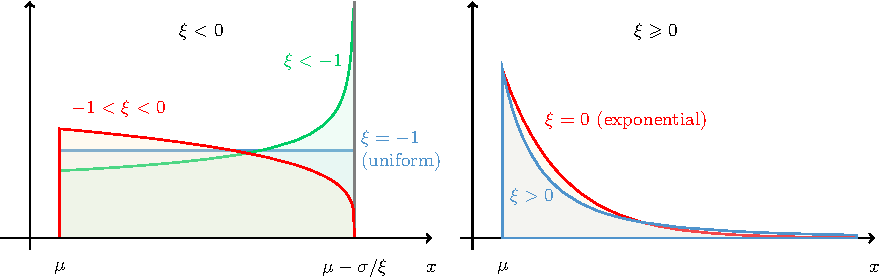
\includegraphics[width=14cm]{images/GPD.pdf}
  \caption{\label{GPDDENS} GPD densities for $\xi <0$ (left) and $\xi \geqslant 0$ (right).
    In the $\xi < 0$ case, the parameters are chosen in order to
    give the same support, i.e. $\mu$ and $-\sigma/\xi$ are kept constant.}
\end{figure}

The value of the shape parameter $\xi$ has a very strong impact, see
figure~\ref{GPDDENS}.

\begin{itemize}
\item When $\xi < 0$ the distribution has a finite upper end-point. 
  As a special case, the uniform 
  \index{uniform distribution}%
  distribution is obtained with $\xi = -1$. The density function
  is decreasing for $ -1 < \xi <0$.
  
\item When $\xi >0$ the density is decreasing.
  The distribution tail thickens as $\xi$ increases.
\end{itemize}
For most practical applications, the range of values for $\xi$ is $(-0.5,\,0.5)$.

     
\subsubsection*{Properties}
%%---------------------
\label{GPDPROP}
The GPD has a finite expectation when $\xi < 1$ and a finite variance 
when $\xi < 1/2$ then given~by
$$ 
    \Esp(X) = \mu + \frac{\sigma}{1-\xi}, \qquad 
    \Var(X) = \frac{\sigma^2}{(1-\xi)^2(1-2\xi)}, \qquad
    \textrm{CV}(Y)= \frac{1}{\sqrt{1-2\xi}}.
$$
The shape parameter $\xi$ can be related to the coefficient of variation.
Note that $\xi>0$ gives $\textrm{CV}(Y)>1$.

For $m>1$ the return level with period~$m$ of~(\ref{eq:MRETURN}) is
$$ 
    x_m = \mu + \sigma \,\left[m^\xi - 1\right]/\xi  
$$
It can be remarked that for any fixed $m$ the value $x_m$ is increasing
with respect to each of the three parameters $\mu$, $\sigma$ and $\xi$
and the same is true for the expectation. Thus increasing any of the three 
parameters leads to a distribution with greater values.

The GPD can be said to be "POT stable" in the following sense. 
If $X \sim\texttt{GPD}(\mu,\,\sigma,\,\xi)$ then for $u \geqslant \mu$
$$
    \Cond{X}{X > u} \sim \texttt{GPD}(u,\,\sigma^\star,\,\xi)
$$
with $\sigma^\star = \sigma + \xi (u-\mu)$. In other words, the upper tail of a GPD density
is a (unnormalized) GPD density see figure~\ref{STABEX}.
\index{POT stability}

\begin{figure}
  \centering
  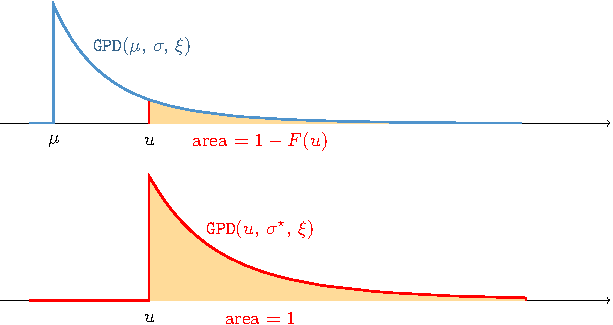
\includegraphics[width=10cm]{images/StableGPD.pdf}
  \caption{\label{STABEX} ``POT stability'' of the GPD family. When 
    $X \sim \texttt{GPD}(\mu,\,\sigma,\,\xi)$ the density of $X$ conditional
    on $X >u$ is $\texttt{GPD}(u,\,\sigma^\star,\,\xi)$ 
    with location $u$ and the shape parameter $\xi$.
  }
\end{figure}


When $\xi < 1$ the GPD corresponds to a linear mean residual life 
\index{mean residual life}%
$$
    \Esp\bCond{X - v}{X > v}  = \frac{ \sigma + \xi \,v }{1 -\xi }
$$ 
This may be used for the determination of the threshold in POT:
replacing the expectation by a sample mean we can check that the 
mean excess life is linear: see \citet[chap.~4]{COLES}.

From the Pickands-Balkema-de Haan theorem, if~$X$ is a random variable
with a distribution in the domain of attraction of the GEV distribution
with shape $\xi$, then distribution of $Y=X-u$ conditional on $X >u$ when $u$
is large will be close to a GPD with shape $\xi$.
%Moreover the psee theorem~4.1 in~\citet{COLES}.  
This property provides a justification for the traditional exclusive
use of the GPD for excesses of POT models. A simple illustration for
the Gumbel case $\xi = 0$ is given page~\pageref{GUMBEXP}.

The GPD has an infinite variance when $\xi \geqslant 1/2$. 
In practice, the values used are generally in the range 
$-0.3 \leqslant \xi \leqslant 0.3$.

\subsubsection*{Estimation and inference}
%%------------------------------------
\index{constraint!inequality in MLE}
In the POT context, the parameter $\mu$ is known since 
it is taken as the threshold~$u$. The excesses
$Y_i:=X_i-u$ are distributed according to the GPD with location 
$\mu=0$ and unknown $\sigma$ and scale $\xi$.

Given an ordinary sample $Y_i$ of size $n$, moments estimators for
$\sigma$ and $\xi$ are readily available
$$
   \widehat{\xi}_{\texttt{mom}} = 
   \frac{1}{2}\,\left[1 - \widehat{\textrm{CV}}^{\,-2}\right], \qquad
   \widehat{\sigma}_{\texttt{mom}} = \frac{\bar{Y}}{2}\,\left[1 + 
     \widehat{\textrm{CV}}^{\,-2}\right].
$$
\index{moment estimation}%
The ML estimation can rely on a two-dimensional maximisation.  Interestingly enough,
the sign of the ML estimator $\widehat{\xi}_{\texttt{ML}}$ has a simple relation with the
empirical coefficient of variation \index{coefficient of variation}
$\widehat{\mathrm{CV}}$. Provided that a 
\label{SignXI}
denominator~$n$ is used to estimate the
variance\footnote{That is $\widehat{\Var}(Y) = \frac{1}{n} \sum_i (Y_i -
  \overline{Y})^2$.}  in~(\ref{eq:CVTHEO}), one can show that $\widehat{\xi} <
0$ is equivalent to $\widehat{\mathrm{CV}} < 1$.  In other words, 
$\widehat{\xi}_{\texttt{mom}}$ and $\widehat{\xi}_{\texttt{ML}}$
have the same sign. This shows that the sign of
the ML estimator $\widehat{\xi}_{\texttt{ML}}$ must be interpreted with care 
since it is not robust to outliers.

It is important to note that when $\xi < 0$ the inequality $-\sigma /
\xi > \max\{ Y_i\}$ must hold, and also that the likelihood tends to
$\infty$ when $- \sigma / \xi \to \max\{ Y_i\}$ with $\xi <
-1$. Therefore, a constraint $\xi \geqslant \xi_{\star}$ with
$\xi_{\star}> -1$ should in theory be imposed in a numerical optimisation,
although the limited precision of computations prevents from converging
to a boundary parameter vector.

%%Note that ML estimators may fail to exist for the GPD in some
%situations.

\subsubsection*{Use in Renext}
%%----------------------------
In \pkg{Renext}, the ML estimation of the two-parameters for an
ordinary sample can be done using the \verb@fGPD@ function.
\index{fGPD estimation function@{\texttt{fGPD} estimation function}}
The estimation is carried out by using either the Lomax or the maxlo
re-parameterisation below (see sections \ref{LOMAX} and \ref{MAXLO}),
depending on the sign of $\widehat{\mathrm{CV}}-1$. In both cases, a
one-dimensional maximisation is used thanks to a concentration of the
likelihood.

The GPD can be used in \verb@Renouv@ under the name \verb@"GPD"@. The 
parameters of (\ref{eq:defGPD}) are named as those of the distribution
names \verb@"gpd"@ the \pkg{evd} package
$$
   \sigma \leftrightarrow \texttt{scale}, \qquad \xi \leftrightarrow \texttt{shape}.
$$
Note that the parameter $\mu$ is used with the name \verb@"loc"@ in the 
distribution functions, but should not be used in the POT context: 
it must then be equal to its default value~$0$, since the distribution is
fitted on the excesses~$Y_i$.

The GPD can also be used under the name \verb@"gpd"@ for compatibility reasons
and is then taken from the \pkg{evd} package. For the ordinary sample (no
historical data) case, \textbf{Renext} then relies on the \verb@evd@
package~\citep{PACKevd} and its \verb@fpot@ estimation function. As
for usual functions related to the distribution (density, distribution, quantile, \dots)
the difference between \verb@"GPD"@ and \verb@"gpd"@ is the the former returns
\verb@NaN@ when an invalid parameter is provided , e.g. a negative value of \verb@scale@,
while the later then produces an error. Sine the \verb@optim@ function can cope with 
a \verb@NaN@ value for the optimised function, \verb@GPD@ is more flexible 
than \verb@gpd@.
\index{GPD vs gpd@{\texttt{GPD} vs \texttt{gpd}}}
\index{GPD (distribution)|)}
\index{evd package@{\textbf{evd} package}}

\subsection{Weibull}
%%------------------
\index{Weibull distribution|(}

\subsubsection*{Definition}
%%-----------------------
The Weibull distribution has a survival function~$S(y)$ and a density function~$f(y)$ given by 
\begin{equation}
  \label{eq:defWeibull}
    S(y) =  e^{-\left(y/\beta\right)^\alpha}, \qquad
  f(y) = \frac{\alpha}{\beta} \left[\frac{y}{\beta}\right]^{\alpha-1} 
  e^{-\left(y/\beta\right)^\alpha}, \qquad
  \qquad y \geqslant 0
\end{equation}
where $\alpha>0$ is the shape parameter and $\beta>0$ the scale 
parameter. 

\subsubsection*{Properties}
%%-----------------------
The Weibull distribution has finite moments at any order with
$$
  \Esp(Y) = \beta \, \Gamma(1 + 1/\alpha), \qquad
  \Var(Y) = \beta^2 \left[\Gamma(1 + 2/\alpha) - \Gamma^2(1 + 1/\alpha)\right], \qquad
  \textrm{CV}(Y) = \sqrt{\frac{\Gamma(1 + 2/\alpha)}{\Gamma^2(1 + 1/\alpha)} - 1}.
$$
The coefficient of variation is strictly decreasing with respect 
to $\alpha$ and takes the value $1$ in the exponential case $\alpha = 1$.
For $\alpha = 0.2$ the CV is about $15.8$ so only values $\alpha > 0.2$
are used in practice.

The properties of the Weibull depend on the shape parameter $\alpha>0$. 

\begin{list}{$\bullet$}{\setlength{\itemsep}{2pt}\setlength{\topsep}{2pt}}
  
\item When $0 < \alpha < 1$, the hazard rate decreases to the
  limit~$0$, and the mean residual life MRL is increasing.
  
\item When $\alpha = 1$ the distribution is exponential with
  constant hazard rate and constant MRL.
  
\item When $\alpha > 1$ the distribution has an increasing hazard rate
  and decreasing MRL.

\end{list}
See~\citet{BAGNOLIBERGSTROM}.

The return level of period $m>1$ is given by $y_m = \beta \,\left[\log
  m\right]^{1/\alpha}$, confirming that the exponential return level
curve $[\log m,\, y_m]$ is convex (concave upwards) for $0 < \alpha <
1$ and (downwards) concave for $\alpha > 1$.

The Weibull distribution is closely related to the exponential.  When
$Y$ is Weibull with shape $\alpha$ the random variable
$Z=Y^{1/\alpha}$ has an exponential distribution.  Thus when $Y$
follows a Weibull distribution $V=-\log Y$ has a Gumbel distribution.

\subsubsection*{Estimation and inference}
%%------------------------------------
The ML estimation is carried out by concentrating the scale parameter
\index{concentration, likelihood}
out of the likelihood. It can be shown that with a suitable re-parameterisation
the concentrated likelihood  is a log-concave function having an unique maximum
easily obtained through a one-parameter maximisation.
Moreover the expected information matrix can be given in closed form. 
These tips are used in \textbf{Renext}.
\index{information matrix!expected}%

The moment estimators are not available in closed form and they can be
obtained only at nearly the same cost as the ML estimators.


\subsubsection*{Goodness-of-fit}
%%----------------------------
Specific tests exist for Weibull distributions but are not implemented
in \textbf{Renext}. The fit can be controlled graphically
with a\textit{ Weibull plot} 
\index{Weibull plot}% 
such as produced by the \verb@weibplot@ function.

\subsubsection*{Use in Renext}
%%----------------------------
The Weibull distribution  can be used in \pkg{Renext} under the name \verb@"weibull"@. The 
parameters of (\ref{eq:defWeibull}) are named as in the \verb@stats@ package from
which the distribution functions are taken
$$
   \beta \leftrightarrow \texttt{scale}, \qquad \alpha \leftrightarrow \texttt{shape}.
$$
The ML estimation with likelihood concentration is available in the 
\verb@fweibull@ function.
\index{fweibull estimation function@{\texttt{fweibull} estimation function}}

This distribution can be used in \verb@Renouv@ as a special 
distribution. It is not necessary to provide initial values for the ML estimation since 
specific initial values are used then in \verb@Renouv@.

\index{Weibull distribution|)}

\subsection{Gamma}
%%-------------------
\index{gamma distribution|(}
\subsubsection{Definition}
%%-----------------------
The gamma distribution  has density
\begin{equation}
  \label{eq:defGamma}
  f(y) = \frac{1}{\Gamma(\alpha) \,\beta^\alpha} \,y^{\alpha-1} e^{-y/\beta} \qquad y \geqslant 0
\end{equation}
where $\Gamma(\alpha)$ denotes the Euler's gamma function,
$\beta>0$ is the scale parameter and $\alpha>0$ is the shape parameter.
The distribution function~$F(y)$ and the survival~$S(y)$ do not have a simple expression.

\subsubsection{Properties}
%%-----------------------
Expectation, variance and coefficient of variation are given by
$$
   \Esp(Y)= \alpha \beta, \qquad \Var(Y) = \alpha \beta^2, \qquad
   \textrm{CV}(Y) = \frac{1}{\sqrt{\alpha}}.
$$
The shape parameter $\alpha$ is related to the coefficient of variation
and $0 < \alpha < 1$ gives $\textrm{CV}(Y)>1$.

\smallskip
The properties of the distribution depend on the shape parameter 
$\alpha>0$.

\begin{list}{$\bullet$}{\setlength{\itemsep}{2pt}\setlength{\topsep}{2pt}}

\item For $0 < \alpha < 1$ the hazard rate decreases to the limit
  $1/\beta$ and the mean residual life MRL increases to the limit~$\beta$

\item For $\alpha=1$ the distribution is the exponential with constant
  hazard and constant MRL,

\item For $\alpha>1$ the hazard rate increases to the limit $1/\beta$
  and the MRL decreases to the limit $\beta$.

\end{list}
See~\cite{BAGNOLIBERGSTROM}.

The gamma distribution is not frequently used to describe extremes,
maybe because it nearly boils down to an exponential with rate $1/\beta$ for
large return periods. In the decreasing hazard case $0 < \alpha < 1$,
it can be considered as a continuous mixture of exponentials with
rates $\lambda > 1/\beta$. 
\index{mixture of exponentials!continuous}

It can be shown that the gamma distribution falls in the domain of
attraction of the Gumbel distribution.  It is a light-tailed
distribution.

\subsubsection{Estimation}
%%-----------------------
Using an ordinary sample~$Y_i$ the moment estimators are readily available
$$
   \widehat{\alpha}_{\texttt{mom}} = \widehat{\textrm{CV}}^{-\,2}, \qquad
   \widehat{\beta}_{\texttt{mom}} = \bar{X}\times \widehat{\textrm{CV}}^{\,2},
$$
\index{moment estimation}%
and these could be used as initial values for a numerical likelihood maximisation. 

As in the Weibull case, it is possible to concentrate
the likelihood and thus to solve a one-parameter maximisation
\index{concentration, likelihood}
problem. Moreover, the maximisation can be reduced to that of a concave 
function, and the \textit{expected} information matrix can be computed. 
\index{information matrix!expected}%

\subsubsection*{Use in Renext}
%%----------------------------
The gamma distribution  can be used in \pkg{Renext} under the name \verb@"gamma"@. The 
parameters of (\ref{eq:defGamma}) are named as in the \verb@stats@ package from
which the distribution functions are taken
$$
   \beta \leftrightarrow \texttt{scale}, \qquad \alpha \leftrightarrow \texttt{shape}.
$$
The ML estimation with likelihood concentration is available in the 
\verb@fgamma@ function.

\index{fgamma estimation function@{\texttt{fgamma} estimation function}}


It is not necessary to provide initial values for the ML estimation since 
specific initial values are used then in \verb@Renouv@.


\index{gamma distribution|)}

\subsection{Log-normal}
%%---------------------
\index{log-normal distribution|(}

\subsubsection{Definition}
%%-----------------------
The log-normal distribution is the distribution of~$e^V$ where $V$ is normal. It
has density
\begin{equation}
  \label{eq:defLogNorm}
  f(y) = \frac{1}{y\,\sigma \sqrt{2\pi}}\, 
  \exp\left\{-\frac{1}{2\sigma^2} \,\left[ \log y - \mu \right]^2 \right\} \qquad y > 0,
\end{equation}
where $\mu$ and $\sigma>0$ are the parameter of the normal distribution of $\log Y$.
The distribution function~$F(y)$ and the 
survival~$S(y)$ do not have simple expression.

Note that these parameters are not the location nor the scale parameter since they
are in the logged scale. 

\subsubsection{Properties}
%%-----------------------
The expectation, variance and coefficient of variation of the log-normal distribution are
$$
  \Esp(Y) = e^{\mu + \sigma^2/2}, \qquad \Var(Y) = \left[e^{\sigma^2} - 1\right] \,e^{2\mu + \sigma^2},
  \qquad \textrm{CV}(Y) = \sqrt{e^{\sigma^2} - 1}.
$$
For the log-normal distribution neither the hazard $h(y)$ nor the mean residual
life $\textrm{MRL}(y)$ are monotonous functions. The mean residual life~$\textrm{MRL}(y)$ is 
reputed\footnote{No proof of this assertion was found.} to be decreasing for large values of~$y$. 

\subsubsection{Estimation and inference}
%%-------------------------------------
The ML estimation from an ordinary sample is straightforward using 
the log transformation which leads to the normal case. 
Exact inference is also available for the parameters. 

However, exact inference for the return levels
or return periods is more complicated. Hence the standard numerical
"delta method" is used in \textbf{Renext}.

\subsubsection{Goodness-of-fit}
%%----------------------------
The fit of the log-normal distribution can be assessed using the 
logged values and a normality test (e.g. Shapiro-Wilk). 
Since the log-normal is not frequently used in POT, such a test is
not in computed in \textbf{Renext}.

\subsubsection*{Use in Renext}
%%----------------------------
The log-normal distribution  can be used in \pkg{Renext} under the name \verb@"lnorm"@. The 
parameters of (\ref{eq:defLogNorm}) are named as in the \verb@stats@ package from
which the distribution functions are taken
$$
   \mu \leftrightarrow \texttt{meanlog}, \qquad \sigma \leftrightarrow \texttt{sdlog}.
$$
It is not necessary to provide initial values for the ML estimation since 
specific initial values are used then in \verb@Renouv@.

\index{log-normal distribution|)}


\subsection{Finite mixture of exponentials}
%%--------------------------------
\index{mixture of exponentials!finite|(}
\subsubsection*{Definition}
%%-----------------------
The finite mixture of exponentials is a distribution with density
(or survival) function obtained as a weighed mean of a finite number
of exponential densities (or survivals) with  different rates. 
For a mixture of two exponentials, the survival function~$S(y)$  
and density~$f(y)$ are given by
\begin{equation}
  \label{eq:defMixExp2}
   S(y) = \alpha_1\,e^{-\lambda_1 y} + (1-\alpha_1)\,e^{-\lambda_2 y}, \qquad
   f(y) = \alpha_1\lambda_1\,e^{-\lambda_1 y} + (1-\alpha_1)\lambda_2\,e^{-\lambda_2 y},
   \qquad y \geqslant 0
\end{equation}
and the parameters are $\alpha_1$, $\lambda_1$ and $\lambda_2$ must verify
\begin{equation}
   \label{eq:MIXEXPCONTR}
   0 < \alpha_1 < 1 \qquad 0 < \lambda_1 < \lambda_2.
\end{equation}
It can be preferable to use the alternative parameter vector
$[\alpha_1,\, \lambda_1, \, \delta]^\top$ with $\delta := \lambda_2-
\lambda_1$, since the constraint $\lambda_1 < \lambda_2$ is replaced
then by the simple constraint~$\delta >0$.


The usual interpretation of a mixture applies: the distribution is
that of a random variable that would be randomly chosen from the
exponential with rate $\lambda_1$ or from the exponential with rate
$\lambda_2$ the respective probabilities being $\alpha_1$ and
$1-\alpha_1$.  In survival analysis the mixture components correspond
to two death rates that may result from two causes of mortality or
from the existence of two sub-populations.


\subsubsection*{Properties}
%%-----------------------
The expectation and uncentered moments have a simple form
$$
   \Esp(Y^\gamma) = \alpha_1/\lambda_1^\gamma + (1-\alpha_1)/\lambda_2^\gamma
$$
for any $\gamma>0$. The coefficient of variation is always greater
than~$1$.

For large values of $y$, the survival~$S(y)$ only depends on the
smallest rate~$\lambda_1$, since
\begin{equation}
    \label{eq:MIXEXPAPP}
    S(y) \underset{y \rightarrow +\infty}{\sim} \alpha_1 \,e^{-\lambda_1 y}.
\end{equation}
The survival analysis context provides a simple interpretation: after
a large time~$y$, the sub-population with smaller death rate
$\lambda_1$ dominates, and the mean residual life therefore increases.

\begin{figure}
  \centering
  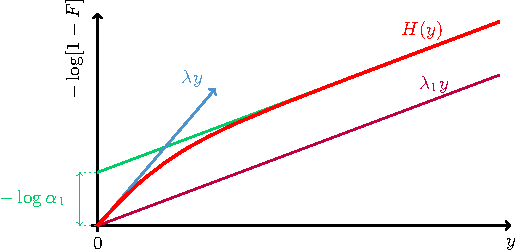
\includegraphics[width=8cm]{images/MixExp2.pdf}
  \caption{\label{MIXEXP} Exponential plot for the distribution
    function of a mixture of two exponentials. The curve shows the
    cumulative hazard $H(y) = -\log[1-F(y)]$.
    The slope of the tangent to the curve
    at the origin is the weighed mean rate~$\lambda = \alpha_1 \lambda_1 + (1-\alpha_1) \lambda_2$. 
    The slope of the asymptote is $\lambda_1$.  Note that $\lambda_1 < \lambda < \lambda_2$.
   }
\end{figure}

It can be shown that the hazard rate function $h(y)$ is decreasing with
a limit $\lambda_1$, and that the mean excess life is increasing with 
a finite limit $1/\lambda_1$. This "rejuvenation effect" results from 
the progressive extinction of the population having the highest death
rate $\lambda_2$. The cumulative hazard $H(y)$ is concave, see 
figure~\ref{MIXEXP}.

The quantile function is not available in closed form and must be
computed numerically.

\subsubsection*{Estimation and inference}
%%------------------------------------
Note that the model would be unidentifiable if the second
constraint of~(\ref{eq:MIXEXPCONTR}) was omitted since the
distribution is invariant under the transformation
$$
   [\alpha_1,\,\lambda_1,\,\lambda_2] \rightarrow [1-\alpha_1,\,\lambda_2,\,\lambda_1].
$$
For an ordinary sample $Y_i$ the ML estimation can be done using
Expectation-Maximisation (EM)
\index{Expectation-Maximisation}%
algorithm.  In this approach, each data $Y_i$ is associated to a
latent variable $Z_i$ with value $z=1$ or $z=2$ indicating the group
(or sub-population) for observation~$i$ and consequently the rate
$\lambda_z$.
%%When the $Z_i$
%are known, ML estimation of parameters is easy (the rates are weighted mean).
%%An iterative procedure computes the expectation of the $Z_i$ and 

In \textbf{Renext} the standard log-likelihood maximisation is used. 
Initial values are computed using the moments when possible, or
using~(\ref{eq:MIXEXPAPP}): regressing
$\log S(y)$ against $y$ for large values of $y$ give 
$-\log \alpha_1$ (intercept) and $\lambda_1$ (slope), see figure~\ref{MIXEXP}. 
Then $\lambda_2$ can be deduced from the sample mean. However
care is needed since these estimates may not fulfil the constraint requirements. 

\subsubsection*{Generalisation}
%%------------------------
A  mixture of $m$ exponentials ($m \geqslant 2$) can be defined through
$$ 
   S(y) = \sum_{i=1}^m \alpha_i\,e^{-\lambda_i y}, \qquad 
   f(y) = \sum_{i=1}^m \alpha_i\lambda_i\,e^{-\lambda_i y}, \qquad 
   y \geqslant 0
$$
with constraints $0 < \alpha_i < 1$, $\sum_i \alpha_i =1$ and 
$0 < \lambda_1 < \lambda_2 < \dots < \lambda_m$
Since the parameter $\alpha_m$ can be dropped as in the $m=2$ case,
the distribution depends on $2m-1$ free parameters.
The behaviour for large~$y$ results from~(\ref{eq:MIXEXPAPP}) which still applies.

The mixture of exponentials is sometimes called \textit{hyper-exponential distribution}.
\index{hyper-exponential distribution}

\subsubsection*{Use in Renext}
%% ---------------------------
The mixture of exponential distributions  can be used in \pkg{Renext} under the name 
\verb@"mixexp2"@, and is currently limited to~$m=2$ exponentials.  
The distribution functions (including the quantile function) are provided
by \pkg{Renext} and use the following names for the  parameters of~(\ref{eq:defMixExp2})
$$
   \alpha_1 \leftrightarrow \texttt{prob1}, \qquad \lambda_1 \leftrightarrow \texttt{rate1},
   \qquad \delta= \lambda_2 - \lambda_1 \leftrightarrow \texttt{delta}.
$$
It is not necessary to provide initial values for the ML estimation since 
specific initial values are used then in \verb@Renouv@.

The ML-based inference for the mixture of exponentials is well known to be 
difficult, and bayesian inference might be a valuable alternative.


\index{mixture of exponentials!finite|)}

\subsection{Lomax}
%%========================
\label{LOMAX}
\index{Lomax distribution|(}%

\subsubsection*{Definition}
%%-----------------------
The \textit{Lomax} distribution depends
on two parameters $\beta>0$ (scale) 
and $\alpha>0$ (shape)  with survival and density functions
\begin{equation}
  \label{eq:SLomax}
  S(y) = \left[1 + \frac{y}{\beta} \right]^{-\alpha}, 
  \qquad
  f(y) = \frac{\alpha}{\beta}\, \left[1 + \frac{y}{\beta} \right]^{-\alpha-1},
  \qquad y > 0.
\end{equation}
This distribution is also known as \textit{Pareto distribution of the second
kind}~\citep{CONTI1}.
\index{Pareto distribution of the second kind}%
When $Y$ is a random variable following this distribution, 
$X= Y +\beta$ is Pareto with minimum~$x_0 =\beta$
and shape~$\alpha$, that is 
$$
   S_X(x) = \left[\frac{x_0}{x} \right]^\alpha, \qquad x > x_0.
$$
\index{Pareto distribution}%
The Pareto distribution with minimum $x_0$ and
shape $\alpha$ is a special case of $\texttt{GPD}(\mu,\,\sigma,\,\xi)$ with 
location $\mu = x_0$, shape $\xi=1/\alpha$ (positive) and the 
extra constraint $\sigma/\xi = x_0$.
The Lomax distribution is the special case of the Generalised Pareto 
$\texttt{GPD}(\mu,\,\sigma,\,\xi)$ with $\mu=0$,
$\sigma = \beta/\alpha$ and $\xi = 1/\alpha$, thus
implying a positive shape parameter~$\xi$.
\index{fixed parameter values}

We can rewrite the distribution function of~$Y$ in the
form~(\ref{eq:BOXCOXED}) below, with $\phi_\alpha(z) \equiv \log z$,
i.e. with the Box-Cox transformation~(\ref{eq:BOXCOXdef}) for $\alpha
=0$. Therefore, the Lomax distribution can be considered as a limit
case of the Shifted Left Truncated Weibull SLTW. We may speak of
\textit{log-exponential distribution} although the expression is
ambiguous.  

\index{log-exponential distribution}%

\subsubsection*{Properties}
%%-----------------------
The quantile function is available in closed form.
The expectation is finite only for $\alpha > 1$ and the variance is finite 
only for $\alpha>2$.
In this case
$$
   \Esp(Y) = \frac{\beta}{\alpha-1},   \qquad 
   \Var(Y) = \frac{\alpha \,\beta^2}{(\alpha-1)^2(\alpha-2)}, \qquad
   \textrm{CV}(Y) = \sqrt{\frac{\alpha}{\alpha-2}} >1.
$$
Only the cases with $\alpha>2$ seem practicable. Then $\textrm{CV}(Y)$
will be close to~$1$ for a large shape~$\alpha$.

The Lomax distribution has a decreasing hazard rate and a linearly
increasing Mean Residual Life.

If both $\alpha$ and $\beta$ tend to $\infty$ with $\alpha/\beta$
tending to $\lambda >0$ then the Lomax distribution tends to the
exponential with rate $\lambda$.

It can be shown that this distribution
is a (continuous) gamma mixture of exponentials.  
\index{mixture of exponentials!continuous} 
More precisely, the survival of~(\ref{eq:SLomax}) can
be written as
$$ 
S(y) = \int_{0}^{+\infty} g(\lambda) \, e^{-\lambda y}
\,\mathrm{d}\lambda
$$
\index{gamma distribution}%
where $g(\lambda)$ is the density of the gamma distribution with shape
$\alpha_{\texttt{gam}}:=\alpha$ and scale $\beta_{\texttt{gam}} := 1/\beta$. The
survival $S(y)$ is thus the weighed mean of the exponential survivals
$e^{-\lambda y}$ with the weight function $g(\lambda)$. Contrary to 
the finite mixture of exponentials which behaves for large return periods 
as does its component with the smallest rate~(\ref{eq:MIXEXPAPP}), 
this continuous mixture is heavy tailed. The reason is that
$g(\lambda)$ weights small rates $\lambda \approx 0$, and thus the mixture 
embeds exponentials with arbitrarily large means~$1/\lambda$. The survival function is a 
\textit{completely monotone} function \citep{FELLER2}.
\index{completely monotone function}

\subsubsection*{Estimation}
%%-----------------------
When the two parameters $\beta>0$ and $\alpha>0$ are unknown, the ML
estimators from an ordinary sample $Y_i$ can be found using a
one-dimensional optimisation by concentrating the shape parameter~$\alpha$ out
\index{concentration, likelihood}
of the likelihood. Although the concentrated log-likelihood
$\ell_{\texttt{c}}(\beta)$ is not concave, it can be proved to have a
maximum\footnote{Our proof states that a global maximum exists, but
  not that it is unique.} when 
the sample $\textrm{CV}$ is
greater than~$1$.  Moreover the expected information matrix is
available in closed form~\citep{LomaxBias}.  The ML estimates fail to exist when the
sample coefficient of variation $\textrm{CV}$ is less than~$1$. The
estimation may also fail when $\textrm{CV}$ is greater than, yet close
to~$1$.
\index{information matrix!expected}%

When $\beta$ is known, the estimation boils down to that of the 
exponential distribution since $V:= \log[1 + Y/\beta]$ then follows
an exponential distribution with rate~$\alpha$.

%%Exact inference is available, 
%%but is not implemented as such in \textbf{Renext} with the \verb@spareto@
%%distribution. 

\subsubsection*{Use in Renext}
%%---------------------------
This distribution is provided in \pkg{Renext} under the name \verb@"lomax"@. The
names of the formal arguments for the parameters in the probability functions are
\begin{center}
  $\beta \leftrightarrow$ \verb@scale@, \qquad
  $\alpha \leftrightarrow$ \verb@shape@. 
\end{center}
The ML estimation with likelihood concentration 
is available in the \verb@flomax@ function. This function rescales the 
data to avoid numerical problems.
\index{rescaling (data)}
\index{flomax estimation function@{\texttt{flomax} estimation function}}

This distribution is recognized as special in \verb@Renouv@, thus providing a simple
mean to impose the constraint $\xi>0$ for excesses assumed to
follow $\texttt{GPD}(0,\,\sigma,\,\xi)$. 

Estimation and exact inference are possible in the case where the
shift $\beta$ is taken as the (known) threshold i.e. $\beta =
u$. The exponential distribution should then be used with a
logarithmic transformation as explained below in~\ref{TRANSEXP}. The
two formal arguments and values to use in the \verb@Renouv@ call
are \verb@distname.y = "exponential"@ and \verb@trans.y = "log"@. Note that
$\alpha$ is then obtained with the name \verb@"rate"@, and its estimated value
will be greater than~$1$.
\index{Lomax distribution|)}


\subsection{Maxlo}
%%========================
\label{MAXLO}
\index{maxlo distribution|(}%
\subsubsection*{Definition}
%%-----------------------
Though very useful in POT models, this distribution does not seem  
to have deserved its own name yet. We decided to call it "maxlo" as a pun 
inspired by a kind of symmetry to the Lomax distribution.

The \textit{maxlo} distribution depends on two parameters $\beta>0$ (scale) 
and $\alpha>0$ (shape). The support of the distributions is $[0,\,\beta]$ 
and the survival and density functions are
\begin{equation}
  \label{eq:Smaxlo}
  S(y) = \left[1 - \frac{y}{\beta} \right]^{\alpha}, 
  \qquad f(y) = \frac{\alpha}{\beta}\,\left[1 - \frac{y}{\beta} \right]^{\alpha-1} \qquad 0 < y < \beta.
\end{equation}
The maxlo  distribution is the special case of the Generalised Pareto 
$\texttt{GPD}(\mu,\,\sigma,\,\xi)$ with $\mu=0$,
$\sigma = \beta/\alpha$ and $\xi = -1/\alpha$, thus
implying a \textit{negative shape}~$\xi$.
\index{fixed parameter values}

\subsubsection*{Properties}
%%-----------------------
The quantile function is available in closed form.  
This distribution has finite moments of any order and
$$
\Esp(Y) = \frac{\beta}{\alpha+1},   \qquad 
\Var(Y) = \frac{\alpha \,\beta^2}{(\alpha+1)^2(\alpha+2)}, \qquad
\textrm{CV}(Y) = \sqrt{\frac{\alpha}{\alpha + 2}} < 1.
$$
Note that $\textrm{CV}(Y)$ will be close to $1$ for large values of
the shape~$\alpha$.

If both $\alpha$ and $\beta$ tend to $\infty$ with $\alpha/\beta$ tending to 
$\lambda >0$ then the maxlo distribution tends to the exponential with rate $\lambda$.

\subsubsection*{Estimation}
%%-----------------------
\index{constraint!inequality in MLE}
When the two parameters $\beta>0$ and $\alpha>0$ are unknown, the ML estimators
from an ordinary sample $Y_i$ can be found using a one-dimensional optimisation
by concentrating the shape parameter~$\alpha$ out of the likelihood. Note
that the inequality constraint $\beta>\max \{Y_i\}$ must hold and that the 
likelihood tends to $\infty$ when $\beta \to \max \{Y_i\}$ with $\alpha < 1$.
So in practice an inequality $\alpha \geqslant \alpha_{\texttt{L}}$ must
be imposed for some $\alpha_{\texttt{L}} > 1$.

Although \index{concentration, likelihood} the concentrated
log-likelihood $\ell_{\texttt{c}}(\beta)$ is not concave it can be
proved to have a maximum\footnote{Our proof states the existence of
  local maximum.} when the sample $\textrm{CV}$ is smaller than~$1$,
thus mirroring the property stated for the Lomax distribution.
Moreover the expected information matrix is available in closed form.
The ML estimates fail to exist when the sample coefficient of
variation $\textrm{CV}$ is greater than~$1$. The estimation may also
fail when $\textrm{CV}$ is smaller than yet close to~$1$.
\index{information matrix!expected}%



When $\beta$ is known, the estimation boils down to that of the 
exponential distribution since $V:= -\log[1 - Y/\beta]$ follows
an exponential distribution with rate~$\alpha$.


%%Exact inference is available, 
%%but is not implemented as such in \textbf{Renext} with the \verb@spareto@
%%distribution. 

\subsubsection*{Use in Renext}
%%---------------------------
This distribution is provided in \pkg{Renext} under the name \verb@"maxlo"@. The
names of the formal arguments for the parameters in the probability functions are
\begin{center}
  $\beta \leftrightarrow$ \verb@scale@, \qquad
  $\alpha \leftrightarrow$ \verb@shape@. 
\end{center}
The ML estimation with likelihood concentration 
is available in the \verb@fmaxlo@ function.
\index{fmaxlo estimation function@{\texttt{fmaxlo} estimation function}}
This function rescales the 
data to avoid numerical problems.
\index{rescaling (data)}

This distribution can be used in \verb@Renouv@, thus providing a simple
mean to impose the constraint $\xi<0$ for excesses assumed to
follow $\texttt{GPD}(0,\,\sigma,\,\xi)$. 

\index{maxlo distribution|)}



\subsection{Transformed Exponential distributions}
%%============================================
\label{TRANSEXP}
\index{transformed exponential|(}
\subsubsection*{Definition}
%%----------------------
This rather informal family of distributions is sometimes used in hydrology.
Although we will only consider in practice the two functions 
$\phi(x) = x^2$ and $\phi(x) = \log x$ both for $x>0$,
a slightly more general framework can be proposed as follows. 
Let $\phi(x)$ be a regular and strictly increasing function
defined for $x > x_0$ and let $u$ be a known value $u > x_0$. When a random
variable
$X$ is such that
$$ 
   \phi(X) - \phi(u) \sim \texttt{Exp}
$$
we may say that $X$ has a \textit{transformed exponential} distribution. 
The values of this distribution are the real numbers~$x$ with $x>u$.
Note that the transformation needs to be one-to-one, because the distribution 
of $X$ must be determinable from that of $Z=\phi(X) - \phi(u)$. Then
$$ 
    X = \psi\left(Z + \phi(u)\right)
$$
where $\psi(z)$ is the reciprocal function of $\phi(x)$.
As an example, the square transformation can be applied only for~$x>0$.

The survival function is given by 
$$ 
   S_X(x) =  \exp\left\{-\nu \left[ \phi(x) - \phi(u) \right]\rule{0pt}{0.9em}\right\}
   \qquad x > u
$$
where $\nu>0$ is the rate of the exponential distribution. The density comes 
by derivation.

\subsubsection*{Properties}
%%-----------------------
The properties of the distribution obviously depend on the choice of the 
transformation. 
\begin{list}{$\bullet$}{ }
  \item For the square transformation $\phi(x) = x^2$ we get a 
    shifted and truncated Weibull distribution as described below. It
    may be called \textit{square-exponential} or (in french) \textit{loi en carr\'e}. 
    \index{square-exponential distribution} 
    \index{loi en carres@{\textit{loi en carr\'e}}}
  \item With  the logarithmic  transformation $\phi(x) = \log x$ we get a shifted version 
    of the Pareto (heavy tailed) distribution called Lomax distribution 
    and  described above in~\ref{LOMAX}. It
    may  be called \textit{log-exponential}. 
    \index{log-exponential distribution} 
  \end{list}
The quantile function is available in closed form provided that the
reciprocal function $\psi(z)$ is such.  This is actually the 
case for the two transformations considered.


\subsubsection*{Estimation and inference}
%%-------------------------------------
As far as an ordinary sample $X_i$ is used, the ML  estimator~$\widehat{\nu}$ of 
the rate~$\nu$ is available  using the mean  of the transformed 
random variables~$Z_i = \phi(X_i)-\phi(u)$
$$ 
    1/\widehat{\nu} = \bar{Z} = \overline{\phi(X})-\phi(u)
$$ 
Exact inference on $\nu$ is deduced from the exponential case.

\subsubsection*{Use in Renext}
%%---------------------------
The package allows the use of two transformed exponential 
distributions with the \verb@Renouv@ function, 
where $u$ \textit{is necessarily taken as equal to
the threshold}. The value given for the  transformation formal 
argument \verb@trans.y@  can be 
either \verb@"square"@ or \verb@"log"@. 
In both cases, the exponential distribution must be specified by giving
the value \verb@"exponential"@ to the distribution argument 
\verb@distname.y@.

\index{transformed exponential}

\subsection{Shifted Left Truncated  Weibull (SLTW) distribution}
%%============================================
\label{SLTW}
\subsubsection*{Definition}
%%--------------------- 
We call (shifted) \textit{left truncated Weibull} (SLTW) the following 
distribution for a random variable~$Y > 0$. 
\index{SLTW distribution}
\index{shifted left truncated Weibull|see{SLTW}}
It depends  on three parameters  $\delta>0$ (shift or location), $\beta>0$ (scale) 
and $\alpha >0$ (shape) and has survival function 
\begin{equation}
  \label{eq:SLTWF}
  S(y) =  
  \exp\left\{- \left[ \left(\frac{y+\delta}{\beta} \right)^\alpha 
      -\left(\frac{\delta}{\beta}\right)^\alpha \right] \right\} 
  \qquad y > 0 
\end{equation}
The density comes by derivation.  This is the conditional distribution 
$\Cond{X-\delta}{X>\delta}$ where $X$ has Weibull distribution with shape $\alpha$ and scale 
$\beta$. \index{Weibull distribution}

For $\alpha=2$ we can rewrite the survival as
$$
   S(y) = \exp\left\{-\nu \left[(y+\delta)^2 - {\delta}^2 \right]\right\} 
   \qquad y > 0
$$
thus the distribution is identical to the square-exponential described previously.
\index{square-exponential distribution}
\index{loi en carres@{\textit{loi en carr\'e}}}

\begin{figure}
  \centering
  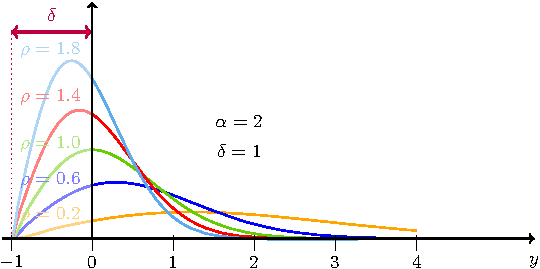
\includegraphics[width=10cm]{images/SqExp.pdf}
  \caption{\label{SQEXP}
    "Square exponential" densities, i.e. SLTW densities with shape 
    $\alpha=2$. 
    Only the part $y \geqslant 0$ of the Weibull densities is used and the normalisation
  is on the interval $y \geqslant 0$.}
\end{figure}


This three parameter family can be used for excesses in POT, but 
in a general framework there is no natural choice for $\delta>0$ in relation
with a physical threshold~$u$, though the two quantities have the
same physical dimension. For some applications of POT where the random 
variable is 
positive $\delta$ is sometimes chosen as the threshold $\delta = u$.

\subsubsection*{Properties}
%%-----------------------
%% The three parameter family is (by construction) POT stable for positive thresholds. 
The moments or even the expectation are not easily computed in the general 
case.  
%% \index{POT stability}

For $\alpha \leqslant 1$ the mode of $Y$ is always $y=0$. For $\alpha>1$  the mode of
$Y$ is the positive part $y_+^\star$ of the shifted mode $y^\star$ of the Weibull i.e.
$y^\star = \left(\alpha - 1\right)^{1/\alpha}\beta - \delta$. 
Thus for a fixed $\alpha$ and $\delta$ we can
have a mode varying with~$\beta$.

The quantile function is available in closed form. 
The hazard and the MRL for this distribution are merely truncations
of their equivalent for the Weibull distribution, e.g. the hazard is 
decreasing for $0 \leqslant \alpha <1$ and 
increasing for $\alpha>1$.

For $\alpha>0$ and large~$\delta$, the 
distribution is close to the exponential since the Weibull distribution
is in the domain of attraction of the Gumbel distribution for which the 
excesses over a large threshold tend to be exponentially distributed.

Using the notation $\rho = \alpha/\beta^\alpha$ we can
rewrite the survival as
\begin{equation}
    \label{eq:BOXCOXED}
    S(y) = 
    \exp \left\{ - \rho\, \left[ 
        \phi_\alpha(y + \delta)
          -\phi_\alpha (\delta)  
        \right] \right\} \qquad y > 0, 
\end{equation}
where $\phi_\alpha(z)$ is the Box-Cox transformation defined for $z>0$ by
\begin{equation}
  \label{eq:BOXCOXdef}
   \phi_\alpha(z) = 
   \begin{cases} 
     (z^\alpha - 1)/\alpha & \alpha > 0\\
     \log z                & \alpha = 0. 
   \end{cases}
\end{equation}
The function $\phi_\alpha(z)$ is strictly increasing with limit $+\infty$ when 
$z \rightarrow +\infty$ and it is regular with respect 
to~$\alpha$ for $\alpha=0$.
Thus if $\alpha$ and $\beta$ both
tend to zero in such way that $\rho$ tends to a limit $\rho^\star>0$ the
distribution tends to the Lomax distribution described above. The
limit survival is~(\ref{eq:BOXCOXED}) with $\alpha=0$ and 
$\rho=\rho^\star$.


\subsubsection*{Estimation}
%%------------------------
In most contexts, the shift parameter $\delta$ should be known and given. 

Note that when  both $\alpha$ and $\delta$ are known and
when the estimation is from an ordinary sample $Y_i$ of size~$n$,
the ML estimator~$\widehat{\rho} = \alpha/\beta^\alpha$ of~$\rho$ is available 
using the mean of the transformed $Y_i$
$$ 
    1/\widehat{\rho} = \overline{\phi_\alpha(Y+\delta)}-\phi_\alpha(\delta)
$$ 
Exact inference on $\rho$ or on the quantiles is then easily deduced from the exponential case.
\index{exact inference}

\subsubsection*{Use in Renext}
%%---------------------------
The SLTW distribution is provided in \pkg{Renext} under the name \verb@SLTW@.
The relevant probability functions share the three following formal 
arguments for the parameters, in correspondence with~(\ref{eq:SLTWF})
\begin{center}
  $\delta \leftrightarrow$ \verb@delta@, \qquad
  $\alpha \leftrightarrow$ \verb@shape@, \qquad
  $\beta \leftrightarrow$ \verb@scale@. 
\end{center}
Note that the parameter named \verb@scale@ \textit{is not} a scale parameter in the 
usual statistical sense; the name only refers to the original Weibull distribution.

No specific inference method is implemented in the \pkg{Renext} POT
fitting. A special case is when $\delta$ is equal to the (known) threshold~$u$
and when moreover $\alpha$ is known. Indeed, we then fit an exponential distribution 
to a transformed  version $\phi_\alpha(X)$ of the level $X \equiv Y +u$.
We thus can use in the special case where $\alpha=2$ (square transformation)
and the limit case where $\alpha = 0$ (log transformation) as explained
above in~\ref{TRANSEXP}.
In the \verb@Renouv@ function, one must then use
\verb@distname.y = "exponential"@; the transformation argument 
must be respectively \verb@trans.y = "square"@ and \verb@trans.y = "log"@. 


\subsection{Other distributions}
%%---------------------------
It is possible to use a quite arbitrary distribution within the \verb@Renouv@
function provided the probability functions\footnote{Density, distribution and quantile
functions are required.}
are available in~R and satisfy the conditions stated in the help of the \verb@Renouv@ 
function.



%%\nocite*
%% \bibliography{Renext}
%%\bibliographystyle{jss}

\bibliography{Renext}

\printindex
\end{document}
